%% ESTRUTURA DO DOCUMENTO
\documentclass[PublicacaoDissOuTese,brazilian]{tdiinpe}

%% TEXTO EM ARIAL
%\renewcommand{\rmdefault}{phv} % Arial
%\renewcommand{\sfdefault}{phv} % Arial

%% PUBLICAÇÃO EM INGLÊS
% renomear o arquivo: abnt-alf.bst para abnt-alfportuguese.bst
% renomear o arquivo: abnt-alfenglish.bst para abnt-alf.bst

\usepackage{verbatim}
\usepackage[utf8x]{inputenc}
\usepackage{rotating}
\usepackage{dsfont}
\usepackage[all]{xy}
\usepackage[all]{pstricks}
\usepackage{enumerate}
%\watermark{Revisão No. 50}
%% CAPA DO DOCUMENTO
\serieinpe{INPE-NNNNN-TDI/NNNN}

\titulo{IMPACTO DA ASSIMILA\c{C}\~{A}O DE DADOS DE PRECIPITA\c{C}\~{A}O NO SISTEMA RPSAS/CPTEC: UM ESTUDO DE CASO DE COMPLEXO CONVECTIVO DE MESOESCALA}
\title{IMPACT OF PRECIPITATION ASSIMILATION IN CPTEC'S RPSAS SYSTEM: A CASE STUDY OF MESOSCALE CONVECTIVE SYSTEM} 
\author{Carlos Frederico Bastarz}
\descriccao{Dissertação de Mestrado do Curso de Pós-Graduação em Meteorologia, orientada pelos Drs. Dirceu Luis Herdies e Julio Pablo Reyes Fernandez, Março de 2010.}
\repositorio{xxx}

\date{2010}

%% VERSO DA CAPA
\tituloverso{\vspace{-0.9cm}\textbf{\PublicadoPor:}}
\descriccaoverso{Instituto Nacional de Pesquisas Espaciais - INPE\\
Gabinete do Diretor (GB)\\
Serviço de Informação e Documentação (SID)\\
Caixa Postal 515 - CEP 12.245-970\\
São José dos Campos - SP - Brasil\\
Tel.:(012) 3945-6911/6923\\
Fax: (012) 3945-6919\\
E-mail: {\url{pubtc@sid.inpe.br}}
}

%% FOLHA DE ROSTO
\descriccaoversoA{\textbf{\ConselhoDeEditoracao:}\\
\textbf{\Presidente:}\\
Dr. Gerald Jean Francis Banon - Coordenação Observação da Terra (OBT)\\
\textbf{\Membros:}\\
Drª Maria do Carmo de Andrade Nono - Conselho de Pós-Graduação \\
Dr. Haroldo Fraga de Campos Velho - Centro de Tecnologias Especiais (CTE)\\
Drª Inez Staciarini Batista - Coordenação Ciências Espaciais e Atmosféricas (CEA)\\
Marciana Leite Ribeiro - Serviço de Informação e Documentação (SID)\\
Dr. Ralf Gielow - Centro de Previsão de Tempo  e Estudos Climáticos (CPT)\\
Dr. Wilson Yamaguti - Coordenação Engenharia e Tecnologia Espacial (ETE)\\
\textbf{\BibliotecaDigital:}\\
Dr. Gerald Jean Francis Banon - Coordenação de Observação da Terra (OBT)\\
Marciana Leite Ribeiro - Serviço de Informação e Documentação (SID)\\
Jefferson Andrade Ancelmo - Serviço de Informação e Documentação (SID)\\
Simone A. Del-Ducca Barbedo - Serviço de Informação e Documentação (SID)\\
\textbf{\RevisaoNormalizacaoDocumentaria:}\\
Marciana Leite Ribeiro - Serviço de Informação e Documentação (SID) \\
Marilúcia Santos Melo Cid - Serviço de Informação e Documentação (SID)\\
Yolanda Ribeiro da Silva Souza - Serviço de Informação e Documentação (SID)\\
\textbf{\EditoracaoEletronica:}\\
Viveca Sant'Ana Lemos - Serviço de Informação e Documentação (SID)\\
}

%% FICHA CATALOGRAFICA
\cutterFICHAC{Cutter}
\autorUltimoNomeFICHAC{Bastarz, Carlos Frederico}
\autorAbreviadoFICHAC {}
\tituloFICHAC{IMPACTO DA ASSIMILAÇÃO DE DADOS DE PRECIPITAÇÃO NO SISTEMA RPSAS/CPTEC: UM ESTUDO DE CASO DE COMPLEXO CONVECTIVO DE MESOESCALA}
\instituicaosigla{INPE}
\instituicaocidade{São José dos Campos}
\paginasFICHAC{\pageref{numeroDePáginasDoPretexto} + \pageref{LastPage}}
\serieinpe{INPE-00000-TDI/0000}
\palavraschaveFICHAC{1.~Assimilação de Dados. 2.~Precipitação. 3.~Nudging. 4.~TRMM. 5.~Complexo Convectivo de Mesoescala.  I.~\mbox{Título}.}
\numeroCDUFICHAC{000.000} 

%% NOTA DA FICHA (PARA TD)
\tipoTD{Dissertação}
\cursoFA{Mestrado em Meteorologia}
\instituicaoDefesa{Instituto Nacional de Pesquisas Espaciais}
\anoDefesa{2010} 
\nomeAtributoOrientadorFICHAC{Orientadores}
\valorAtributoOrientadorFICHAC{Dirceu Luis Herdies e Julio Pablo Reyes Fernandez} % nome(s) completo(s)

%% FOLHA DE APROVACAO PELA BANCA EXAMINADORA
\tituloFA{\textbf{ATENÇÃO! A FOLHA DE APROVAÇÃO SERÁ INCLUIDA POSTERIORMENTE.}}
%\cursoFA{\textbf{}}
\candidatoOUcandidataFA{Carlos Frederico Bastarz}
\dataAprovacaoFA{26 de Março de 2010}
\membroA{Dr. José Paulo Bonatti}{}{}
\membroB{Dr. Adilson Wagner Gandú}{}{}
\membroC{Dr. Carlos Frederico de Angelis}{}{}
\membroD{Dr. Julio Pablo Reyes Fernandez}{}{}
\membroE{Dr. Dirceu Luis Herdies}{}{}
\membroF{}{}{}
\membroG{}{}{}
\ifpdf

%% NIVEL DE COMPRESSAO {0 -- 9}
\pdfcompresslevel 9
\fi

%% DEFINE EM 80% A LARGURA DAS FIGURAS
\newlength{\mylenfig} 
\setlength{\mylenfig}{0.8\textwidth}

%% COMANDOS PESSOAIS
\newcommand{\vetor}[1]{\mathit{\mathbf{#1}}}

\makeindex

\begin{document}
%% CAPAS E OUTRAS ESTRUTURAS
\maketitle
%% EPIGRAFE
\begin{epigrafe}
\hypertarget{estilo:epigrafe}{}
\textit{\large``Na vida nunca se deveria cometer duas vezes o mesmo erro: há bastante por onde escolher".}
\vspace{1cm}
\hspace{4cm} \emph{\textsc{Bertrand Russell}}
\end{epigrafe}

%% DEDICATORIA
\begin{dedicatoria}
\hypertarget{estilo:dedicatoria}{}
\newcommand{\mytext}{À memória de meus pais.}
\ifcalligra
	\calligra\Large \mytext
\else
	\itshape\Large \mytext 
\fi
\end{dedicatoria}

%% AGRADECIMENTOS
\begin{agradecimentos}
\hypertarget{estilo:agradecimentos}{}

Em primeiro lugar, agradeço a Deus pela vida. Aos sentimentos que me permitem amar e fazer feliz. Às pessoas que assim o fazem sem a pretensão de seguir-me.

A meus pais, Friedrich e Mirian, que me criaram e me proveram com seu amor, carinho. À minha irmã Beatriz pela sua cumplicidade, respeito e amor.

À Helena, pelo seu amor, paciência, cumplicidade e inefável companheirismo.

Aos amigos Weber, Rogério, Isabel Pilotto, Diego, Marília, Ricardo, Paulo, Dayana, Jairo, Francisco e Tania. Agradeço, em primeiro lugar, pela amizade conquistada. Agradeço também, imensamente, à ajuda que me prestaram nos momentos em que mais precisei. Obrigado pelo companheirismo.

À Rita e Tatiane, pela ajuda nos trabalhos e pelos exemplos de vida.

Aos meus professores de graduação Aury, Maria de Fátima, Vera Lia, Angela, Geraldo e Tania. Agradeço pela confiança e orientação, pelas recomendações e oportunidades que me deram.

Aos meus orientadores de mestrado Dirceu e Pablo, pela orientação e ajuda. Obrigado pela cumplicidade, pela confiança que creditaram em mim e pelos ensinamentos.

Ao João, pela amizade, pela ajuda prestada com os diversos programas, scripts, modelos, ideias e conceitos. Ao Sapucci pelo grande auxílio na manutenção do RPSAS, gerenciamentos dos scripts, ideias e observações.

Ao grupo de Assimilação de Dados do CPTEC/INPE, pelo apoio durante as reuniões do GEDAI, pela iniciativa e comprometimento.

Ao Marcos Mendonça e à Renata pela ajuda com o programa para acumular a precipitação do TRMM.

Ao Rildo pelo seu auxílio com os scripts e explicações sobre a avaliação dos modelos de previsão.

Às secretárias do Curso de Pós-Graduação em Meteorologia do INPE, Lilian, Fabiana e Simone. Ao Gilson, Marcela e Michele, secretários da DMD. Obrigado pelos auxílios que prestaram nos momentos burocráticos, pela atenção e simpatia.

À PGMET pela ajuda concedida a mim em momentos difíceis durante a minha caminhada.

A todos os colegas que, embora não citados aqui, colaboraram para o desenvolvimento deste trabalho, seja com sugestões e apontamentos ou simplesmente pela compreensão de quem sou.

Ao CPTEC/INPE pelo uso de suas instalações para o desenvolvimento deste trabalho.

À Comunidade do Software Livre e às pessoas que dispõem de seu tempo livre para construir os programas e scripts, sem os quais, boa parte da pesquisa realizada em diversas áreas seria mais complicada e demorada. 

À FAPESP (Fundação de Amparo à Pesquisa do Estado de São Paulo) pela concessão da bolsa de mestrado e financiamento do projeto No. 2007/06256-6.

\end{agradecimentos}

%% RESUMO
\begin{resumo}
\hypertarget{estilo:abstract}{}

O presente trabalho apresenta os resultados de um estudo de impacto da assimilação de dados de precipitação estimada do \textit{Tropical Rainfall Measuring Mission} (TRMM) no \textit{Regional Physical-space Statistical Analysis System} (RPSAS) do Centro de Previsão de Tempo e Estudos Climáticos (CPTEC), durante  o mês de janeiro de 2003. Neste estudo, a assimilação de dados de precipitação foi realizada durante a geração do \textit{first guess} pelo modelo regional Eta de 20 $km$ do CPTEC utilizando-se a técnica de \textit{nudging}. A partir deste \textit{first guess}, o sistema de assimilação de dados RPSAS gera uma análise sobre um domínio que cobre grande parte da América do Sul, a partir da qual foram produzidas previsões de 24 horas utilizando o modelo Eta. Dados da reanálise global 2 do NCEP/DOE e regional do CPTEC foram utilizados para comparação com as análises geradas com e sem a assimilação de dados de precipitação. Dados coletados durante a campanha do \textit{South American Low-Level Jet EXperiment} (SALLJEX), do \textit{Global Precipitation Climatology Project} (GPCP) e TRMM foram utilizados para comparação com as previsões do modelo Eta. A avaliação dos resultados foi feita com base em índices estatísticos e mostrou que o desempenho das previsões de até 24 horas do modelo Eta, principalmente nas primeiras horas, é sensivelmente melhor com a inclusão da precipitação, apresentando valores de Viés e Erro Quadrático Médio menores, se comparado com o mesmo modelo sem a assimilação de precipitação. Foi realizado também um estudo de caso de Complexo Convectivo de Mesoescala (CCM) ocorrido durante a campanha do (SALLJEX). A inclusão da assimilação de precipitação no ciclo do sistema Eta+RPSAS permitiu simular um caso de CCM ocorrido em 23 de Janeiro de 2003 com maiores detalhes, onde foi comparada a precipitação produzida pelo modelo Eta com a precipitação observada durante o SALLJEX e também com o GPCP e TRMM. Foram comparados também os perfis de vento das análises do RPSAS com a reanálise do NCEP durante a ocorrência do CCM e encontrou-se maior concordância entre os perfis, em relação aos perfis produzidos sem a assimilação de precipitação. Os fluxos meridionais de umidade calculados também mostraram valores semelhantes aos valores produzidos pela reanálise do NCEP. Os resultados destas simulações mostram também que além do modelo Eta, com assimilação de precipitação, ser capaz de reproduzir com maior detalhamento algumas das principais características do CCM, como a distribuição espacial de precipitação observada, os níveis pluviométricos produzidos pelo modelo de previsão foram melhorados. Neste estudo foi possível também verificar que o uso da assimilação de precipitação do TRMM na geração do \textit{first guess} melhorou a análise regional produzida pelo sistema de assimilação RPSAS do CPTEC e, consequentemente, incrementou a previsão de 24 horas produzida pelo modelo Eta do centro. A partir dos resultados obtidos e, realizando-se alguns ajustes ao esquema de assimilação propostos, pode-se estudar a possibilidade de se implementar operacionalmente a assimilação de precipitação do TRMM no sistema de assimilação/previsão regional Eta+RPSAS do CPTEC com o objetivo de contribuir para o aumento da qualidade das previsões regionais do centro, principalmente as de curto prazo além de incrementar esse sistema com o aproveitamento de mais uma fonte de dados de observações de precipitação.

\end{resumo}

%% ABSTRACT
\begin{abstract}
\hypertarget{estilo:abstract}{}

This work presents the results of a impact study of estimated precipitation data assimilation in RPSAS from CPTEC, during January 2003. In this study, the precipitation assimilation was performed during the generation of first guess by the regional Eta model using a methodology similar to nudging. From this first guess, the RPSAS system generates an analysis with 20 $km$ horizontal resolution in an area that covers South America, from which were produced 24 hours forecasts using the Eta model. Global reanalysis data from NCEP/DOE and regional reanalysis data from CPTEC were used for comparison with the tests generated with and without the precipitation assimilation. Data collected during the SALLJEX campaign, TRMM and GPCP were used for comparison with the predictions of the Eta model. The evaluation of the results was made based on statistical indices and showed that the performance of forecasts up to 24 hours of the Eta model, especially in the early hours, is significantly enhanced by the inclusion of precipitation. The values of Bias and Mean-Square Error compared with the same model without the assimilation of precipitation were minor. Also was carried out a case study of Mesoscale Convective Complex occurred during the SALLJEX campaign. The inclusion of the precipitation assimilation in the Eta+RPSAS forecasts/analysis cycle allowed to simulate a case of MCC occurred on 23 January 2003 with more details. Was also compared the wind profiles from the RPSAS analysis with the NCEP reanalysis for the occurrence of the MCC and were found a greater concordance between the profiles in relation to the profiles produced without the precipitation assimilation. Moisture flux was also calculated and showed similar values to the values produced by the NCEP reanalysis. The results of these simulations also show that besides the Eta model with precipitation assimilation, is able to play in more detail some key features of the MCC, as the spatial distribution of observed precipitation. Also the rainfall levels produced by the forecast model have been improved. This experiment also found that the use of the assimilation of TRMM precipitation in the generation of first guess improved the regional analysis produced by the CPTEC's RPSAS assimilation system and therefore increased the 24 hours forecasts produced by the Eta model. From the results, and making a few adjustments to the proposed assimilation scheme, we can study the possibility to implement operationally the assimilation of TRMM precipitation in the CPTEC's Eta+RPSAS system in order to contribute to increasing the realism of the regional forecasts of the center, especially the short-term as well as increase the system with the use of one more source of precipitation observations.

\end{abstract}

\includeListaFiguras
\includeListaTabelas
%% ABREVIATURAS E SIGLAS
\begin{abreviaturasesiglas}
3DVAR &--& \textit{Three Dimensional Variational Data Assimilation} \\
4DVAR &--& \textit{Four Dimensional Variational Data Assimilation} \\
AIRS &--& \textit{Atmospheric InfraRed Sounder} \\
AD &--& Assimilação de Dados \\
AI &--& \textit{Analysis Increment} \\
AO &--& Análise Objetiva \\
AS &--& América do Sul \\
ATOVS &--& \textit{Advanced Tiros Operational Vertical Sounder} \\
BRAMS &--& \textit{Brazilian Regional Atmospheric Modeling System} \\
BMJ &--& Betts-Miller-Janjić \\
CA &--& Correlação de Anomalia \\
CAD &--& Ciclo de Assimilação de Dados \\
CAP &--& Com Assimilação de Precipitação \\
CC &--& Condição de Contorno \\
CCM &--& Complexo Convectivo de Mesoescala \\
CI &--& Condição Inicial \\
CIF &--& Condição Inicial Filtrada \\
CLIVAR &--& \textit{Climate Variability and Predictability} \\
CFD &--& Com Filtro Digital \\
COLA &--& \textit{Center for Ocean Land Atmosphere Studies} \\
COMET &--& \textit{Cooperative Program for Operational Meteorology, Education and Training} \\
CPTEC &--& Centro de Previsão de Tempo e Estudos Climáticos \\
DOE &--& \textit{Department Of Energy} \\
DSA &--& Divisão de Satélites e Sistemas Ambientais \\
ECMWF &--& \textit{European Centre for Medium Range Weather Forecasts} \\
EDAS &--& Eta \textit{Data Assimilation System} \\
EnKF &--& \textit{Ensemble Kalman Filter} \\
EQM &--& Erro Quadrático Médio \\
Eta &--& Modelo de previsão de tempo regional de coordenada Eta  \\
FD &--& Filtro Digital \\
GFS &--& \textit{Global Forecast System} \\
GDAS &--& \textit{Global Data Assimilation System} \\
GMAO &--& \textit{Global Modeling and Assimilation Office} \\
GOES &--& \textit{Geostationary Satellite Server} \\
GrADS &--& \textit{Gria Analysis and Display System} \\
GTS &--& \textit{Global Telecommunication System} \\
GPSAS &--& \textit{Global Physical-space Statistical Analysis System} \\
IF &--& Inicialização Física \\
IFD &--& Inicialiazação por Filtro Digital \\
IOP &--& \textit{Intensive Observation Period} \\
JAXA &--& \textit{Japan Aerospace eXploration Agency} \\
JBN &--& Jatos de Baixos Níveis \\
JP &--& Jato Polar \\
JST &--& Jato Subtropical \\
JPN &--& Jato Polar Norte \\
JPS &--& Jato Polar Sul \\
LEKF &--& \textit{Local Ensemble Kalman Filter} \\
LETKF &--& \textit{Local Ensemble Transform Kalman Filter} \\
LSM &--& \textit{Land Surface Model} \\
MNN &--& Modos Normais Não-Lineares \\
NASA &--& \textit{National Aeronautics and Space Administration} \\
NCEP &--& \textit{National Centers for Environmental Predictions} \\
NOAH &--& \textit{Ncep, Oregon state university, Air force, Hydrological research} \\
OMF &--& \textit{Observation Minus Forecast} \\
OSU &--& \textit{Oregon State University Land Surface Model} \\
PIBAL &--& \textit{Pilot Balloon} \\
PNT &--& Previsão Numérica de Tempo \\
PSAS &--& \textit{Physical-space Statistical Analysis System} \\
\textit{Quik}SCAT &--& \textit{Quick Scatterometer} \\
RAOB &--& \textit{Rawinsonde Observation} \\
RPSAS &--& \textit{Regional Physical-space Statistical Analysis System} \\
SALLJ &--& \textit{South American Low Level Jet} \\
SALLJEX &--& \textit{South American Low Level Jet EXperiment} \\
SAP &--& Sem Assimilação de Precipitação \\
SATOB &--& \textit{Satellite Temps and Radiance Balance} \\
SCM &--& Sistemas Convectivos de Mesoescala \\
SOP &--& \textit{Special Observation Period} \\
SYNOP &--& \textit{Surface Synoptic Observations} \\
TEMP &--& \textit{Upper air Temperature} \\
TRMM &--& \textit{Tropical Rainfall Measuring Mission} \\
USGS &--& \textit{United States Geological Survey} \\
VAMOS &--& \textit{Variability of the American Monsoon Systems} \\
ZCAS &--& Zona de Convergência do Atlântico Sul \\
ZCIT &--& Zona de Convergência Intertropical \\
\end{abreviaturasesiglas}

%%LISTA DE SIMBOLOS
\begin{simbolos}
\hypertarget{estilo:simbolos}{}
\\
$z_{o}$ &--& Altura na base de uma montanha no modelo Eta \\
$z_{s}$ &--& Altura no topo de uma montanha no modelo Eta \\
$\eta$ &--& Coordenada de superfície do modelo Eta \\
$P_{cnv}$ &--& Precipitação convectiva \\
$P_{grd}$ &--& Precipitação em ponto de grade \\
$P_{obs}$ &--& Precipitação observada \\
$P_{mod}$ &--& Precipitação prevista pelo modelo \\
$p$ &--& Pressão \\
$p_{top}$ &--& Pressão no topo do modelo \\
$p_{s}$ &--& Pressão à superfície \\
$p_{ref}$ &--& Pressão de referência sobre uma superfície Eta \\
$q_{v}$ &--& Razão de mistura do vapor d'água \\
$q_{cmin}$ &--& Razão de mistura mínimo para se produzir chuva \\
$RH$ &--& Umidade Relativa \\
$\textit{u}$ &--& Componente Zonal do Vento \\
$\textit{v}$ &--& Componente Meridional do Vento \\
$\textbf{P$^{F}$}$ &--& Matriz de covariância dos erros da previsão \\
$\textbf{R}$ &--& Matriz de covariância dos erros de observação \\
$\textbf{H}$ &--& Matriz que interpola as observações na grade no vetor de previsões \\
$\textit{\textbf{w$^{o}$}}$ &--& Vetor das observações \\
$\textit{\textbf{w$^{f}$}}$ &--& Vetor das previsões \\
$\textit{\textbf{w$^{a}$}}$ &--& Vetor da análise \\
$\alpha$ &--& Volume específico \\
\end{simbolos}

\includeSumario
\inicioIntroducao

%% CAPITULOS
%% CAPITULO 1
\hypertarget{estilo:capitulo}{}
\chapter{INTRODUÇÃO} 

A precipitação é uma variável que influencia os estados presente e futuro da atmosfera,  principalmente na região tropical e sua previsão sobre esta região  se constitui como um grande desafio para a Previsão Numérica de Tempo (PNT). Os processos diabáticos são dominantes nesta região e desempenham um papel importante na determinação dos padrões convectivos, na formação de chuvas e tempestades através da geração e distribuição de calor e energia nos movimentos verticais e horizontais. Estes processos são de escala subgrade e sua representação pelos modelos de PNT é feita através de parametrizações  físicas. Há vários tipos de parametrizações que são mais adequadas em relação às escalas espacial e temporal desses fenômenos.

Na modelagem atmosférica, o aprimoramento do desempenho da PNT de curto e médio prazo depende não somente do poder computacional envolvido - computadores cada vez mais rápidos e eficientes, mas também do conhecimento das leis que governam o movimento da atmosfera. Embora não se tenha um conhecimento total sobre estas leis, pois a atmosfera possui um comportamento caótico, os modelos de previsão de tempo são construídos com base em leis gerais que descrevem o escoamento atmosférico. Desta forma, os modelos de PNT mantêm uma forte dependência em relação ao estado inicial, o qual é importante para a qualidade da previsão. Este estado inicial - a Análise, é determinante para a PNT: quanto mais realística, quanto mais informações possuir sobre a atmosfera em seu instante de análise, melhor será o resultado da previsão. Uma forma de aprimorar o desempenho dos modelos de PNT é incluir dados de precipitação no processo de assimilação.

\citeonline{krishnamurtietal91} e \citeonline{nunesroads05} apontam para o fato de que uma previsão precisa de precipitação na região dos trópicos está diretamente relacionada com a qualidade dos campos iniciais de temperatura e umidade do solo – parâmetros que influenciam diretamente os estados da atmosfera, sem os quais os fluxos de calor necessários para a correta simulação/composição da estrutura vertical das nuvens convectivas é comprometida. Nesse sentido, a assimilação de precipitação tem sido proposta como uma forma de melhorar a representação destes campos iniciais permitindo que a representação da convecção, a formação de nuvens e a precipitação sejam mais realísticas. Como consequência do aprimoramento desses campos iniciais, tem-se a redução do tempo de \textit{spin up} (uma vez que os campos iniciais de massa e vento utilizados para a geração da análise já estão balanceados), o incremento da qualidade das análises globais e das previsões de curto prazo sobre os trópicos \cite{heckleyetal90}; \cite{falkovichetal00}. Vários trabalhos mostram também que a utilização da assimilação de precipitação para a inicialização dos modelos é mais substancial para previsões de curto prazo, uma vez que esta é vinculada às parametrizações físicas (como esquemas de convecção) e aos erros sistemáticos dos modelos \cite{kasaharaetal94}; \cite{mathur95}; \cite{zupanskimesinger95}; \cite{nunescocke04}.

A Assimilação de Dados (AD) constitui um conjunto de técnicas e ferramentas estatísticas cujo principal objetivo é a determinação da análise para uso como condição inicial dos modelos de PNT. Segundo \citeonline{talagrand97}, a AD pode ser definida como uma técnica acurada para reconstruir o escoamento atmosférico utilizando todas as informações disponíveis no momento de sua geração. Estas informações englobam observações convencionais (superfície e ar superior) e não convencionais (como dados obtidos a partir de satélites) que combinados de forma ótima com os campos iniciais (\textit{first guess}) produzidos por um modelo de PNT, são capazes de gerar uma estimativa muito próxima do escoamento atmosférico observado \cite{kalnay03}.

Historicamente, a AD vem evoluindo de simples técnicas empíricas de interpolação de dados no início da década de 1950 (Análise Simples, Correções Sucessivas \cite{cressman59}, Relaxação Newtoniana - \textit{Nudging}), a sofisticados procedimentos estatísticos-dinâmicos (Interpolação Ótima - uso combinado de observações e mode-lagem), desenvolvidos na última década do século passado. Estas técnicas foram desenvolvidas com base na teoria da estimação, a partir da qual originaram-se técnicas mais modernas baseadas no Filtro de Kalman (EnKF - \textit{Ensemble Kalman Filter}; LEKF - \textit{Local Ensemble Kalman Filter}; LETKF – \textit{Local Ensemble Transform Kalman Filter}) e métodos variacionais em 3 ou 4 dimensões (3DVar e 4DVar). Todos esses esquemas de análise estão consolidados sobre uma base estatística, e a diferença básica entre eles está no modo com que cada abordagem produz a análise, combinando de formas diferentes o \textit{first guess} e as observações \cite{kalnay03}.

A assimilação de dados de alta resolução espacial e temporal também contribui para estudos diagnósticos detalhados e a produção de reanálises atmosféricas de alta qualidade. Vários trabalhos \cite{cavalcantiherdies04}; \cite{herdiesetal06}; \cite{rozantecavalcanti07}; \cite{herdiesetal07}; \cite{skabarnicolini09} mostram que a assimilação de dados do projeto \textit{South American Low-Level Jet Experiment} (SALLJEX) tem grande impacto nas análises produzidas por mode-los globais e regionais e nas previsões de curto prazo produzidas a partir destas análises. As análises geradas por estes experimentos contêm um nível maior de detalhamento das variáveis meteorológicas e contribuem para a descrição mais real de fenômenos de mesoescala como Jatos de Baixos Níveis (JBN) e Sistemas Convectivos de Mesoescala (SCMs). 

A importância destes estudos de campo demonstra que a inclusão de um número maior de dados observacionais no processo de assimilação de dados, é imprescindível para a melhorar qualidade das análises regionais e globais que são utilizadas ope-racionalmente em diversos centros de PNT e em outros estudos. De outra forma, projetos que tem por objetivo a criação de reanálises também contribuem para a qualidade de trabalhos de pesquisa, seja em estudos de validação de modelos ou estudos diagnósticos que buscam detalhar processos físicos relacionados principalmente à convecção e à precipitação sobre os trópicos. 

Entre esses projetos, pode-se destacar as reanálises regionais tais como o \textit{North American Regional Reanalysis} (NARR) do NCEP \cite{messingeretal06} cujo objetivo foi prover uma reanálise em alta resolução sobre a região continental dos Estados Unidos, a Reanálise de 40 Km do CPTEC \cite{aravequiaetal07} com a qual foi criada uma reanálise regional de cinco anos (de 2000 a 2004) sobre a região continental da América do Sul (AS) utilizando todos os dados disponíveis de superfície e ar superior. Entre outros pode-se também citar as reanálises globais do NCEP (versões 1 - \citeonline{kalnayetal96} e 2 - \citeonline{kanamitsuetal02}), a do \textit{European Centre for Medium Range Weather Forecasts} (ECMWF), denominada Era-40 (que é uma reanálise de 45 anos - \citeonline{upalaetal05}). Além disso, trabalhos que utilizaram a assimilação de dados gerando análises simples, seja utilizando a Iniciali-zação Física (IF) \cite{nunescocke04}; \cite{biazettoetal05} ou \textit{nudging}, têm sua importância destacada porque demonstram a capacidade de gerar análises de qualidade utilizando metodologias mais simples e que se mostram promissoras. 

No caso do \textit{nudging} (ou Relaxação Newtoniana), no período que antecede a previsão as variáveis do modelo são conduzidas em direção às observações através de termos adicionais nas equações prognósticas. Quando se chega ao tempo de previsão, estes termos adicionais são removidos e a previsão é feita utilizando-se as componentes originais do modelo. Esta técnica coloca o modelo e as observações em harmonia e, em relação à IF, tem a vantagem de produzir um estado inicial relativamente balanceado e livre de ruído meteorológico. Com isso, os ganhos podem ser maiores visto que o estado inicial produzido pelo modelo está mais próximo do observado. Na IF, verifica-se que os maiores ganhos estão nas primeiras horas de previsão, uma vez que não se utilizam termos forçantes para controlar as variáveis do modelo. Neste caso, as modificações feitas estão na parametrização convectiva (caso em que inverte-se a parametrização \textit{Cumulus} a fim de se obter um modelo linearizado transposto) cuja vantagem está no controle dinâmico das variáveis.

A análise objetiva e a inicialização são os componentes principais dos sistemas de AD. Segundo \citeonline{kasahara90}, os métodos de análise são projetados para calcular os campos de massa e a componente rotacional do vento. Já os de inicialização são desenhados para obter a componente irrotacional do vento e o campo de velocidade vertical associado, os quais são balanceados com os campos de massa e devem ser livres de ruído meteorológico (ondas espúrias). A teoria quase-geostrófica, Método dos Modos Normais Não-Lineares e outros produzem bons resultados em latitudes médias \cite{krishnamurtietal91}, mesmo sem considerar os efeitos diabáticos para movimentos de grande escala. Nos trópicos, entretanto, devido à pequena magnitude do parâmetro de Coriolis e ao fraco gradiente horizontal de temperatura, a situação é diferente: os métodos de inicialização devem incluir os efeitos diabáticos, associados principalmente à precipitação. A técnica de \textit{nudging} oferece uma interface interessante para a inclusão destes efeitos sem requerer nenhum outro processo de inicialização para se manter o balanço dinâmico.

Os benefícios da assimilação de dados de precipitação têm sido demonstrados há alguns anos em experimentos com inicialização diabática e \textit{nudging} \cite{zupanskimesinger95}. De forma similar, a IF é também uma técnica de inicialização, mas com a necessidade de utilizar um modelo adjunto para assimilação e um filtro para o controle das ondas espúrias. No \textit{nudging}, isto não é necessário, visto que a única direção em que os termos artificiais das equações prognósticas podem seguir é o das observações.

Por outro lado a combinação de assimilação variacional e inicialização \cite{zupanskimesinger95}; \cite{treadon96} apresenta uma solução matematicamente elegante e oferece uma estrutura natural para a assimilação da precipitação. Embora esta combinação mostre-se atraente do ponto de vista científico, possui um custo de desenvolvimento e manutenção muito elevados. Isso implica na utilização de um modelo adjunto utilizado para assimilação ou, no caso da assimilação de precipitação, a inversão da parametrização convectiva. Estes modelos adjuntos aumentam o tempo de processamento da análise e nem sempre são de simples determinação. Seu cálculo inclui a solução de um problema inverso, o que é complicado do ponto de vista matemático, pois é altamente não linear - a  PNT sendo tratada como um problema inverso inclui uma série de aproximações que não satisfazem por completo a solução do problema em si. A solução deste problema também é dificultada pelo custo envolvido, pois exige o conhecimento dos algoritmos envolvidos nos esquemas de assimilação e dinâmica/física dos modelos, além de computadores potentes o suficiente para suprir o custo computacional.

No CPTEC, o atual sistema operacional de AD é o \textit{Physical-space Statistical Analysis System} (PSAS) T213L42 – com 213 ondas no Equador e 42 níveis verticais sigma (~60 km de resolução horizontal). Para a geração das análises regionais, é utilizado o \textit{Regional} PSAS (RPSAS) que é a versão regional do sistema PSAS desenvolvido pela divisão de assimilação de dados da \textit{National Aeronautics and Space Administration} (NASA) \cite{dasilvaetal95}; \cite{courtier97}. Este sistema é usado operacionalmente para produzir a análise utilizada pelos modelos regionais do centro (Eta nas versões 40 e 20 km). Devido à sua natureza estatística, o RPSAS não assimila precipitação, mas é um sistema que é otimizado para o caso regional no qual há maior disponibilizade de observações, tanto de superfície, quanto de satélite. Além disso, como dito anteriormente, sobre a AS há uma série de sistemas e fenômenos atmosféricos cuja simulação depende muito da qualidade das análises utilizadas para a integração dos modelos regionais.

Entretanto no NCEP, o sistema regional de assimilação de dados operacional era acoplado ao modelo regional Eta. Este sistema, denominado \textit{Eta Data Assimilation System} (EDAS) foi um sistema de assimilação variacional (3DVar). No EDAS (\autoref{fig01}) era realizada uma previsão curta de 3 horas de uma análise prévia sobre a região continental dos Estados Unidos, durante a qual eram assimiladas as observações de precipitação observadas e/ou estimadas \cite{messingeretal06}. A partir desta previsão de curto prazo, no EDAS eram assimiladas observações numa janela de 3 horas centrada na hora da análise, que produzia uma nova análise. Este \-pro\-ce\-di\-men\-to era realizado a cada 3 horas nas 12 horas prévias à previsão livre de 84 horas a cada ciclo de análise (00Z, 06Z, 12Z, 18Z), ou seja, 3 análises intermediárias às 03Z, 06Z e 09Z e uma análise final às 12Z, sendo este tempo considerado como período de \textit{spin up}. Desta forma, as condições iniciais atmosféricas e do solo eram consistentes com o modelo Eta e concordavam em resolução, física e dinâmica \cite{rogersetal96}. 

\begin{figure}[!ht]
\centering
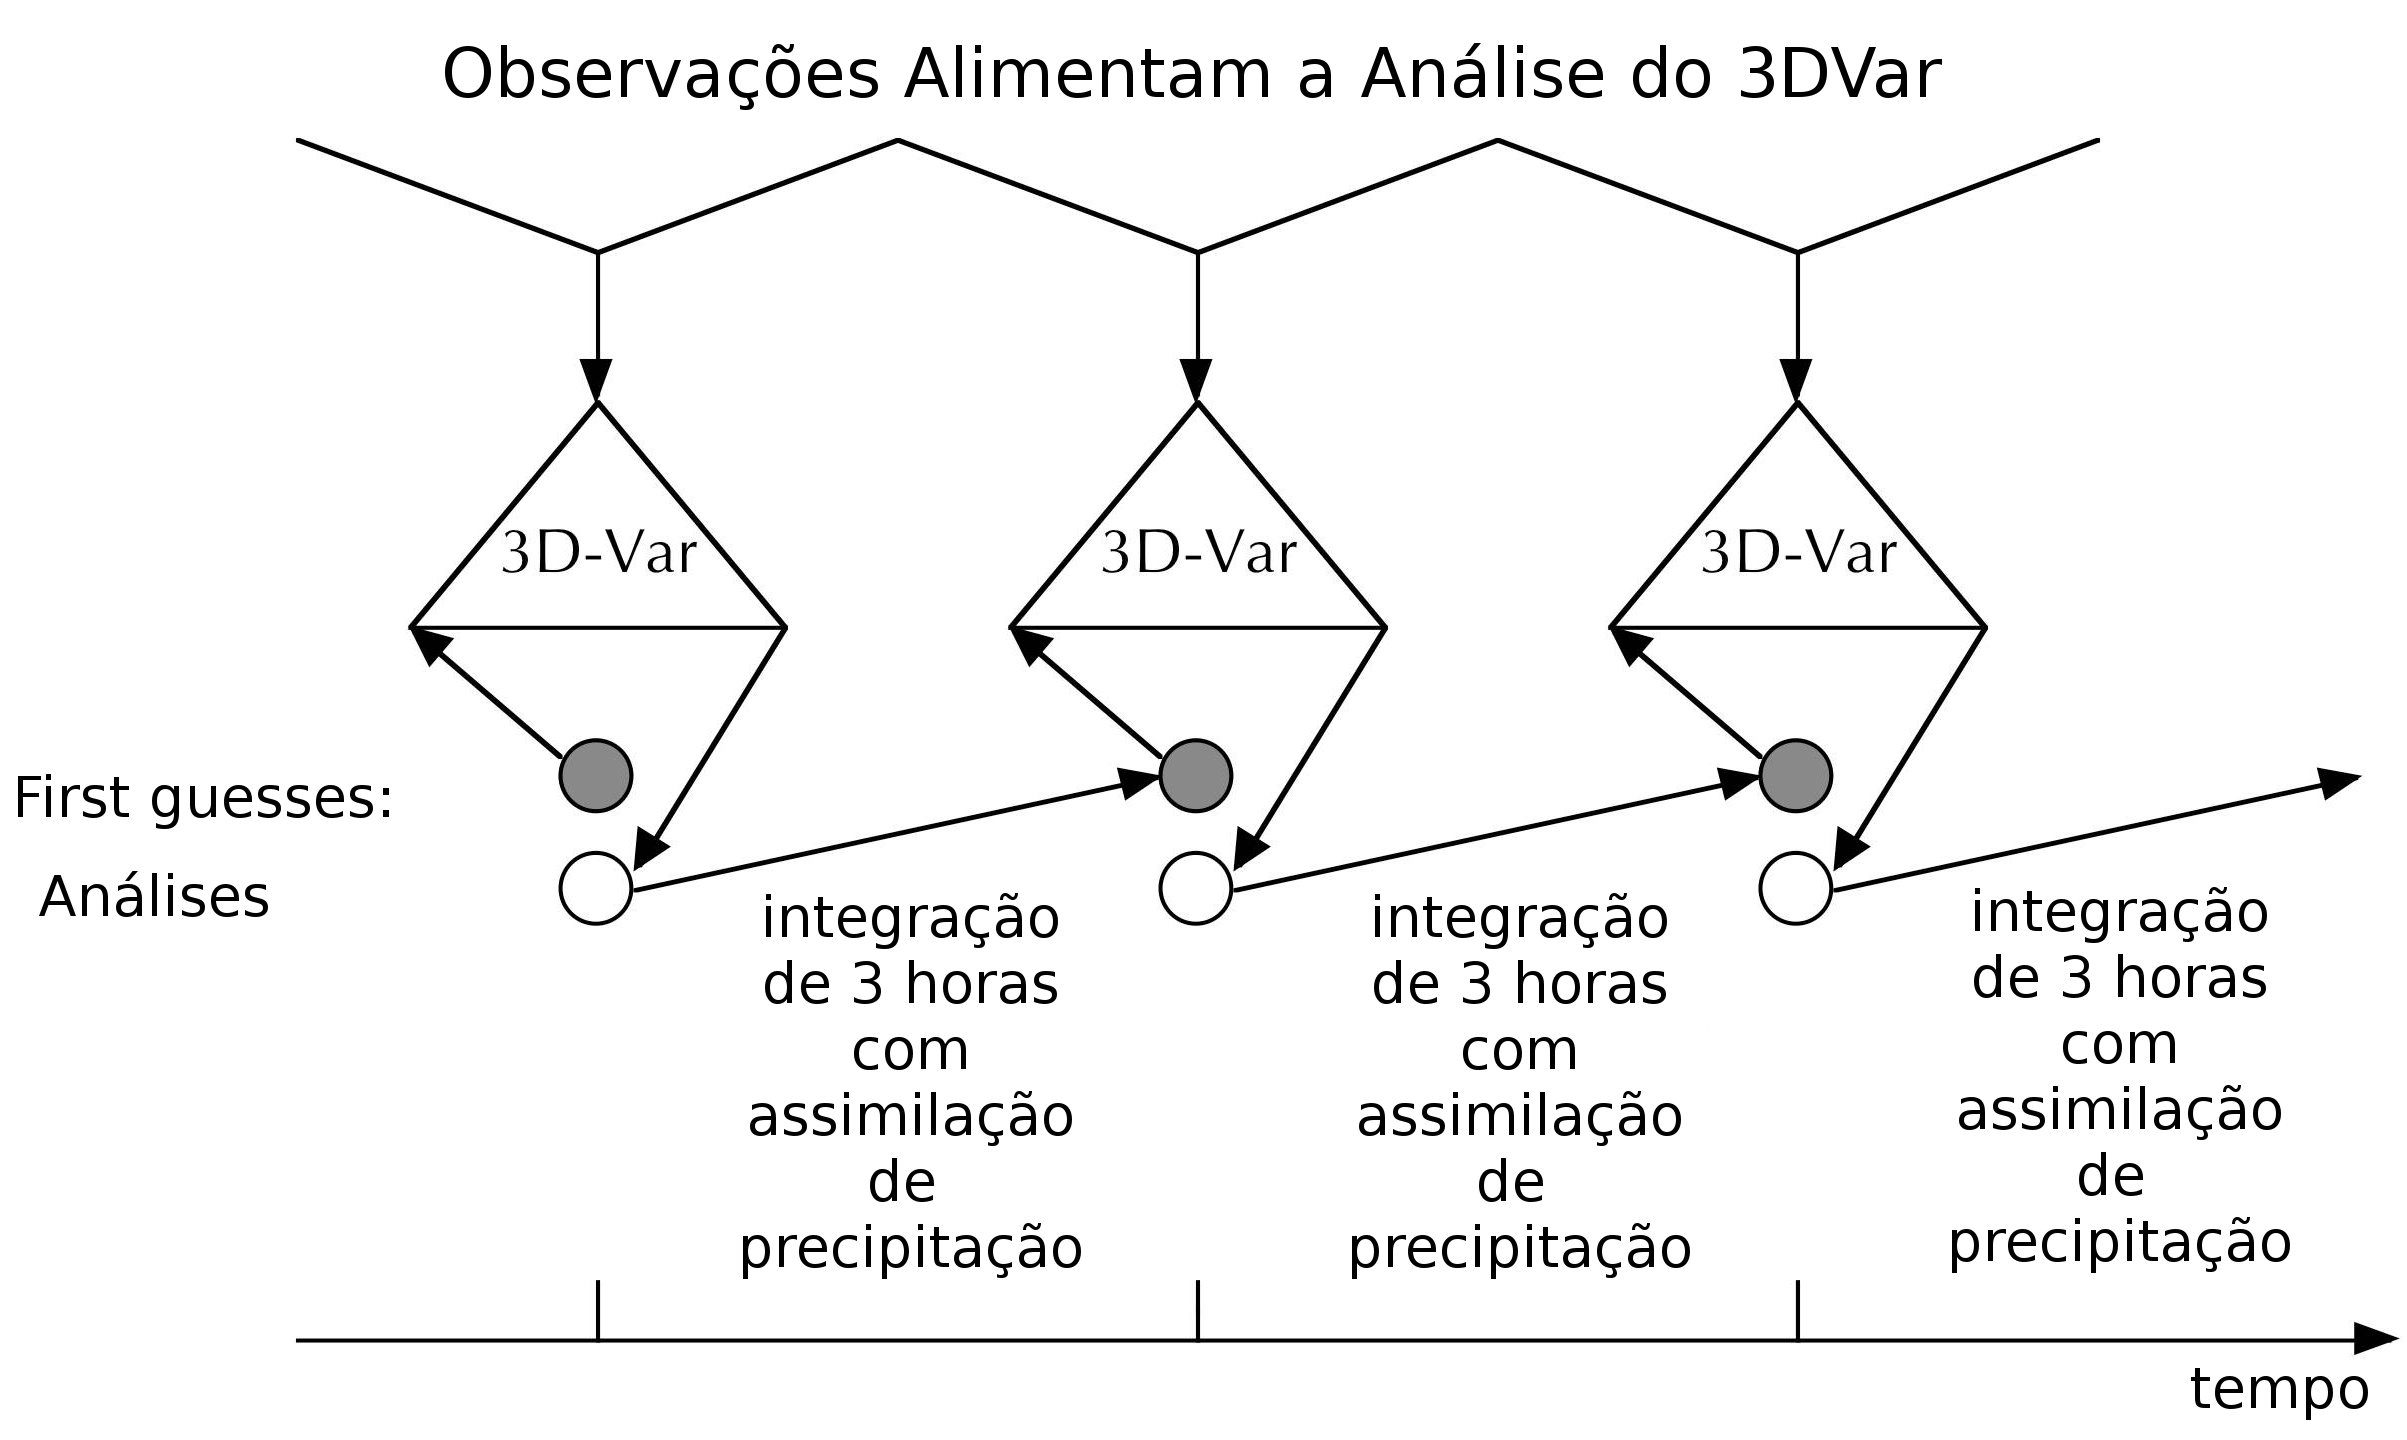
\includegraphics[height=7.5cm]{./figs/edas_pt.png}
\caption{Sistema de assimilação de dados EDAS/NCEP para um ciclo de 12Z.}
\FONTE{Adaptado de \citeonline{messingeretal06}}
\label{fig01}
\end{figure}

Sob este aspecto, geralmente nas primeiras horas de integração as variáveis dinâmicas estão se ajustando aos processos físicos/dinâmicos do modelo, isto é, as condições iniciais de superfície e atmosféricas estão entrando em balanço. Neste processo são filtradas as ondas espúrias (que são formadas a partir do desbalanço entre os campos de massa e vento do modelo) utilizando-se algum método de inicialização. Uma forma de se acelerar este processo de balanceamento, é incluir informações observadas e estimativas de superfície e/ou atmosfera, como precipitação, umidade e temperatura do solo. Isto faz com que seja reduzido o tempo de \textit{spin up} do modelo e permitindo que estas informações sejam propagadas pelo modelo ao longo do tempo de integração.

Tendo-se em vista que nas regiões tropicais do globo a convecção tem um papel dominante e sabendo-se que, em geral, os processos físicos associados à precipitação (convecção e microfísica) não são totalmente compreendidos, a modelagem atmosférica aplicada à estas regiões inclui uma série de aproximações. As parametrizações destes processos são inicialmente realizadas com estudos de campo que logo são \-mo\-de\-la\-dos e então, extrapolados para o globo todo. Outros fatores como interações não lineares (principalmente sobre continente) com processos de superfície e camada \-li\-mi\-te, tornam difícil a previsão da precipitação. Consequentemente a convecção tende a não se formar nos horários e locais previstos por um \-mo\-de\-lo de mesoescala (como é o caso do modelo Eta). Por isso, estudos têm sido realizados com foco nas regiões tropicais com o objetivo de tentar minimizar os efeitos destas aproximações e/ou contorná-las. Uma forma de se atenuar este problema é incluir a precipitação no ciclo de assimilação de dados.

Diferentemente da IF, que se utiliza da inversão da parametrização convectiva para a assimilação da precipitação, a inclusão da precipitação no ciclo de assimilação de dados realizada neste trabalho é similar à técnica de \textit{nudging} em que as quantidades de umidade e temperatura são modificados à partir da comparação da precipitação produzida pelo modelo de previsão com a precipitação estimada/observada \cite{carrbaldwin91}. Além disso, uma das vantagens desta técnica está na sua implementação que não requer a modificação das equações prognósticas do modelo, pela inclusão de um termo extra para realizar o \textit{nudging} e também pode ser aplicada em conjunto com vários tipos de parametrização convectiva \cite{rogersetal05}.

\section{Área de Estudo}

A maior parte da AS está situada em uma área tropical extremamente chuvosa onde o potencial hídrico é um dos maiores do mundo. A precipitação exerce grande influência em diversos setores da atividade humana, como o planejamento agrícola, energético e hídrico, além de ser um fator determinante do clima e do tipo de ve\-ge\-ta\-ção característicos de diversas regiões. Além disso, o excesso e a escassez de precipitação podem proporcionar graves consequências à população, como episódios de enchentes e secas intensas, os quais acarretam perdas humanas e prejuízos materiais. Dessa forma, conhecer sua distribuição e quantidade sobre uma determinada área ou região, é crucial para melhorar o entendimento do ciclo hidrológico e de sua interação com as atividades do homem.

A AS – região de estudo deste trabalho, está situada entre os oceanos Pacífico e Atlântico e meridionalmente entre as latitudes de 10$ºN$ e 60$ºS$. Esta é uma região sobre a qual atuam diversos tipos de sistemas atmosféricos reguladores do tempo e do clima e que têm importância devido à sua interação com a precipitação e a liberação de calor latente. Dentre eles, pode-se citar: a Zona de Convergência do Atlântico Sul (ZCAS), Zona de Convergência Intertropical (ZCIT), Jatos de Baixos e Altos Níveis, Alta da Bolívia e a Baixa do Chaco. Além disso, massas de ar e frentes atmosféricas entram e saem com frequência do continente. O deserto do Atacama, a cordilheira dos Andes, a floresta Amazônica e o Nordeste brasileiro, são exemplos também dos diferentes tipos de climas e regiões presentes na AS - \autoref{fig02}. Toda essa variedade de sistemas ambientais e meteorológicos em um continente situado numa zona tropical do globo, é consequência direta dos diferentes regimes de precipitação presentes na região. Além disso, há que se considerar também que, pelo fato de a AS estar situada no Hemisfério Sul (HS), as porções de terras e continentes nesta parte do globo são menores do que as porções de mares e oceanos. Esta situação é contrária ao que ocorre no Hemisfério Norte (HN). Nesta parte, a cobertura de radiossondagens e de equipamentos de monitoramento atmosférico sobre os continentes é muito maior e eficaz. Sobre o HS, este tipo de situação implica diretamente no uso de mais dados de satélites do que de observação em superfície.

\begin{figure}[!h]
\centering
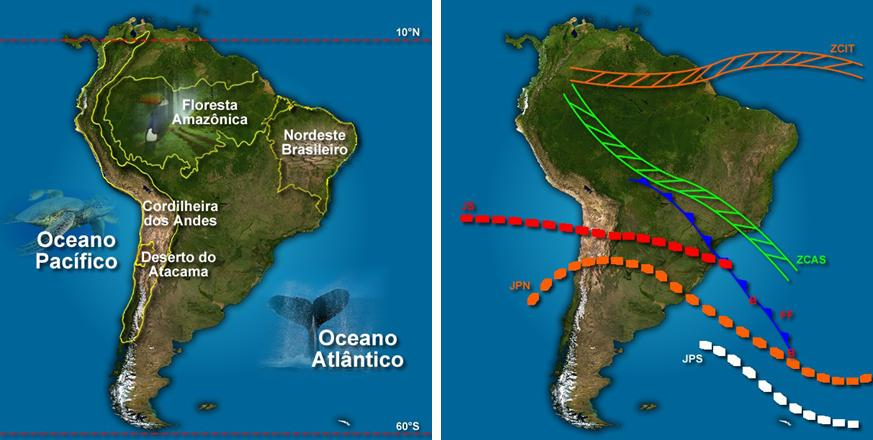
\includegraphics[height=7.5cm]{./figs/fig02.png}
\caption{As diferentes regiões e sistemas atmosféricos da América do Sul.}
\FONTE{Adaptado de \citeonline{satyamurtyetal98}}
\label{fig02}
\end{figure}

Grande parte dos regimes de chuva observados sobre os trópicos e em especial sobre a AS, é proveniente de um conjunto de sistemas meteorológicos denominados Sistemas Convectivos de Mesoescala (SCMs). Os SCMs são importantes fenômenos meteorológicos cuja principal característica é a sua organização em diversas formas, mas com escala espacial da ordem de centenas a milhares de quilômetros de extensão. Os Complexos Convectivos de Mesoescala (CCMs) são uma classificação dos SCMs e representam sistemas convectivos que produzem alterações significativas na dinâmica de mesoescala, sendo na geração e distribuição de calor latente, nas alterações de estabilidade vertical e redistribuição de umidade e, principalmente, na quantidade de radiação que entra e sai da atmosfera, devido à cobertura de nuvens associados a esses sistemas \cite{velascofritsch87}.

Diversos autores como \citeonline{menezessilvadias04}, \citeonline{herdiesetal07} e mais recentemente \citeonline{rozantecavalcanti07}, realizaram estudos numéricos sobre a simulação de CCM sobre a América do Sul, especialmente à leste dos Andes sobre o norte da Argentina. Nestes estudos, além da quantificação e determinação da climatologia dos CCMs sobre a AS, avaliou-se o impacto da assimilação de dados do projeto de campo do SALLJEX na simulação de sistemas convectivos de mesoescala. Também  se procurou as configurações mais adequadas para a simulação dos CCMs sobre o norte da Argentina. Estes tipos de estudos tem sua importância devido ao fato de que os CCMs são importantes fenômenos meteorológicos causadores de tempo e clima severos e que contribuem significativamente para a variação dos níveis pluviométricos, principalmente sobre as regiões tropicais e que podem estar associados a chuvas muito fortes, intensas rajadas de ventos, descargas elétricas atmosféricas, granizo e até tornados \cite{maddox80}; \cite{menezessilvadias04}.

Historicamente, a primeira definição formal de CCM foi introduzida por \citeonline{maddox80} para o Hemisfério Norte (HN). Mais tarde outros autores utilizaram esta definição para estudar outros casos de CCMs em partes diferentes do globo, como \citeonline{velascofritsch87}, na América do Sul. Segundo os critérios de \citeauthoronline{maddox80}, os CCMs podem ser classificados de acordo com suas características físicas: forma, tamanho e ciclo de vida. Quanto à forma, o CCM deve ser de formato circular, com excentricidade maior do que 0,7 (considerando-se a razão entre o eixo menor e o eixo maior - \autoref{fig03}). Quanto ao tamanho, o CCM deve apresentar uma cobertura de nuvens com temperaturas no infravermelho menores do que -32$ºC$ e com área de 100.000 $km²$. Na região mais interna da nuvem, as temperaturas devem ser mais frias (menores do que -52$ºC$) e com área em torno de 50.000 $km²$. Quanto ao ciclo de vida, o CCM deve apresentar as características de tamanho persistentes a um período superior a 6 horas.

\begin{figure}[!ht]
\centering
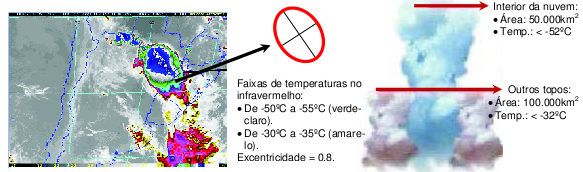
\includegraphics[height=4.5cm]{./figs/fig08.png}
\caption{À esquerda: imagem no infravermelho do satélite GOES (20030123, às 02:09 UTC). Ao centro: característica da excentricidade do CCM ocorrido nesta data. À direita: secção transversal de uma nuvem do gênero \textit{Cumulonimbus} durante um CCM.}
\FONTE{\citeonline{rozante08}}
\label{fig03}
\end{figure}

Todas estas características são semelhantes em escalas espaciais meso-a (ou meso-$\alpha$, de 250 a 2500 $km$ de extensão e escala de tempo de 6 horas) e meso-b (ou meso-$\beta$, de 25 a 250 $km$ de extensão e escala de tempo inferior a 6 horas).

Tipicamente, os CCMs são caracterizados por um conjunto de nuvens do gênero \textit{Cumulonimbus} cobertas por uma camada densa de nuvens do gênero \textit{Cirrus} e são facilmente identificados em imagens de satélites \cite{silvadias87}. O ciclo de vida dos CCMs é habitualmente noturno, ou seja, sua máxima extensão ocorre durante a madrugada \cite{velascofritsch87}, sendo o fim desse ciclo na metade do dia subsequente. Estas características dos CCMs tropicais e subtropicais são semelhantes em ambos os hemisférios (HN e HS) e estão sumarizadas na \autoref{tab01}.

\begin{table}[!h]
\caption{Resumo das Características dos CCMs.}
\label{tab01}
\centering
\begin{tabular}{c|p{12cm}l}
\hline
\multicolumn{2}{c}{Caractarísticas}                                                 \\
\hline
Forma                                       & Circular: excentricidade maior do que 0,7.\\
\hline
\multirow{4}{2cm}{Tamanho}                  & Nuvens: topo com temperaturas \\
                                            & inferiores a -32$ºC$ e cobertura \\
                                            & com área de $\sim$ 100000 $km²$; \\
                                            & Parte interna: temperaturas inferiores a -52$ºC$ e área de 50000 $km²$.         \\
\hline
\multirow{3}{2cm}{Ciclo de Vida}            & As características do tamanho devem persistir por mais do que 6 horas;   \\
                                            & Habitualmente noturno, com máxima extensão na madrugada.                \\
\hline
\multirow{3}{2cm}{Escala}                   & Meso-$\alpha$: 250 a 2500 $km$ de extensão e duração igual ou superior a 6 horas;      \\
                                            & Meso-$\beta$: 25 a 250 $km$ de extensão e duração inferior a 6 horas. \\
\hline
\multirow{4}{2cm}{Locais de Ocorrência} & Estados Unidos (HN);                  \\
                                            & Pacífico Oeste (HN);              \\
                                            & África (HS);                      \\
                                            & América do Sul (HS);              \\
\hline
\end{tabular}
\FONTE{Adaptado de \citeonline{velascofritsch87}}
\end{table}

No Brasil os CCMs ocorrem mais frequentemente sobre a região Sul, havendo também referências de se deslocarem para as regiões Sudeste e Centro-Oeste, podendo ocorrer em todas as estações do ano \cite{silvadias96}.

Na AS, o principal mecanismo de transporte de umidade da região amazônica para a região sul da AS, é o JBN. O JBN é frequentemente associado ao transporte de umidade e consequente formação da convecção de grande parte dos SCMs \cite{ferreiraetal03} que ocorrem sobre a região centro-sul da AS. O transporte de umidade da região amazônica em direção à região sul da AS, geralmente condensa e precipita na região de saída do JBN, produzindo fortes correntes descendentes sob o núcleo dos SCMs, com o máximo de precipitação durante a noite \cite{noguesetal00}. Esta característica é predominante em meses de verão, sendo que em meses de inverno, boa parte da umidade que condensa e precipita sobre o sul do continente é transportada pelos ventos alísios no norte do nordeste do continente. Na \autoref{fig04} é mostrado um modelo conceitual dos JBN e sua associação com a formação dos CCMs \cite{marengoetal04}.

\begin{figure}[!h]
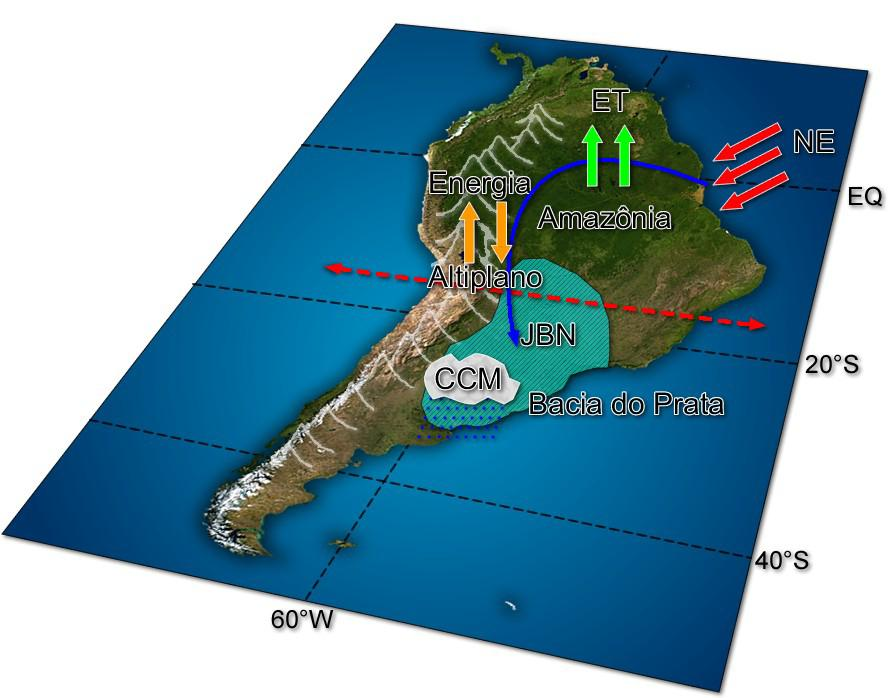
\includegraphics[height=10cm]{./figs/fig10.png}
\caption{Modelo Conceitual dos JBN. Na figura: ET - Evapotranspiração; JBN - Jato de Baixos Níveis e CCM - Complexo Convectivo de Mesoescala; NE - Ventos Alísios.}
\FONTE{adaptado de \citeonline{marengoetal04}}
\label{fig04}
\end{figure}

Portanto, para prever e simular as alterações dinâmicas e atmosféricas causadas por esses sistemas convectivos tais como as mudanças de fase da água, os efeitos dos processos radiativos (de onda curta e longa), as trocas turbulentas de calor, \textit{momentum} e vapor d'água entre a superfície e a atmosfera e os transportes turbulentos de calor, umidade e \textit{momentum} na atmosfera, exigem não apenas modelos modernos e computadores de alto desempenho, mas principalmente o aprimoramento do uso das observações disponíveis para que a condição inicial dos modelo de PNT seja a mais realística possível e, com essa análise mais acurada, fazer estudos diagnósticos que permitam o entendimento da dinâmica dos mesmos.

\break

\section{Objetivos}
\label{ss:objetivos} 

O objetivo principal deste trabalho é avaliar o impacto da inclusão de dados de precipitação no sistema de assimilação de dados regional do CPTEC.

Além disso, como objetivos específicos, buscou-se avaliar também:

\begin{enumerate}
\item O impacto da assimilação de dados de precipitação no desempenho do modelo Eta durante o mês de Janeiro de 2003;
\item O impacto da assimilação de dados de precipitação em um estudo de caso de CCM ocorrido em janeiro de 2003: identificação e simulação (ciclo de vida, posicionamento e intensidade);
\end{enumerate}

Para este propósito foi utilizado o sistema de assimilação de dados RPSAS junto com o modelo regional de mesoescala Eta. Dados de precipitação provenientes do \textit{Tropical Rainfall Measuring Mission} (TRMM) foram usados neste estudo. Esta avaliação teve também o intuito de verificar como a assimilação de precipitação no sistema Eta+RPSAS melhora a qualidade das análises e previsões regionais. O estudo foi desenvolvido para o mês de janeiro de 2003, período em que se têm dados observados do SALLJEX, com especial atenção ao período em que houve ocorrência dos CCM (18 a 23 de janeiro de 2003).

No \autoref{ss:cap2} deste trabalho são apresentados os componentes do sistema de assimilação de dados RPSAS que foram utilizados nos experimentos, considerando-se também as principais características do modelo Eta, método de assimilação e o conjunto de dados utilizado. No \autoref{ss:cap3} apresentam-se os resultados do período de análise, avaliação do desempenho do sistema Eta+RPSAS e o impacto da assimilação de  precipitação nas previsões do modelo Eta. No \autoref{ss:cap4} apresenta-se um estudo de caso de CCM. Finalmente, no \autoref{ss:cap5}, são apresentadas as conclusões e sugestões de trabalhos futuros.

%% CAPITULO 2
\hypertarget{estilo:capitulo}{}
\chapter{DADOS E METODOLOGIA}
\label{ss:cap2}

\section{Dados}
\label{ss:dados}
    
Para o período de estudo deste trabalho foram utilizados dados observados de precipitação provenientes de estações de superfície e dados estimados de satélites meteorológicos. Estes dados foram utilizados para a elaboração dos campos iniciais de precipitação, utilizados na assimilação pelo modelo Eta e na avaliação dos resultados. Adicionalmente dados das reanálises do CPTEC e do NCEP/DOE foram utilizados também para comparações e verificações do desempenho do sistema Eta+RPSAS com e sem a inclusão da precipitação estimada. Nos tópicos a seguir, apresenta-se uma breve descrição desses conjuntos de dados.

\subsubsection{\textit{Tropical Rainfall Measuring Mission} (TRMM)}

O satélite TRMM foi lançado em 27 de novembro de 1997 e é um projeto de parceria entre a NASA e a \textit{Japan Aerospace eXploration Agency} (JAXA), tendo como missão principal  fornecer informações sobre a estrutura e a distribuição espacial da preci-pitação, sua influência no clima das regiões tropical e subtropical e sua importância no ciclo hidrológico \cite{simpsonetal88}; \cite{simpsonetal96}.

O TRMM possui órbita polar com 35° de inclinação a 450 $km$ de altura, com alta resolução temporal (possui um período de translação de apenas aproximadamente 90 minutos e 16 órbitas por dia) varrendo as faixas de latitudes tropicais (50$ºN$ e 50$ºS$). Além disso, o TRMM é equipado com sensores específicos para o estudo da precipitação possibilitando a aquisição de informações sobre a precipitação tropical, relâmpagos e sobre a energia radiante das nuvens e da superfície terrestre. Estes sensores incluem:

\begin{itemize}
\item Imageador de microondas (TMI);
\item Radar de precipitação (PR);
\item Radiômetro no visível e no infravermelho (VIRS);
\item Sensor de energia radiante da superfície terrestre e das nuvens (CERES);
\item Sensor para imageamento de relâmpagos (LIS).
\end{itemize}

Além disso, as estimativas de precipitação são validadas em superfície através de um programa em paralelo denominado \textit{Groud Validadtion} (GV) que conta com uma série de radares meteorológicos em superfície espalhados ao longo da faixa intertropical \cite{collischonnetal07}.

Os dados estimados de precipitação provenientes do TRMM, que foram utilizados nos experimentos de assimilação deste trabalho, possuem resolução horizontal de 0.25° de latitude/longitude e frequência temporal de 3 horas. As estimativas de precipitação calculadas pelo TRMM são obtidas a partir do algoritmo 3B42 \cite{huffmanetal07}, utilizando informações sobre a estrutura vertical das nuvens. Estes dados encontram-se disponíveis em \url{ftp://trmmopen.gsfc.nasa.gov/pub/merged/combinedMicro}.
    
O algoritmo 3B42 é uma combinação de estimativas de precipitação por micro-ondas e infravermelho corrigidos através das informações sobre a estrutura vertical das nuvens, obtidas pelo radar de precipitação a bordo do satélite. O algoritmo para o cálculo das estimativas segue os seguintes passos:

\begin{enumerate}
\item Estima-se a precipitação com informações de dados de micro-ondas (TMI);
\item Estima-se a precipitação com informações do canal infravermelho (VIRS);
\item Calibra-se a precipitação estimada por micro-ondas e por infravermelho, disponibilizando-se as estimativas finais de precipitação a cada hora (em $mm/3h$).
\end{enumerate}

\subsubsection{\textit{South American Low Level Jet EXperiment} (SALLJEX)}

O SALLJEX foi um experimento de campo iniciado no centro-oeste da AS durante o período de 15 de novembro de 2002 a 14 de fevereiro de 2003 \cite{vera06}; \cite{herdiesetal07}. O programa \textit{South American Low-Level Jet} (SALLJ), um componente do programa \textit{Climate Variability and Predictability/Variabilty of the American Monsoon Systems} (CLIVAR/VAMOS), em linhas gerais, é um esforço coordenado internacionalmente para uma maior compreensão do papel que os JBN desempenham sobre a AS no transporte de umidade e nas trocas de energia entre os trópicos e extratrópicos, além da caracterização de aspectos da hidrologia regional, clima e variabilidade climática para a região de monção da AS \cite{herdiesetal07}.

Durante a campanha, uma grande rede de pluviômetros foi instalada entre os países Peru, Bolívia, Paraguai, Argentina e Brasil. Durante o período de observações, foram instaladas 22 novas estações de ar superior com 16 estações de balão piloto (PILOT) e 6 estações de radiossondagem (RAOB). Grande parte das estações RAOB foram operadas duas vezes ao dia (00Z e 18Z) enquanto que as estações PILOT foram \-o\-pe\-ra\-das quatro vezes ao dia (00Z, 06Z, 12Z e 18Z) durante um período de observações especial (denominado \textit{Special Observation Period} - SOP) entre 6 de Janeiro e 14 de Fevereiro de 2003. Durante o período de observações intensivas (denominado \textit{Intensive Observation Period} - IOP) grande parte das estações RAOB foram operadas de três a quatro vezes por dia enquanto que as estações PILOT foram operadas oito vezes ao dia em localidades específicas. A \autoref{fig05} mostra a distribuição espacial das radiossondagens e dos balões-piloto utilizados durante o período de estudos do SALLJEX na AS. 

As informações providas pelo experimento são de grande importância para a execução do presente trabalho, pois representam dados de superfície e de radiossondagem (com 1º de resolução espacial) que serão utilizados para a avaliação dos processos de assimilação com o sistema de assimilação de dados RPSAS do CPTEC. Os dados da campanha SALLJEX utilizados neste estudo podem ser obtidos em \url{http://data.eol.ucar.edu/master_list/?project=SALLJEX}.

\begin{figure}[!hpb]
\centering
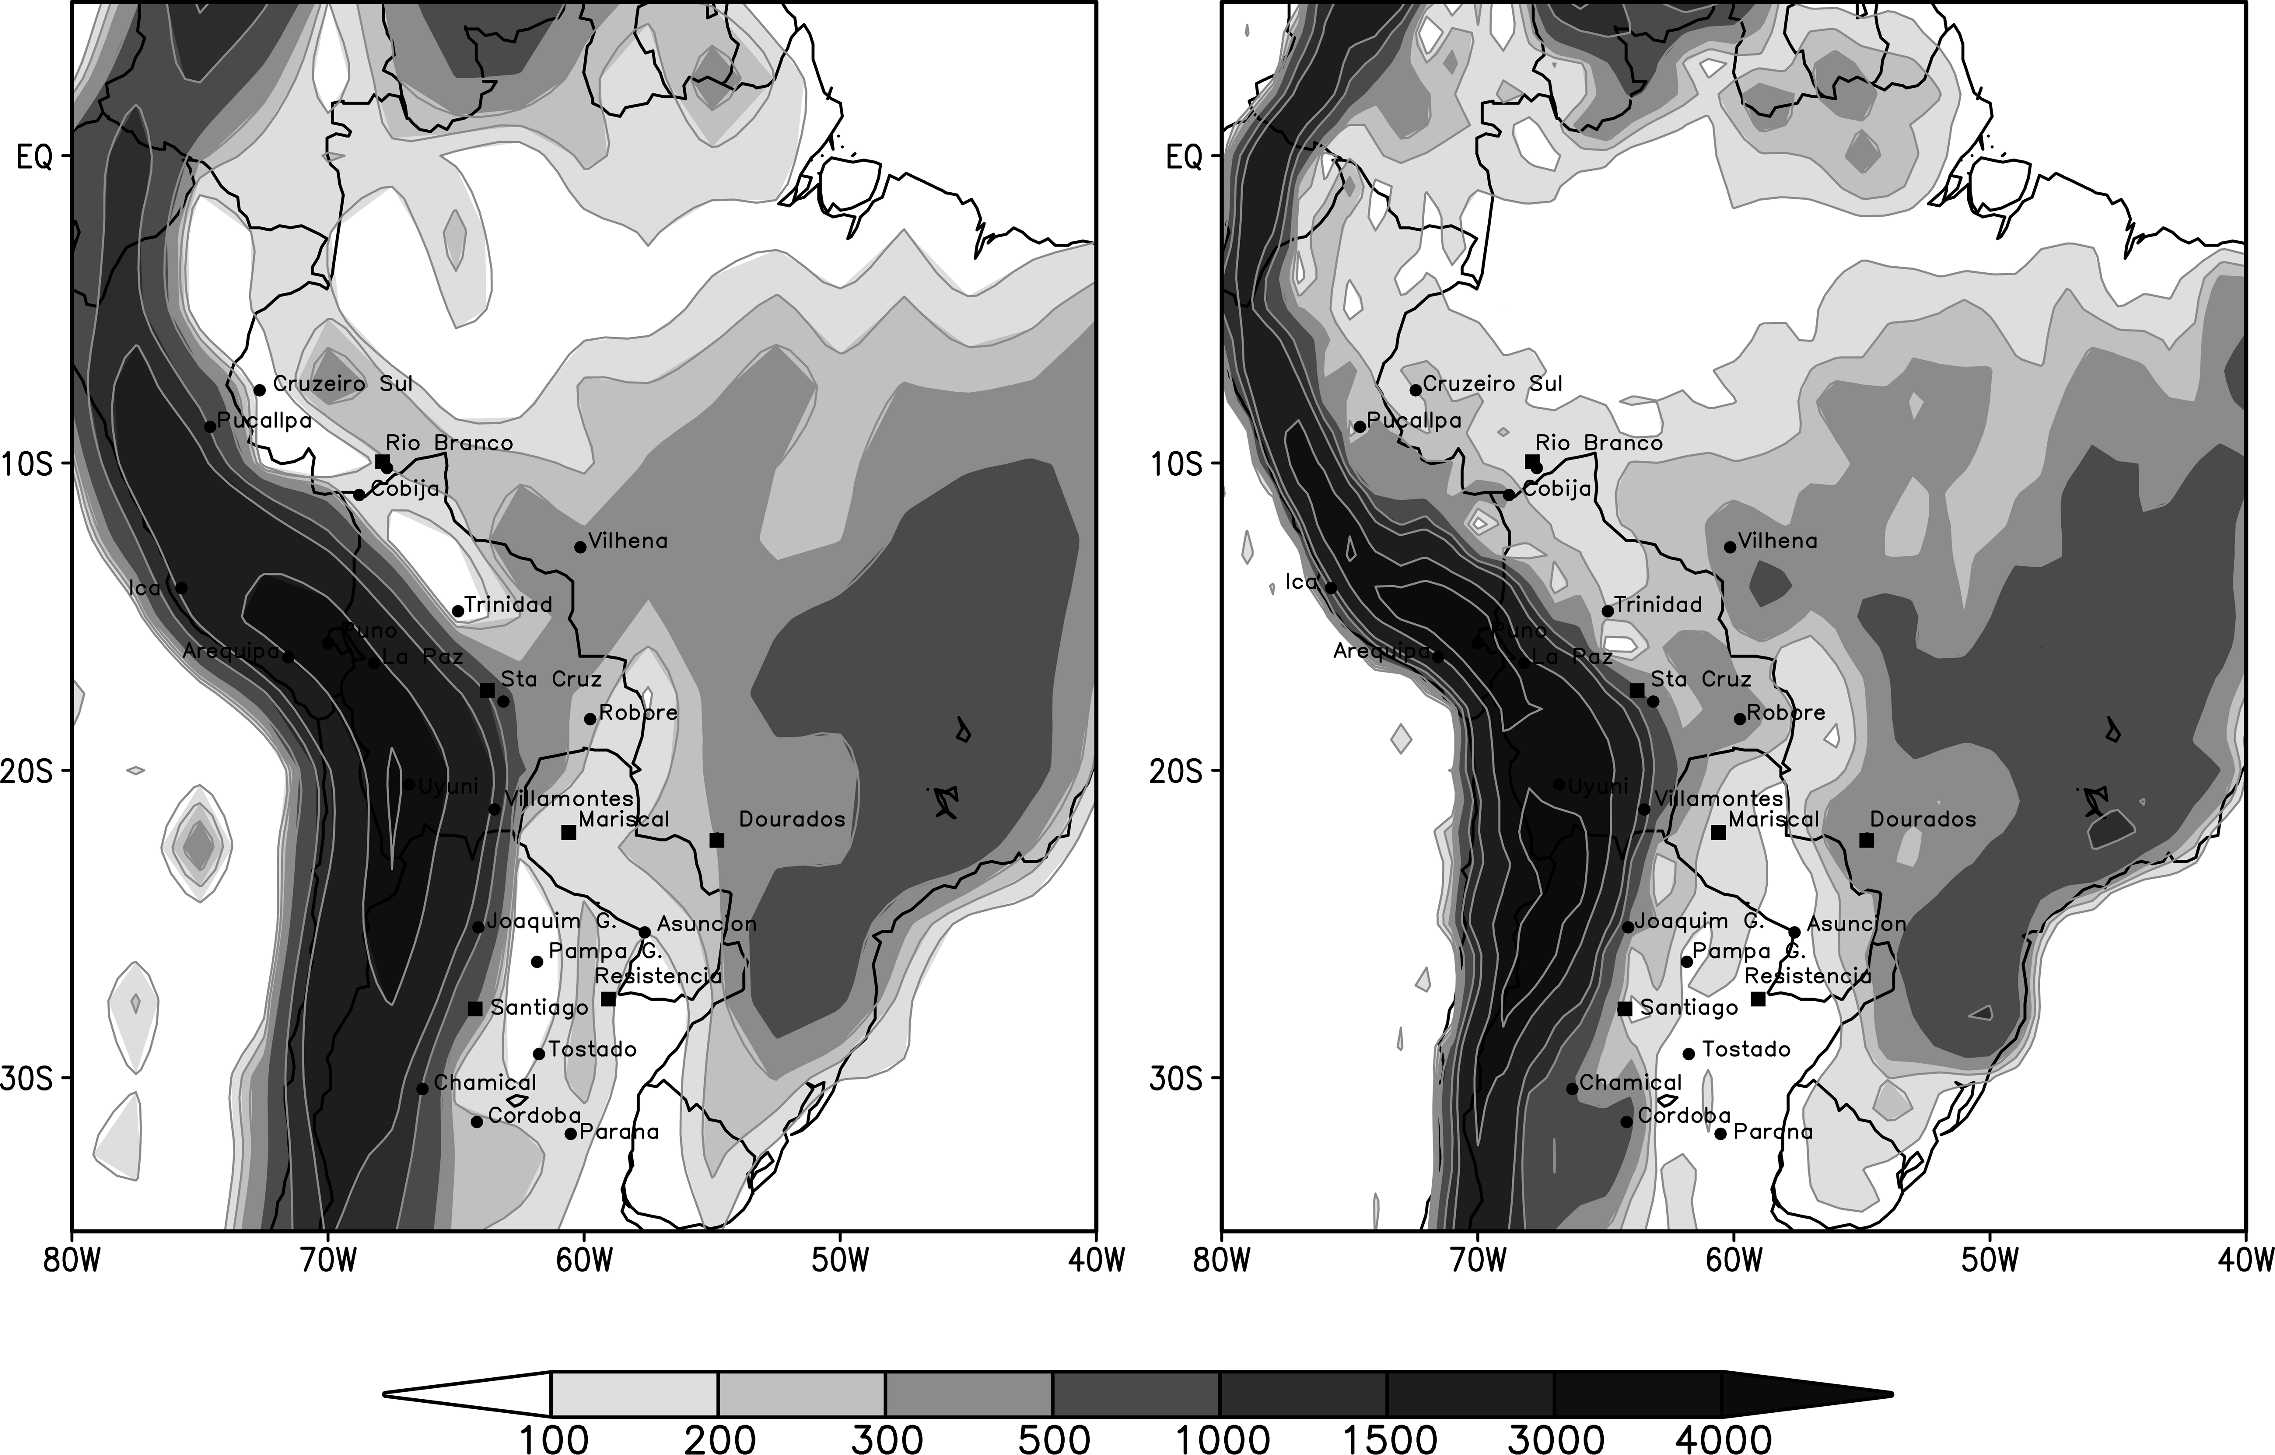
\includegraphics[height=7.5cm]{./figs/rede-salljex.png}
\caption{Rede de radiossondas do experimento SALLJ.}
\FONTE{\citeonline{herdiesetal07}}
\label{fig05}
\end{figure}

\subsubsection{\textit{Global Precipitation Climatology Project} (GPCP)}

O \textit{Global Precipitation Climatology Project} (GPCP) \cite{wcrp86} é um projeto internacional coordenado por diversas agências e centros meteorológicos ao redor do mundo. O objetivo do GPCP é caracterizar a precipitação global, desenvolvendo uma compreensão detalhada da distribuição espacial e temporal da precipitação.

Os dados de precipitação do GPCP representam estimativas diárias de precipitação com resolução espacial de 1º (versão 1.1, também denominada de \textit{One Degree Daily} - 1DD, \cite{huffmanetal97}) desde 1979 até o presente. Estas estimativas incluem dados de precipitação de mais de 6000 estações de superfície unidos a dados de satélites geoestacionários com dados obtidos a partir dos canais  infravermelho, microondas e microondas passivo. As estimativas diárias de precipitação podem ser obtidas em \url{ftp://rsd.gsfc.nasa.gov.br/pub/1dd-v1.1}

Uma das principais vantagens dos dados de precipitação do GPCP, além de sua alta resolução espacial, está na caracterização dos padrões de precipitação sobre os oceanos e o nível de detalhamento dos padrões de precipitação sobre os continentes. No entanto, a heterogeneidade das informações de precipitação que compoem o conjunto de dados do GPCP carece de maiores estudos de validação.

\subsubsection{Climatologia}

Para o cálculo do índice estatístico de Correlação de Anomalia (maiores detalhes no \autoref{apendice4}) foi necessário utilizar uma climatologia para o cálculo das anomalias dos experimentos e das reanálises. Esta climatologia foi feita com o modelo global do CPTEC T126L28 e interpolado para grade do modelo regional Eta de 20 $km$ \cite{sapucci09}. Para o cálculo desta climatologia, foram utilizadas como condição inicial as análises do NCEP.

\subsubsection{Reanálise Regional do CPTEC}
    
Para a comparação dos resultados obtidos a partir das simulações, foram utilizados os campos atmosféricos da reanálise do CPTEC \cite{aravequiaetal07} para o período do SALLJEX. A reanálise do CPTEC foi gerada com o sistema de assimilação de dados RPSAS com 40 $km$ de resolução espacial e 38 níveis verticais (versão 2003) e cobre o período de 1 de Janeiro de 2000 a 31 de Dezembro de 2004. Como condições de contorno, foram utilizadas as análises operacionais do modelo global do NCEP (T062L28). Nos experimentos da reanálise, foram geradas 4 análises diárias, nos horários das 00Z, 06Z, 12Z e 18Z e previsões diárias de 36 horas com saídas de 3 em 3 horas. 

Estes dados de reanálise são a combinação de dados observados com modelagem numérica e representam o estado da atmosfera mais próximo da observação para o período de estudos sobre a AS. O conjunto de análises da reanálise de 40 $km$ do CPTEC inclui perfis recuperados de temperatura e umidade (provenientes do ATOVS), dados de vento de satélites (CTW e \textit{Quick}SCAT), dados convencionais de superfície (SYNOP e BUOY) e dados de sondagens dos experimentos RACCI-LBA/2002 \cite{silvadiasetal03} além de dados do SALLJEX. Como produtos da reanálise do CPTEC, foram obtidas análises dos campos meteorológicos de variáveis comuns (prognosticadas e diagnosticadas pelo modelo Eta - ventos, temperatura, umidade, cobertura de nuvens etc), além de subprodutos espaciais, tais como campos climatológicos, médias diárias e mensais, precipitação diária, temperaturas má\-xi\-ma e mínimas entre outros. Estes produtos bem como os dados de reanálise produzidos pelo CPTEC, podem ser encontrados em \url{ftp://lba.cptec.inpe.br/lba_archives/PC/PC-404/regional_reanalysis}.

\subsubsection{Reanálise Global NCEP/DOE (versão 2)}

A Reanálise 2 do NCEP/DOE \cite{kanamitsuetal02} é a versão corrigida da Reanálise 1 do NCAR \cite{kalnayetal96} que tem como objetivo introduzir melhorias e correções. A Reanálise 2 do NCEP/DOE foi construída utilizando-se o modelo global T062L28 do NCEP e cobre o período de 1979 a 2009. Os dados da reanálise 2 do NCEP tem como principal objetivo fornecer informações mais acuradas sobre o passado utilizando dados de observação e modelagem numérica. As principais vantagens em se utilizar esta nova versão da reanálise em relação à sua versão anterior está na melhor representação do ciclo hidrológico, campos aprimorados de umidade do solo e temperatura à superfície, precipitação, cobertura de neve e outros.

Em \citeonline{kanamitsuetal02} são descritos alguns erros e deficiências encontrados durante o processo de obtenção da Reanálise 2 do NCEP/DOE. Dentre eles, a maioria por erros de programação, destacam-se os seguintes: as análises e o pós-processamento foram repetidos várias vezes durante a fase de produção; uso da climatologia sazonal média zonal do ozônio utilizada para o cálculo da radiação - a orientação latitudinal norte/sul foi invertida, o que pode causar erros no fluxo de radiação na estratosfera; erro de formulação do gradiente físico entre as camadas da superfície – que pode ocorrer sobre todo o globo e não apenas sobre os oceanos; erros de correção da umidade do solo quando este está saturado (ao invés de aplicar a correção de saturação do solo à segunda camada, esta foi aplicada à primeira); erros na redução da umidade do solo em casos em que a \-pre\-ci\-pi\-ta\-ção do modelo (ou ainda o \textit{run-off} do modelo) é menor do que a precipitação observada. Os dados da Reanálise 2 do NCEP/DOE podem ser encontrados em \url{http://www.esrl.noaa.gov/psd/data/gridded/data.ncep.reanalysis2.html}.

\subsection{Metodologia}

O Ciclo de Assimilação de Dados (CAD) do Centro de Previsão de Tempo e Estudos Climáticos (CPTEC) utilizado neste trabalho é composto de dois  componentes essenciais: o Controle de Qualidade (CQ) e o sistema regional de assimilação de dados RPSAS. A seguir é dada uma descrição sucinta destes dois componentes.

\textbf{a) Controle de Qualidade (CQ)}

Nesta fase é realizada uma depuração dos dados (observações) provenientes do \textit{Global Telecommunicatio System} (GTS) e de diversas outras fontes tais como o \textit{Internet Data Distribuition} (IDD), a Divisão de Satélites e Sistemas Ambientais (DSA/CPTEC), cooperações diretas com agencias espaciais e outros.

A checagem do controle de qualidade é feita em duas etapas: a primeira que abrange o desvio da observação em relação ao mesmo ponto dentro do campo de \textit{first guess} (que é denominado de \textit{background check}) e a segunda que aborda a consistência da observação em relação à sua vizinhança (denominada de \textit{buddy check}). No \textit{background check} as observações são rejeitadas ou assimiladas segundo um nível de tolerância determinado a partir das estatísticas de erro prescritas pelo sistema de análise. Caso o valor trazido pela observação esteja acima do nível tolerável, esta observação é rejeitada. Caso ele possua um desvio grande, mas dentro do nível de tolerância, essa observação é marcada como ``suspeita'' e, a partir daí procede-se ao \textit{buddy check}. No caso do sistema PSAS, este controle de qualidade é feito para as observações de ventos (componente zonal e meridional separadamente), altura geopotencial e umidade.

A partir disso, quando as observações são aceitas pelo sistema de assimilação, são calculadas diferenças entre os valores observados e estimados do \textit{first guess}. Estas diferenças são então utilizadas para a correção dos campos de previsão de curto prazo gerando a análise.  Maiores detalhes sobre o controle de qualidade do sistema de assimilação podem ser encontrados em \citeonline{andreolietal07}.

\textbf{b) Sistema de Assimilação de Dados}

A seguir são descritos de forma resumida os componentes do sistema de assimilação de dados RPSAS e como a é feita a inclusão da precipitação no sistema.

\textbf{b1) Análise – \textit{Regional Physical-space Statistical Analysis System (RPSAS)}}

O sistema de assimilação de dados \textit{Regional Physical-space Statistical Analysis System} (RPSAS) é a versão regional desenvolvida e mantida pelo CPTEC em parceria com o \textit{Global Modeling and Assimilation Office} (GMAO) da \textit{National Aeronautics and Space Administration} (NASA). O RPSAS utiliza o mesmo sistema de análise do \textit{Physical-space Statistical Analysis System} (PSAS) \cite{dasilvaetal95}; \cite{cohnetal98}. O RPSAS é considerado um esquema com características de Interpolação Ótima e de esquema variacional em três dimensões (3DVar), porém com a vantagem de ser independente do modelo não sendo necessária a linearização e a criação de modelos adjuntos para a assimilação (por se tratar de um sistema estatístico). Esse sistema de assimilação é utilizado de forma experimental com 20 $km$ de resolução espacial em conjunto com o modelo regional Eta principalmente para previsões de tempo de curto prazo (até 72 horas). O RPSAS é capaz de utilizar dados convencionais provenientes do GTS, tais como SYNOP, TEMP, SATOB entre outros, além de dados não convencionais de satélite (\textit{Quik}SCAT, TRMM, ATOVS, AIRS etc.).

O RPSAS utiliza como núcleo de análise o próprio PSAS, sendo que as equações de análise e inovação são resolvidas para o caso regional. Para calcular as inovações trazidas pelas observações e como forma de calcular a análise, são utilizadas as seguintes equações (adaptado de \citeonline{larsonetal98}):

\begin{equation}
(HP^{f}H^{T}+R)X=\textit{\textbf{w}}^o-H\textit{\textbf{w}}^f
\label{form01}
\end{equation}

\begin{equation}
\textit{\textbf{w}}^a-\textit{\textbf{w}}^f=P^{f}H^{T}X
\label{form02}
\end{equation}

Em que:

\begin{equation}
X^{a}=X^{b}+W[y^{o}-H(X^{b})]
\label{form03}
\end{equation}

Onde:

\begin{itemize}
\item $P^{f}$: é a matriz (de ordem $n$) de covariância dos erros da previsão;
\item $R$: é a matriz (de ordem $p$) de covariância dos erros de observação;
\item $H$: é uma matriz de ordem $p$$\times$$n$ que interpola as observações na grade no vetor previsão (em ponto de grade);
\item $\textit{\textbf{w}}^o$: é o vetor das observações, de ordem $p$;
\item $\textit{\textbf{w}}^f$: é o vetor previsão (em ponto de grade), de ordem $n$;
\item $\textit{\textbf{w}}^a$: é o vetor análise, de ordem $n$;
\item $\textit{X}$: é a matriz de covariância dos erros de observação.
\end{itemize}

O lado direito da \autoref{form01} é chamado de Vetor Inovação ou Resíduo Observação Menos Previsão (\textit{Observation Minus Forecast} - OMF), e o lado esquerdo da \autoref{form01} é chamado de Incremento da Análise (AI - \textit{Analysis Increment}). É importante observar que o PSAS ingere os dados observacionais através do vetor OMF na forma $\textit{\textbf{w}}^o-H\textit{\textbf{w}}^f$.

O PSAS resolve a \autoref{form01} e a \autoref{form02} sem formar explicitamente as matrizes $HP^{f}H^{T}$, $R$ e $P^{f}H^{T}$. A representação destas matrizes e a solução da \autoref{form01} e da \autoref{form02} podem ser encontradas em \citeonline{guoetal99}.

Em termos de custo computacional, como mencionado anteriormente, o PSAS é capaz de realizar os cálculos no ponto em que as observações se encontram. Considerando-se um sistema em que $n=10^{6}$ e $p=10^{5}$ (aproximadamente), arranjando-se e resolvendo-se a \autoref{form01}, o esforço computacional para o PSAS é reduzido pela metade (em relação ao 3DVar). O resto do tempo de máquina é devido à transformação da matriz $X$ (da \autoref{form02}) das observações para o espaço das observações \cite{cohnetal98}.

De forma simplificada, o PSAS segue o seguinte algoritmo:

\begin{enumerate}
\item Construção da matriz $HP^{f}H^{T}+R$ e solução da \autoref{form01} para $X$;
\item Construção da matriz $P^{f}H^{T}$ da \autoref{form02} e cálculo do incremento da análise ($\textit{\textbf{w}}^a-\textit{\textbf{w}}^f$) a partir de $X$;
\item Cálculo da previsão e da matriz dos erros de covariância das observações (matriz $X$) para uso nos passos \textit{a} e \textit{b};
\item Particionamento (tipagem) e outros processamentos nos dados observacionais de entrada.
\end{enumerate}

\textbf{b2) Previsão - Modelo Eta}

O modelo regional Eta \cite{mesingeretal88}; \cite{black94} utilizado nas \-si\-mu\-la\-ções é uma modificação da versão 2005 operacional do NCEP (a partir da qual também originou-se a versão \textit{Workstation}) em que foram implementadas algumas melhorias. Esta versão (pesquisa) foi escolhida para a realização dos experimentos por ser uma versão mais atual do modelo, que inclui um conjunto de física mais moderno e completo utilizada em modo pesquisa junto com o sistema RPSAS há alguns anos pelo grupo de AD do CPTEC. As principais diferenças entre as versões Eta Operacional e Eta Pesquisa estão sumarizadas na \autoref{tab02} a seguir.

\begin{table}[!hbp]
\caption{Diferenças principais entre os modelos Eta Operacional e Eta Pesquisa.}
\label{tab02}
\centering
\begin{tabular}{c|c|c|c}
\hline
Característica                       &                         & Eta Operacional              & Eta Pesquisa          \\
\hline
\multirow{2}{2.8cm}{Dinâmica}        &                         & \multirow{2}{2.8cm}{Hidrostática}      & Hidrostática       \\
                                     &                         &                   & Não-Hidrostática   \\
\hline
                                     & Superfície              & OSU LSM\footnotemark[1]          & NOAH LSM\footnotemark[2]          \\ 
\multirow{2}{2.8cm}{Parametrizações} & Precipitação Convectiva & Betts-Miller      & Betts-Miller-Janjić\\
                                     &                         &                   & Kain-Fritsh        \\
                                     & Microfísica de Nuvens   & Zhao              & Ferrier            \\
\hline
\end{tabular}
\end{table}

\footnotetext[1]{OSU LSM – \textit{Oregon State University Land Surface Model};}
\footnotetext[2]{NOAH LSM – \textit{Ncep, Oregon state university, Air force, Hydrologic research lab, Land Surface Model}.}

De forma geral, o modelo Eta se propõe a prever com detalhes sistemas organizados de mesoescala tais como CCM, Sistemas Frontais, Brisas Marítimas, Tempestades e outros \cite{chou96}. Como principais características, esta versão do modelo Eta pode ser utilizada nos modos hidrostático e não hidrostático (quando a escala dos movimentos horizontais é considerada maior do que a escala dos movimentos verticais) e com uma coordenada vertical eta que, em comparação à coordenada sigma, reduz os erros numéricos no cálculo da força do gradiente de pressão nas encostas de topografias íngremes. A \autoref{form04} define a coordenada vertical eta:

\begin{equation}
\eta=\frac{(p-p_{top})}{(p_{s}-p_{top})}\bigg[\frac{p_{ref}(z_{0})-p_{top}}{p_{ref}(z_{s})-p_{top}}\bigg]
\label{form04}
\end{equation}

Onde:

\begin{itemize}
\item $p$: é a pressão;
\item $p_{top}$: é a pressão no topo do modelo;
\item $p_{s}$: é a pressão na superfície;
\item $p_{ref}$: é a pressão de referência sobre uma superfície $\eta$ no topo de uma montanha ($z_{s}$) e na base da mesma ($z_{0}$).
\item $\frac{(p-p_{top})}{p_{s}-p_{top}}=\sigma$ (coordenada sigma)
\end{itemize}

O modelo utiliza uma grade horizontal do tipo semi-alternada E de Arakawa \cite{arakawalamb77} e um esquema de integração temporal \textit{split-explicit} - no qual os modos associados à gravidade são tratados com um passo de tempo menor, 20 $km$ de resolução espacial e 38 níveis verticais, com o topo do modelo a 25 $hPa$. Para uma melhor simulação dos processos próximos à superfície, o modelo possui 17 níveis verticais entre a superfície e o nível de 700 $hPa$. O domínio de integração do modelo regional cobre a maior parte da AS e parte dos Oceanos Atlântico e Pacífico, aproximadamente entre as latitudes de 10$ºN$ - 60$ºS$ e entre as longitudes de 90$ºW$ - 20$ºW$ \autoref{fig06}.

\begin{figure}[!h]
\centering
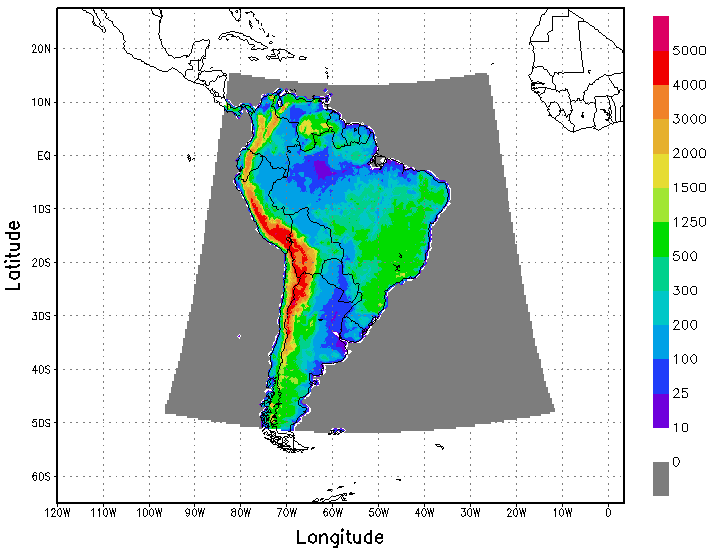
\includegraphics[height=8cm]{./figs/topo_dom.png}
\caption{Topografia e Domínio de Integração do modelo Eta.}
\label{fig06}
\end{figure}

\break

Em relação aos processos físicos, o modelo Eta pesquisa possui um conjunto de física completa com parametrização de convecção \textit{Cumulus} Betts-Miller modificado por Janjić (BMJ) \cite{betts86}; \cite{bettsmiller86}; \cite{janjic94}.



A parametrização BMJ considera apenas movimentos verticais ascendentes (convecção). O movimento convectivo transporta calor e umidade removendo ou reduzindo a condição de instabilidade da atmosfera (quando a atmosfera real é mais ou menos úmida do que a atmosfera de referência) alterando os perfis verticais de calor latente e umidade. A atmosfera de referência considera perfis de temperatura e umidade observados por \citeonline{betts86} e \citeonline{bettsmiller86}, que são relativamente secos e seguem adiabáticas úmidas. O esquema é acionado quando a atmosfera é mais úmida do que a atmosfera de referência (ambiente condicionalmente instável).

Outro aspecto relevante do modelo Eta pesquisa, é a parametrização de superfície. O esquema de superfície utilizado no Eta, inclui o modelo NOAH \cite{mitchelletal01}. Esta versão do NOAH utilizada em conjunto com o modelo Eta  inclui 16 classes diferentes de solo (entre 0 e 30 $cm$ de profundidade) e 24 classes diferentes de uso do solo (\textit{U.S. Geological Survey} - USGS \textit{landuse}) (\autoref{fig07}). As tabelas com os nomes das classes de solo e vegetação do NOAH LSM podem ser encontrada no \autoref{apendice1} deste trabalho (\autoref{tab05} e \autoref{tab06}).

\begin{figure}[!ht]
\centering
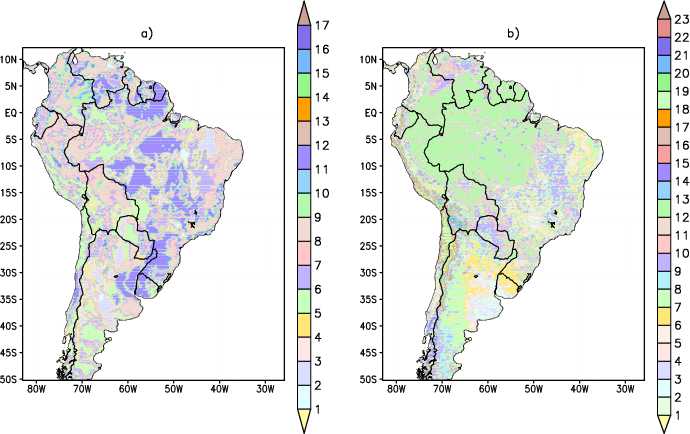
\includegraphics[height=8cm]{./figs/solo_veg_new.png}
\caption{a) Classes de Solo e b) Vegetação do Modelo de Superfície NOAH.}
\label{fig07}
\end{figure}

Entre outros aspectos da dinâmica e física do modelo, pode-se citar:
 
\begin{itemize}
\item Dinâmica: Hidrostática ou Não-Hidrostática – o modelo pode ser executado com a coordenada vertical sendo a pressão ou a altura, respectivamente;
\item Turbulência: Mellor-Yamada 2.5 para as trocas verticais na atmosfera livre (entre as camadas do modelo) e Mellor-Yamada 2.0 para as trocas entre a superfície e a camada mais baixa do modelo \cite{melloryamada74};
\item Radiação: o cálculo da radiação de onda curta no modelo é baseado em \citeonline{lacishansen74} e \citeonline{felsschwarzkopf75} para o cálculo da radiação de onda longa;
\item Nuvens: esquema de microfísica de nuvens de Ferrier \cite{ferrieretal02}, onde podem ser estimadas nuvens altas, médias e baixas além de diversos tipos de hidrometeoros.
\end{itemize}

O albedo e fração de cobertura vegetal foram obtidos a partir de climatologias globais sazonais e mensais, respectivamente. As condições iniciais ($u$, $v$, $t$, $q$, $p_{s}$ - ventos temperatura, umidade e pressão à superfície) no primeiro ciclo de assimilação foram provenientes da análise do NCEP, e fornecidas posteriormente pelo processo cíclico de assimilação.  As condições de contorno foram geradas pelo modelo global T126L28 do CPTEC e atualizadas a cada 6 horas. A temperatura do mar foi obtida a partir dos valores semanais para o período de estudo com resolução 1º e mantidas constante durante o período de integração do modelo.

\textbf{b3) Assimilação de Precipitação}

No sistema de assimilação Eta+RPSAS foram ajustados os campos de temperatura e umidade do modelo seguindo o método de \citeonline{carrbaldwin91} através dos campos de precipitação estimada do TRMM (que foi considerada como precipitação observada para assimilação), durante o período da geração do \textit{first guess}, 6 horas antes da previsão de 24 horas como está esquematizado na \autoref{fig08}. Este processo foi iniciado sempre nos horários 00Z, 06Z, 12Z e 18Z.

\begin{figure}[!h]
\centering
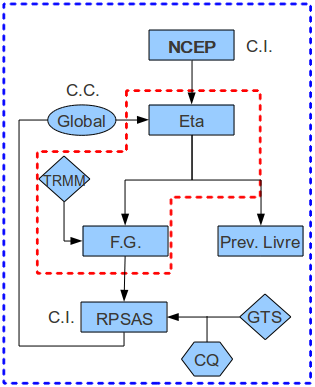
\includegraphics[height=10cm]{./figs/etarpsas2.png}
\caption{Ciclo de assimilação/previsão do sistema Eta+RPSAS/CPTEC. Na figura: CI: Condição Inicial; CC: Condição de Contorno; FG: \textit{First Guess} (previsão de 6 horas); CQ: Controle de Qualidade; GTS: \textit{Global Telecommunication System}.}
\label{fig08}
\end{figure}

Este método foi implementado no sistema de assimilação RPSAS por \citeonline{fernandez08}, seguindo basicamente o sistema de assimilação de dados EDAS do NCEP.

Para isso, em cada passo de tempo ($\sim$ 45 segundos) e em cada ponto de grade onde as observações de precipitação estão disponíveis, durante o período de geração do \textit{first guess}, compara-se a precipitação prevista ($P_{mod}$) com a precipitação observada ($P_{obs}$). Com isso, procede-se a uma avaliação da seguinte forma, como mostrado na tabela \autoref{tab03} \cite{linetal01}:

\begin{table}[!h]
\caption{Ajuste convectivo pelo método de Carr e Baldwin adaptado para o \-mo\-de\-lo Eta.}
\label{tab03}
\centering
\begin{tabular}{|c|c|c|c|}
\cline{3-4} 
\multicolumn{1}{c}{} &  & \multicolumn{2}{c|}{Ajustes}\tabularnewline
\hline 
\begin{sideways}

\end{sideways} &  & Ajusta-se $P_{mod}$ para 0; & \tabularnewline
\begin{sideways}

\end{sideways} &  & Ajusta-se o perfil de calor & \tabularnewline
\begin{sideways}

\end{sideways} & $P_{obs}=0$ & de acordo com $P_{mod}$; & Não é necessário fazer ajustes\tabularnewline
\begin{sideways}

\end{sideways} &  & Ajusta-se $q_{v}$ de forma que & \tabularnewline
\begin{sideways}

\end{sideways} &  & $RH$ permaneça inalterado. & \tabularnewline
\cline{2-4} 
\multirow{2}{0pt}{\begin{sideways}Condições\end{sideways}}
\begin{sideways}

\end{sideways} &  &  & Especifica-se uma camada\tabularnewline
 
\begin{sideways}

\end{sideways} &  & Multiplica-se o perfil de calor & vertical de nuvem baseada\tabularnewline
\begin{sideways}

\end{sideways} &  & latente do modelo por $\frac{P_{obs}}{P_{mod}}$; & em $P_{obs}>0$;\tabularnewline
\begin{sideways}

\end{sideways} & $P_{obs}>0$&  & Especifica-se um perfil\tabularnewline
\begin{sideways}

\end{sideways} &  & Ajusta-se $q_{v}$ de forma que & parabólico de calor latente;\tabularnewline
\begin{sideways}

\end{sideways} &  & $RH$ permaneça inalterado. & Especifica-se $RH$ na camada\tabularnewline
\begin{sideways}

\end{sideways} &  &  & de nuvem para 80$\sim$90\%.\tabularnewline
\hline
\multicolumn{1}{c}{} &  & $P_{mod}>0$ & $P_{mod}=0$ ou $P_{mod}<<P_{obs}$\tabularnewline
\cline{3-4} 
\multicolumn{1}{c}{} &  & \multicolumn{2}{c|}{Condições}\tabularnewline
\cline{3-4} 
\end{tabular}
\end{table}

\break

\begin{enumerate}
\item Se $P_{mod}>0$ e $P_{obs}=0$: toma-se novamente $P_{mod}$ e a quantidade correspondente de calor latente do modelo; ajusta-se a razão de mistura do vapor d'água ($q_{v}$) de forma que a umidade relativa ($RH$) permaneça inalterada; reduz-se a razão de mistura do vapor d'água para um valor além do necessário a fim de se proporcionar condições para produzir chuva ($q_{cmin}$);
\item Se $P_{mod}>P_{obs}>0$: reduz-se a liberação de calor latente em cada camada de precipitação através da multiplicação do perfil de calor latente pelo fator $\frac{P_{obs}}{P_{mod}}$; ajusta-se $q_{v}$ como no caso anterior, e nas camadas onde a precipitação começa a surgir, reduz-se a água da nuvem proporcionalmente, mas mantendo-se acima de $q_{cmin}$;
\item Se $P_{mod}<P_{obs}$: primeiro deve-se verificar se a convecção é possível, e caso seja positivo, diminui-se a escala de tempo convectiva a fim de se acelerar o processo de produção de precipitação convectiva; atingido este objetivo, uma quantidade de precipitação convectiva ($P_{cnv}$) se iguala à precipitação observada ($P_{obs}$) (mas não muito maior do que a quantidade máxima permitida pela parametrização convectiva).
\end{enumerate}

Depois do ajustamento convectivo, se $P_{cnv}<P_{obs}$ (neste caso, ou o perfil é não convectivo, ou a convecção máxima de precipitação é menor do que $P_{obs}$, procede-se a um ajustamento em escala de grade para a precipitação ($P_{grd}$) em função de $P_{obs}-P_{cnv}$.

Este procedimento é tal que:

\begin{enumerate}
\item Se $P_{grd}>0$: multiplica-se a escala de grade do perfil de calor latente pela razão $\frac{(P_{obs}-P_{cnv})}{P_{grd}}$, alterando-se $q_{c}$ nas camadas de produção de chuva pelo mesmo fator (mas mantendo-o acima do nível de $q_{cmin}$) e ajusta-se de tal forma que mantém-se inalterada;
\item Se $P_{grd}=0$: cria-se uma camada de nuvens (os limites superior e inferior da camada de nuvens são determinados pelo perfil de umidade do modelo e pela quantidade de precipitação da escala de grade) e o perfil parabólico de calor latente correspondente à produção de precipitação de escala de grade $(P_{obs}-P_{cnv})$. Dentro da camada de nuvem criada, $RH$ é ajustada para 80\% e $q_{c}$ é ajustada para um valor menor do que $q_{cmin}$.
\end{enumerate}

Inicialmente este sistema de assimilação de precipitação foi projetado para trabalhar com o modelo Eta do NCEP em conjunto com o sistema de assimilação de dados EDAS, utilizando uma análise que continha dados horários de observações de superfície (no caso, pluviômetros) e dados de precipitação obtidos a partir de vários sensores. Esta análise, na época, era conhecida por \textit{Stage IV Analysis} \cite{linetal01}. Desde 2001 quando o sistema de assimilação de precipitação foi implementada no EDAS do NCEP \cite{rogersetal01}, várias modificações foram feitas no modelo Eta e no sistema de assimilação EDAS e também no sistema de assimilação de precipitação, proposto anteriromente por \citeonline{carrbaldwin91}. Em 2005, o modelo Eta recebeu uma série de modificações (principalmente na parte física) e passou a ser denominado \textit{North American Model} (NAM) e, consequentemente, o sistema EDAS passou a ser denominado NAM \textit{Data Asimilation System} (NDAS). Dentre essas modificações que foram feitas no EDAS, na parte de assimilação de precipitação, está a adaptação do esquema de Carr e Baldwin de forma a funcionar com parametrizações físicas mais modernas, tornando essa parte do sistema mais independente do modelo Eta e da parametrização convectiva (\textit{Cumulus}) adotada. Esta modificação é que possibilitou a implementação do equema de assimilação de precipitação na versão do modelo Eta, implementada por \citeonline{fernandez08}. Em \citeonline{rogersetal05} são descritos com maiores detalhes as principais modificações e melhorias implementadas no sistema.

\subsection{Experimentos}

Com o intuito de se avaliar o impacto da assimilação de dados de precipitação do TRMM no sistema Eta+RPSAS, foram realizados os seguintes experimentos: um denominado SAP (Sem Assimilação de Precipitação) e outro denominado CAP (Com Assimilação de Precipitação). Em ambos os experimentos é feita a assimilação dos dados do GTS e ambos utilizam o Filtro Digital original do modelo Eta, sendo que a única diferença entre eles é a assimilação ou não da precipitação do TRMM. A \autoref{tab04} resume os experimentos realizados. No total foram idealizados seis experimentos sendo que apenas quatros foram realizados. Destes quatros apenas dois foram efetivamente utilizados para avaliação porque apresentaram resultados significativos. Dentre esses quatros experimentos, dois são os experimentos SAP e CAP e outros dois também foram sem e com a assimilação de precipitação, mas sem o FD. Em resultados preliminares foi encontrado que sem a inclusão do FD o modelo tornava-se instável e depois de poucas horas as integrações abortava, então se decidiu pela necessidade da inclusão do FD em todas as previsões. Neste caso, não investigou-se sobre o porquê deste tipo de comportamento do modelo com as configurações utilizadas. Os demais experimentos que compunham o conjunto dos seis, não foram finalizados porque faziam uso apenas da análise do NCEP como condição inicial, e, portanto, deu-se prioridade àqueles que utilizam como a análise gerada pelo RPSAS, tal como ocorre na operação do CPTEC.

\begin{longtable}{c|c|c|>{\centering}m{0.9in}|>{\centering}m{0.9in}|>{\centering}m{1in}}
\caption{Experimentos Realizados.}
\label{tab04}
\endfirsthead
\hline 
Nome & Dinâmica & C.I. & C.C. & Periodo & Descrição\tabularnewline
\hline 
SAP & Hidrostática & NCEP/Eta & Global T126L28 & 02-30 

Jan 2003 & Sem Precipitação\tabularnewline
\hline 
CAP & Hidrostática & NCEP/Eta & Global T126L28 & 02-30

Jan 2003 & Com Precipitação\tabularnewline
\hline
\end{longtable}

Nos experimentos, para o primeiro ciclo de assimilação/previsão, foi utilizada como condição inicial a analise do NCEP, e posteriormente a análise gerada pelo sistema RPSAS. Foram realizados ciclos de previsões às 00Z e 12Z gerando previsões diárias para 24 horas, com saídas a cada 6 horas Às 06Z e 18Z foram geradas apenas o \textit{first guess} utilizado nos horários subsequentes. Os experimentos foram realizados entre os dias 02 e 30 de Janeiro de 2003, utilizando-se o período de 2 a 15 Janeiro como período de \textit{spin up}. Este período de \textit{spin up} foi definido desta forma porque com a inclusão da precipitação no processo de assimilação/previsão ocorre um encurtamento do tempo necessário para que as condições iniciais do solo (temperatura e umidade) entrem em balanço e, 15 dias são suficientes para o \textit{spin up} de um modelo regional No entanto, um periodo mais longo - como um ou dois meses, pode também ser necessário dependendo do tipo de produto que se quer obter (reanálise ou análises/previsões). Logo, pode-se comparar o \textit{spin up} dos dois experimentos. Também foi idealizado utilizar-se o mês de dezembro de 2002 como período de \textit{spin up}, mas isto não foi feito porque a geração das analises pelo RPSAS exigiram recursos computacionais elevados.  Além disso muito mais espaço em disco seria necessário para armazenar as previsões do modelo global T126L28 do CPTEC. A \autoref{tab07} do \autoref{apendice3} apresenta o custo computacional demandado pelo sistema Eta+RPSAS para um experimento.

As análises geradas pelo RPSAS foram comparadas com as análises da Reanálise do CPTEC e Reanálise 2 do NCEP/DOE. Também as previsões do modelo Eta foram comparadas com os dados observacionais do SALLJEX e do TRMM.

Nos experimentos propostos, os campos iniciais de temperatura e umidade do solo foram obtidos a partir das análises globais do \textit{Global Forecast System} (GFS) do NCEP. Posteriormente, durante o processo cíclico de assimilação de dados, a temperatura e a umidade do solo foram calculadas pelo NOAH LSM a cada ciclo de previsão (\textit{first guess}). As condições de contorno foram provenientes das previsões do modelo global do CPTEC T126L28 e atualizadas a cada 6 horas. A temperatura do mar foi obtida dos valores semanais para o período de estudo com resolução 1º.

Nos experimentos as previsões foram inicializadas utilizando um Filtro Digital que segue o esquema proposto por \citeonline{lynchhuang93} com o objetivo de se acelerar o equilíbrio entre os campos de massa (componentes do vento) e os de velocidade (movimentos verticais) reduzindo o ruído gerado durante a integração do modelo. Em cada passo de tempo, e em cada ponto de grade, as variáveis prognosticas do modelo são filtradas obtendo-se, ao final do processo, uma Condição Inicial Filtrada (CIF). Esta CIF é a combinação das duas integrações feitas anteriormente (para frente e para trás). Em seguida, o modelo Eta utiliza esta CIF para fazer as previsões \cite{harter99}. Este procedimento foi realizado no início de cada previsão e depois da geração de cada análise. 

No modelo Eta, este filtro consiste em integrar o modelo por $N$ passos de tempo para trás e depois por $N$ passos de tempo para frente (totalizando $2N$ passos de tempo) a partir do início da previsão livre (00 h). Para o caso dos experimentos propostos, o valor de $N$ é 55 e o valor de $DT$ é 40 segundos (passo temporal). Com isso, a partir de $N$$\times$$DT$, obtém-se o valor de 2200 que é próximo àquele recomendado por \citeonline{pyle02}. De forma geral, o valor de $N$ deve ser calculado com base em $N$$\times$$DT$, cujo produto deve ser um valor não muito maior do que 2400 segundos. Valores altos de $N$ podem eliminar oscilações de baixa frequência e suavizar mais os campos prognósticos durante as 3 ou 6 primeiras horas de previsão \cite{pyle02}. No entanto, valores muito altos de $N$ podem também fazer com que o modelo torne-se muito instável comprometendo o processo de previsão. Uma tabela com diversos espaçamentos de grade e os correspondentes passos temporais pode ser encontrada em \citeonline{peters96}.

No \autoref{apendice2} são fornecidos maiores detalhes sobre os \textit{scripts} e sobre o desempenho computacional do sistema Eta+RPSAS implementado.

\subsection{Avaliação Estatística}
    
A destreza e a exatidão de um modelo de PNT é medida através de um conjunto de estatísticas que permitem, além de se avaliar as diferentes variáveis reproduzidas pelo modelo, identificar quais são as áreas do domínio que apresentam maior deficiência. Com a avaliação estatística, pode-se quantificar a destreza de um modelo de PNT segundo a sua habilidade nas previsões e observando-se o grau de realismo com que ele é capaz de simular um determinado evento atmosférico.
    
Para a avaliação espacial do desempenho do modelo foram aplicadas as seguintes estatísticas: o Viés, o Erro Quadrático Médio (EQM) e o Coeficiente de Correlação de Anomalia (CCA).

As estatísticas foram calculadas para a região à leste do Andes, sobre o norte da Argentina de coordenadas -72º$W$ a -48º$W$ e -33º$S$ a -18º$S$ (\autoref{fig09}).

\begin{figure}[!ht]
\centering
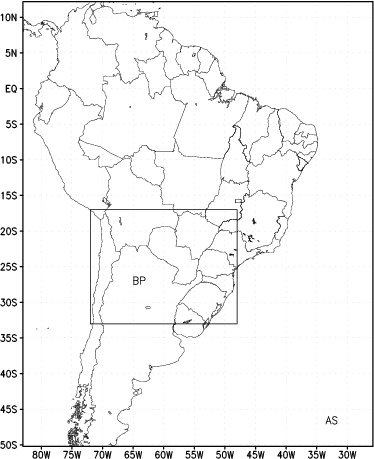
\includegraphics[height=9cm]{./figs/area_aval.png}
\caption{Área de avaliação utilizada no cálculo do Viés, EQM e CCA. BS: Bacia do Prata; AS: América do Sul.}
\label{fig09}
\end{figure}

No \autoref{apendice4} encontram-se as definições matemáticas dos diferentes índices utilizados.

%% CAPITULO 3
\hypertarget{estilo:capitulo}{}
\chapter{IMPACTO DA ASSIMILAÇÃO DE PRECIPITAÇÃO NO SISTEMA Eta+RPSAS}
\label{ss:cap3}

\section{Avaliação das médias dos experimentos durante Janeiro de 2003}
\label{ss:avalmedia}

Para se verificar o comportamento dos experimentos (sumarizados na \autoref{tab04}) ao longo do período de integração do modelo (de 02 a 30 de Janeiro de 2003), foi feita uma avaliação espacial e temporal média da integração do modelo durante o período de estudos em comparação com a Reanálise 2 do NCEP/DOE e a Reanálise do CPTEC. Para esta avaliação foram consideradas as análises do sistema RPSAS em um total de 113 análises (entre 00Z, 06Z, 12Z e 18Z, considerando-se também  o período de \textit{spin up}), a partir das quais foi feita a média espacial para o domínio de integração do modelo. Todos os campos considerados nesta avaliação espacial (incluindo-se a reanálise do CPTEC) foram interpolados para a grade da reanálise do NCEP utilizando-se a função \textit{lterp} do GrADS. 

Na \autoref{ss:avalprev} são apresentadas as séries de precipitação dos experimentos SAP e CAP e dos projetos GPCP, SALLJEX e TRMM (observações) e também as médias espaciais dos campos de precipitação dos experimentos e dos projetos. Em seguida na \autoref{ss:avaltempumi}, é feita uma análise média da temperatura e da umidade do solo do período. Na \autoref{ss:avalanl} é apresenta a avaliação espacial das Análises do sistema RPSAS contra as reanálises do CPTEC e do NCEP. Foram avaliadas as variáveis Temperatura, Ventos (componentes $u$ e $v$), Altura Geopotencial e Linha de Corrente nos níveis de 850, 500 e 250 $hPa$. Também, foram verificadas separadamente as componente zonal do vento ($u$) em 250 $hPa$ e meridional ($v$) em 850 $hPa$, além da Temperatura a dois metros. Na \autoref{ss:avalesanl} é feita uma avaliação do Viés e do Erro Quadrático Médio das séries das análises do RPSAS contra a reanálise do NCEP para o período de estudos.

\subsection{Avaliação das Previsões (Previsões Eta X Observações)}
\label{ss:avalprev}

Neste tópico é feito uma avaliação das prevsiões de 6 horas do modelo Eta (geradas a partir das análises avaliadas na seção anterior) em comparação com os dados observacionais e estimados do SALLJEX, GPCP e TRMM.

Na \autoref{fig52} são mostradas as séries das previsões de 6 horas de precipitação (média das áreas AS e BP) dos experimentos SAP (linhas vermelhas), CAP (linhas amarelas), e as séries de precipitação do GPCP (linhas verdes),  SALLJEX (linhas pretas) e TRMM (linhas roxas). São mostrados também os campos médios destas séries de precipitação.

Comparando-se os campos de previsão de 6 horas de precipitação produzidos pelo modelo Eta a partir dos campos dos experimentos SAP e CAP em relação ao GPCP, SALLJEX e TRMM, observa-se que os campos de precipitação produzidos pelo experimento CAP apresentam um nível de detalhamento e distribuição da precipitação um pouco maior do que aquele apresentado pelo experimento SAP. Em comparação com o TRMM, GPCP e SALLJEX (que apresentam campos similares - principalmente na porção central do continente, porém com níveis de detalhamento sensivelmente diferentes), os experimentos CAP e SAP subestimaram a quantidade de precipitação em boa parte do domínio, embora os padrões de precipitação apresentados não sejam muito divergentes. 

As séries temporais dos experimentos sobre a AS (\autoref{fig52} - imagem ``b'') mostram claramente a quantidade de observações de precipitação é muito importante para a composição de uma campo de previsão de precipitação mais realístico. As diferenças entre as alturas pluviométricas entre os experimentos e o GPCP/SALLJEX chegam a ser da ordem de 10 $mm$ em alguns dias. No dia 23 de Janeiro, por exemplo, nota-se que os experimentos SAP e CAP subestimaram a altura pluviométrica, sendo que o experimento SAP forneceu a pior estimativa.  Em relação ao experimento SAP, o experimento CAP apresentou um valor razoável da altura pluviométrica para este dia porque assimilou as informações de precipitação do TRMM, reduzindo aquela diferença de 10 $mm$ entre as séries para aproximadamente 4 $mm$. Por outro lado, dentro da região de estudos (denotada por BP, na imagem ``a'' da \autoref{fig52}), nota-se que o experimento CAP apresentou maior quantidade de precipitação para o dia 22. Observa-se que o experimento CAP apresenta uma altura pluviométrica de 10 $mm$, sendo que para o domínio total (denotado por AS na imagem ``b''), neste mesmo dia o SALLJEX apresenta uma altura de aproximadamente 14 $mm$. Esta diferença se deve porque o cálculo realizado para a área AS condidera todo o campo de precipitação, em que há algumas regiões onde os experimentos SAP e CAP foram piores. Na área BP, com uma região reduzida, onde inclusive o TRMM apresenta alturas pluviométricas melhores, essa diferença tende a diminuir entre os experimentos e as precipitações observadas. Isto pode estar relacionado ao fato de que a assimilação de precipitação naturalmente tende a suprir maiores informações para o modelo. No entanto, como foram assimiladas somente estimativas do TRMM, a previsão de precipitação fica atrelada à qualidade dos campos de precipitação assimilados. 

\begin{figure}[!hbp]
\centering
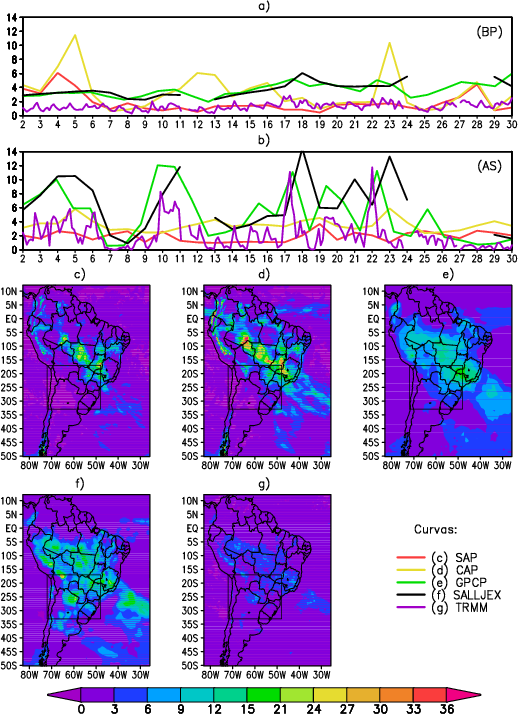
\includegraphics[height=15cm]{./figs/serie_precipitacao-FCT06h-new.png}
\caption{Seríes das previsões de 6 horas de precipitação. Em a) séries do modelo Eta (linhas vermelha – experimento SAP e amarela – experimento CAP), e GPCP (linha verde) para a região de avaliação destacada nas figuras ``c'', ``d'', ``e'', ``f'' e ``g''. Em b) Idem ``a'' para a AS. Em c), d) e e) os campos médios de precipitação para o experimentos SAP, CAP, GPCP, SALLJEX e TRMM. As unidades estão em $mm/dia$ nas séries e em $mm/m$\^{e}$s$ nos campos.}
\label{fig52}
\end{figure}

\break

\subsection{Avaliação da Temperatura e Umidade do Solo (SAP X CAP)}
\label{ss:avaltempumi}

Em relação à temperatura e umidade do solo, a versão do modelo Eta utilizada nos experimentos desta dissertação utiliza o modelo de superfície NOAH para o cálculo destas variáveis. Neste caso as condições iniciais de temperatura e umidade do solo são provenientes do modelo Global do CPTEC T126L28 e são atualizadas pelo modelo NOAH. A \autoref{fig50} mostra a série temporal da umidade do solo durante o período de assimilação (de 02 a 30 de Janeiro) do modelo Eta bem como os campos médios.

Nesta figura são mostradas as séries temporais da umidade do solo (entre 0 e 10 $cm$ - primeira camada) para os experimentos SAP e CAP, tanto para o domínio de integração do modelo (AS) quanto para a região de estudo (BP). Comparando-se os experimentos SAP e CAP, nota-se que o experimento CAP apresenta valores de umidade mais elevados do que o experimento SAP. Numericamente, a maior diferença entre as séries temporais é de $\sim$0,08 $kg/m^{2}$ para a região AS e de $\sim$0,02 $kg/m^{2}$ para a região BP.

Em relação à temperatura do solo (\autoref{fig51}), também observou-se que o experimento CAP apresentou valores diferentes em relação ao experimento SAP. Em média, estes valores não diferem muito (imagens ``c'' e ``d'' da \autoref{fig51}), sendo que menores valores podem ser encontrados na série do experimento CAP (linhas amarela e azul das imagens ``a'' e ``b''), tanto para a área de estudo (BP) quanto para o domínio de integração (AS).

\begin{figure}[!hbp]
\centering
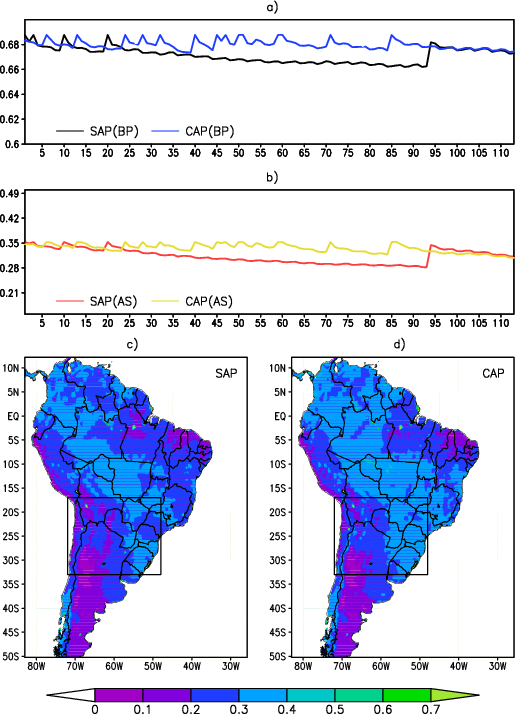
\includegraphics[height=15cm]{./figs/serie_umidade_solo-ANL-new.png}
\caption{a) e b) Série temporal da umidade do solo para a área de estudo (BP) e América do Sul (AS), respectivamente. c) e d) Campos médios da umidade do solo para os experimentos SAP e CAP, respectivamente. Linhas vermelha e preta representam o experimento SAP. Linhas amarela e azul, representam o experimento CAP. As unidades estão em $kg/m^{2}$.}
\label{fig50}
\end{figure}

\begin{figure}[!hbp]
\centering
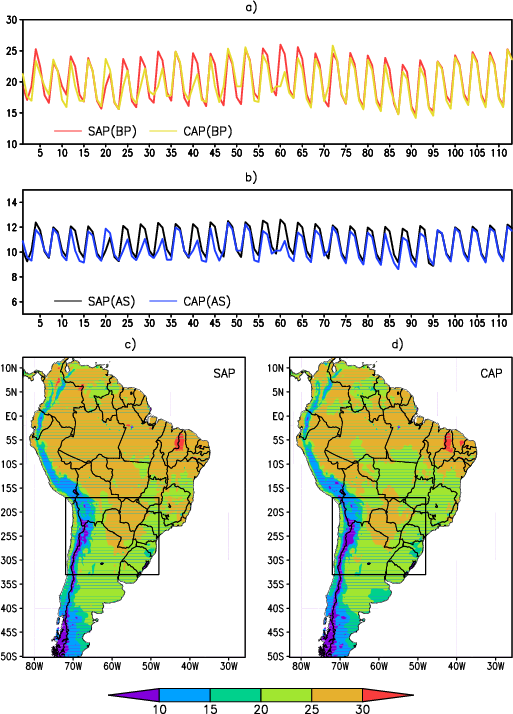
\includegraphics[height=15cm]{./figs/serie_temperatura_solo-ANL-new.png}
\caption{Idem \autoref{fig50}, para a Temperatura do Solo. As unidades estão em $ºC$.}
\label{fig51}
\end{figure}

\break

\subsection{Avaliação das Análises (Análises RPSAS X Reanálises)}
\label{ss:avalanl}

A \autoref{fig10} mostra os campos interpolados médios de Linha de Corrente para o nível de 850 $hPa$. Em a) tem-se o experimento SAP, em b) o experimento CAP, em c) a Reanálise do CPTEC e em d) a Reanálise 2 do NCEP/DOE (as demais figuras presentes nesta seção, seguem a mesma ordem de apresentação).

Comparando-se os dois experimentos (SAP e CAP), nota-se que em ambas as \-si\-mu\-la\-ções o padrão de escoamento é semelhante a partir do qual pode-se observar um escoamento de oeste sobre o Atlântico Subtropical e outro de leste sobre o norte da AS. Em relação à reanálises, a do CPTEC apresenta um padrão de circulação mais organizado apresentando também um giro anti-ciclônico bem definido sobre o Atlântico Subtropical dando suporte a esse escoamento de leste. Na reanálise do NCEP também observa-se esta confluência do escoamento de leste sobre o Atlântico Subtropical, e também o de oeste sobre o Norte da AS, porém um pouco menos intenso. Ambos os experimentos tenderam a simular uma circulação ao centro do continente, sendo esta mais bem caracterizada no experimento CAP. Este tipo de circulação ciclônica simulada pelo experimentos, pode ter sido causada pela tendência dos experimentos em apresentar maiores valores de temperatura à superfície (Temperatura à dois metros), o que pode ser observado na \autoref{fig11}. Neste caso os experimentos SAP e CAP apresentam valores mais elevados da temperatura em relação à reanálises. Além disso, as reanálises também divergem entre si no que se refere aos gradientes de temperatura que podem ser observados nas imagens da \autoref{fig11}. 

Este tipo de circulação apresentada pelos experimentos SAP e CAP é refletido em níveis mais altos, especialmente em 250 $hPa$ (\autoref{fig12}) em que o sentido do giro é contrário ao que ocorre em superfície. Este fenômeno pode ser observado nos quatro casos (nos dois experimentos e nas duas reanálises), porém com a diferença de que a reanálise do NCEP apresenta um vórtice anti-ciclônico bem definido, em comparação com os outros campos de circulação neste mesmo nível. Observa-se também que esta diferença é mais tênue em relação à reanálise do CPTEC, cujo campo de temperatua em altos níveis (250 $hPa$ – \autoref{fig13}) é mais semelhante ao da reanálise do NCEP.

Além disso, o padrão de circulação mostrado na \autoref{fig10}, mostra que existe um canal de vento que é mais bem caracterizado pelas reanálises do que pelos experimentos. Este canal de vento, mostrado na \autoref{fig15} (mais adiante) é característico do JBN. 

Em níveis médios (500 $hPa$ – \autoref{fig14}), os experimentos SAP e CAP também apresentam um padrão de circulação semelhante entre si divergindo pouco daquele apresentado pelas reanálises. Neste nível, a reanálise do NCEP apresenta um gradiente caracterizado por um escoamento de leste no nordeste da AS. Este padrão de escoamento foi simulado pelos experimentos e pela reanálise, no entanto, não foi bem caracterizado pelo experimento CAP e foi caracterizado de forma discreta pelo experimento SAP. Em comparação ao nível de 850 $hPa$, os experimentos parecem ser mais concordantes com as reanálises apresentando padrões de circulação mais semelhantes a essas. 

Nos campos de magnitude e direção do vento meridional em 850 $hPa$ e do vento zonal em 250 $hPa$ pode-se observer a presença dos jatos de baixos e altos níveis respectivamente.

A partir da descrição da média da componente meridional em 850 $hPa$ (\autoref{fig15}), é possível identificar o JBN que é caracterizado por ventos de norte/nordeste intensos em baixos níveis canalizados pela topografia dos Andes (bloqueio topográfico). Este tipo de jato fica bem caracterizado na média da reanálise do NCEP, havendo um pequeno sinal de sua atuação na reanálise do CPTEC. No entanto, não há sinal aparente de sua presença nas médias das simulações SAP e CAP. Este fato pode estar associado às caracaterísticas de circulação que foram encontradas nos campos de linha de corrente em 850 $hPa$ (\autoref{fig10}) em que pode-se perceber o contraste existente entre os experimentos e as reanálises. \citeonline{soaresmarengo04} apresentam um estudo de caso JBN à leste dos Andes sobre a AS, em Janeiro de 2003. Neste estudo, os autores identificaram um caso de JBN utilizando a reanálise 2 do NCEP/DOE. Os critérios de Bonner utilizados para a identificação do JBN são aqueles adaptados para AS. A partir destes critério, fica claro que os experimentos SAP e CAP não mostram evidências da atuação do JBN, principalmente porque a componente medional do vento em 850 $hPa$ é de sul com valores menores do 12 $ms^{1}$. Soares e Marengo também comparam simulações do modelo Eta de 40 $km$ (com condições de contorno do modelo global do CPTEC e com condições iniciais a análises do NCEP) e mostram que as previsões desse modelo tendem a subestimar os valores da magnitude da componente meridional do vento. Além disto, como trata-se das médias dos campos espaciais, possivelmente este fenômeno observado nas reanálises pode ter sido mascarada nos experimentos. Também, o fato de os experimentos SAP e CAP terem sido interpolados para a grade da reanálise do NCEP, pode penalizar o detalhamento associado à melhor resolução espacial dos experimentos realizados.

Entre outros aspectos que podem ser notados, pode-se citar que os experimentos e a reanálise do NCEP concordam sobre a intensidade do vento sobre a região norte do continente. Neste caso, a reanálise do CPTEC tende a superestimar a intensidade do vento em 850 $hPa$ em relação aos experimentos e reanálise do NCEP. 

Em 250 $hPa$, os campos da componente zonal do vento são mostrados na \autoref{fig16}. Neste nível, a presença dos Jatos de Altos Nível ao sul do continente é marcante e sua atuação é importante devido à influência que exercem na propagação de frentes atmosféricas e na formação de alguns sistemas convectivos. Os experimentos SAP e CAP, neste nível, apresentam características semelhantes de escoamento, tanto em relação à circulação quanto em relação à intensidade. O mesmo ocorre em relação às duas reanálises, sendo que a do NCEP fecha um vórtice (que pode ser visto no campo de linha de corrente da \autoref{fig12} - Alta da Bolívia). Este vórtice não é bem caracterizado pelos dois experimentos. 

Observa-se também que a magnitude desta componente do vento simulada pelos experimentos SAP e CAP é mais intensa neste nível, o que também pode ser notado no campo de linha de corrente em 250 $hPa$ (\autoref{fig12}) com gradientes zonais intensos, entre as latitudes de 30$ºS$ e 20$ºS$. No entanto, a posição e a intensidade dos Jatos é bem definida e coerente entre os quatros campos apresentados na \autoref{fig16}, com a componente zonal do vento apresentando valores máximos (acima de 24 $ms^{1}$) em relação às posições climatológicas de 35$ºS$ a 70$ºS$ para o Jato Polar (JP) – embora não mostrado e de 20$ºS$ a 30$ºS$ para o Jato Subtropical (JST). Estes valores podem ser encontrado em \citeonline{reiter69} e \citeonline{riehl69}. 

A comparação entre os experimentos e as reanálises do NCEP e do CPTEC para a temperatura do ar, mostra que para os três níveis avaliados (850, 500 e 250 $hPa$ – \autoref{fig20}, \autoref{fig21} e \autoref{fig13}, respectivamente) as temperaturas, em boa parte do continente (aproximadamente entre a faixa de latitudes de -20$ºS$ e 10$ºN$), tenderam a ser mais quentes ($\sim$2$ºC$ a mais do que as reanálises). Estas diferenças também podem ser notadas nas médias dos campos de Altura Geopotencial devido à relação existente (hipsométrica) entre temperatura e a espessura da camada acima.

\begin{figure}[!hbp]
\centering
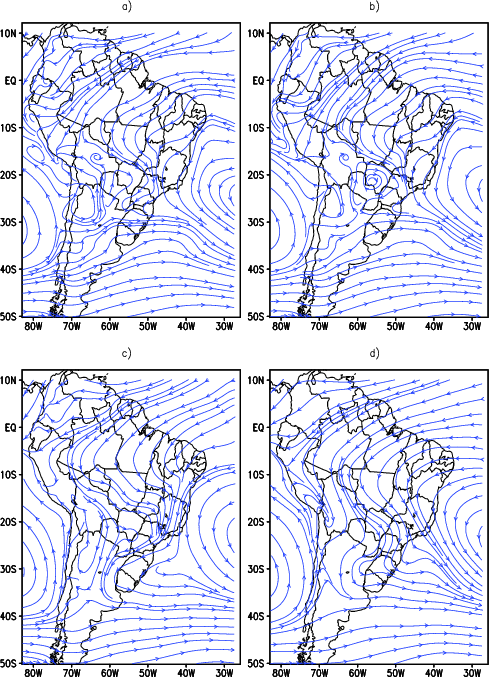
\includegraphics[height=15cm]{./figs/media_corrente_anl_850hPa.png}
\caption{Linha de Corrente para o nível de 850 $hPa$. a) experimento SAP, b) experimento CAP, c) Reanálise CPTEC, d) Reanálise 2 NCEP/DOE.}
\label{fig10}
\end{figure}

\begin{figure}[!hbp]
\centering
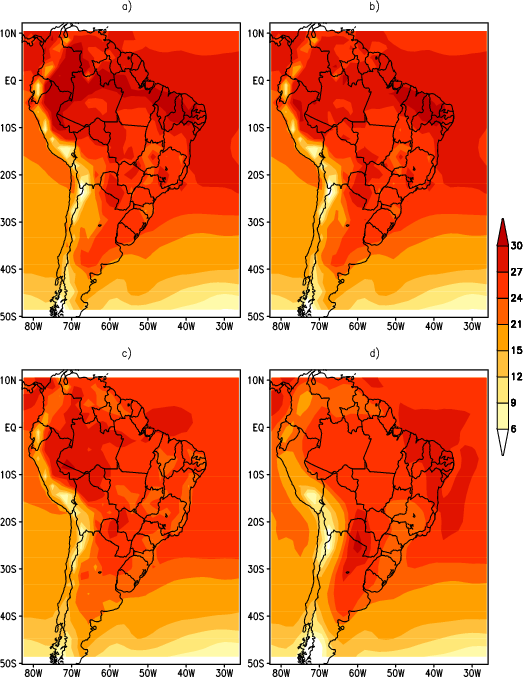
\includegraphics[height=15cm]{./figs/media_tp2m_anl.png}
\caption{Idem à \autoref{fig10}, para a Temperatura doa Ar à Superfície (T2M). As unidades estão em $ºC$.}
\label{fig11}
\end{figure}

\begin{figure}[!hbp]
\centering
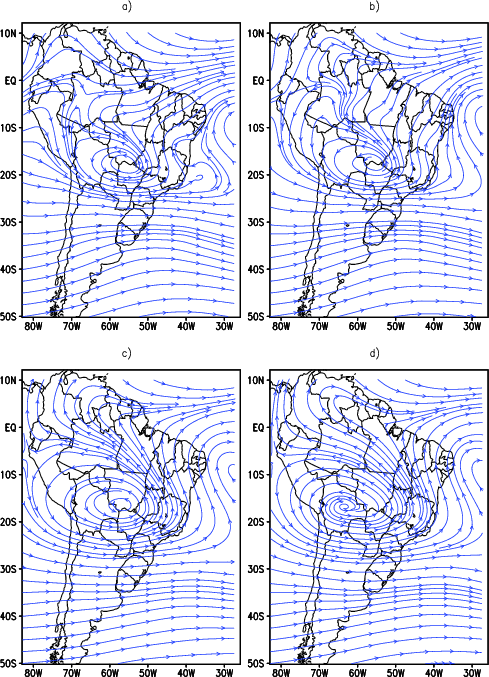
\includegraphics[height=15cm]{./figs/media_corrente_anl_250hPa.png}
\caption{Idem Figura 10, para o nível de 250 $hPa$.}
\label{fig12}
\end{figure}

\begin{figure}[!hbp]
\centering
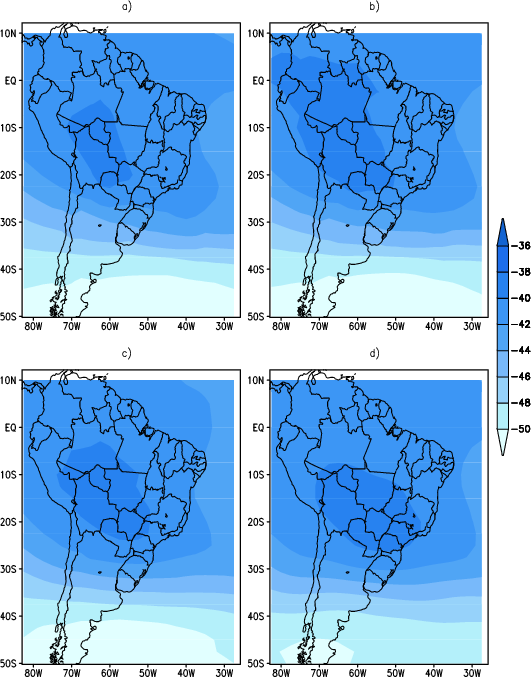
\includegraphics[height=15cm]{./figs/media_temp_anl_250hPa.png}
\caption{Temperatura do Ar para o nível de 250 $hPa$. As unidades estão em $ºC$.}
\label{fig13}
\end{figure}

\begin{figure}[!hbp]
\centering
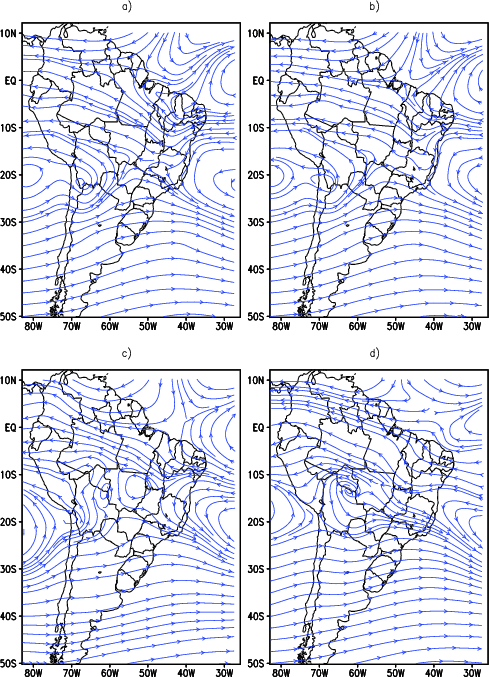
\includegraphics[height=15cm]{./figs/media_corrente_anl_500hPa.png}
\caption{Idem \autoref{fig10}, para o nível de 500 $hPa$.}
\label{fig14}
\end{figure}

\begin{figure}[!hbp]
\centering
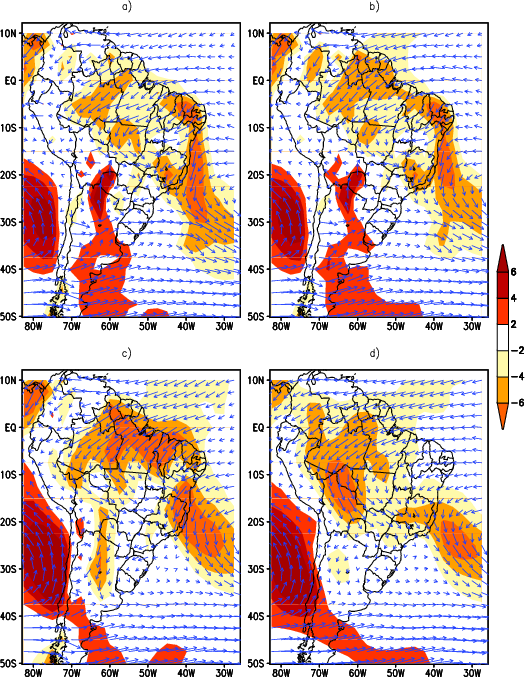
\includegraphics[height=15cm]{./figs/media_vento-meridional_anl_850hPa.png}
\caption{Componente Meridional do vento para o nível de 850 $hPa$. a) experimento SAP, b) experimento CAP, c) Reanálise CPTEC, d) Reanálise 2 NCEP/DOE. As unidades estão em $ms^{1}$.}
\label{fig15}
\end{figure}

\begin{figure}[!hbp]
\centering
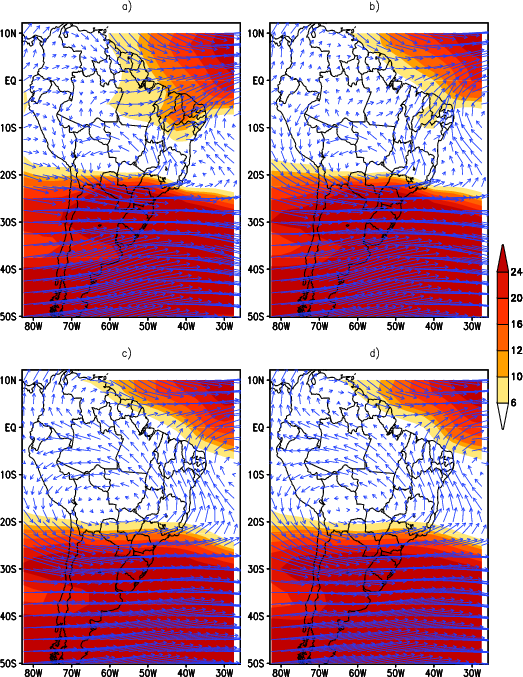
\includegraphics[height=15cm]{./figs/media_vento-zonal_anl_250hPa.png}
\caption{Componente Zonal do vento para o nível de 250 $hPa$. a) experimento SAP, b) experimento CAP, c) Reanálise CPTEC, d) Reanálise 2 NCEP/DOE. As unidades estão em $ms^{1}$.}
\label{fig16}
\end{figure}

\begin{figure}[!hbp]
\centering
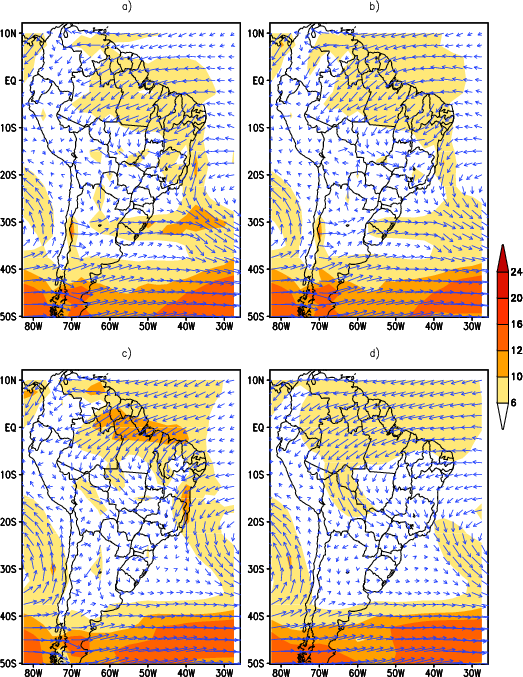
\includegraphics[height=15cm]{./figs/media_ventos_anl_850hPa.png}
\caption{Magnitude e direção do vento para o nível de 850 $hPa$. a) experimento SAP, b) experimento CAP, c) Reanálise CPTEC, d) Reanálise 2 NCEP/DOE. As unidades estão em $ms^{1}$.}
\label{fig17}
\end{figure}

\begin{figure}[!hbp]
\centering
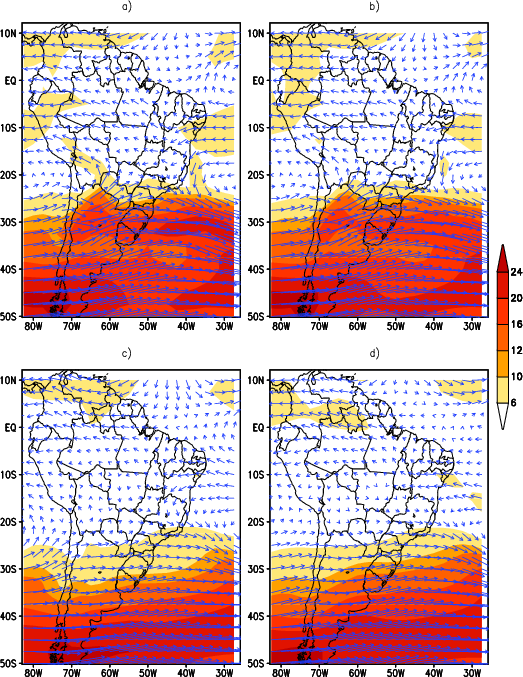
\includegraphics[height=15cm]{./figs/media_ventos_anl_500hPa.png}
\caption{Idem \autoref{fig17}, para o nível de 500 $hPa$.}
\label{fig18}
\end{figure}

\begin{figure}[!hbp]
\centering
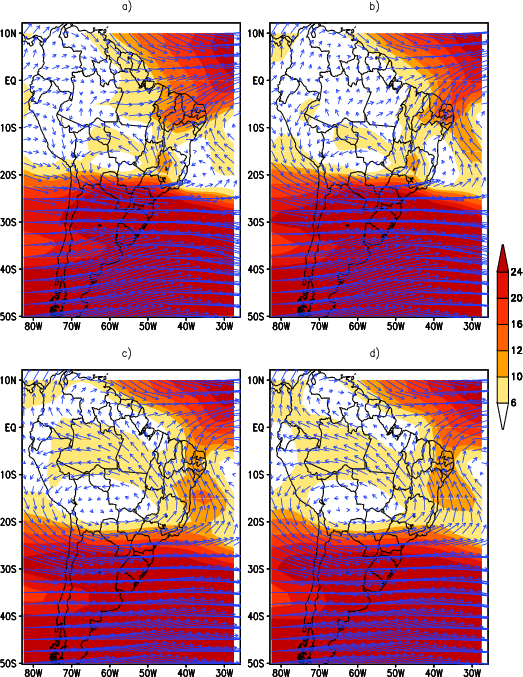
\includegraphics[height=15cm]{./figs/media_ventos_anl_250hPa.png}
\caption{Idem \autoref{fig17}, para o nível de 250 $hPa$.}
\label{fig19}
\end{figure}

\begin{figure}[!hbp]
\centering
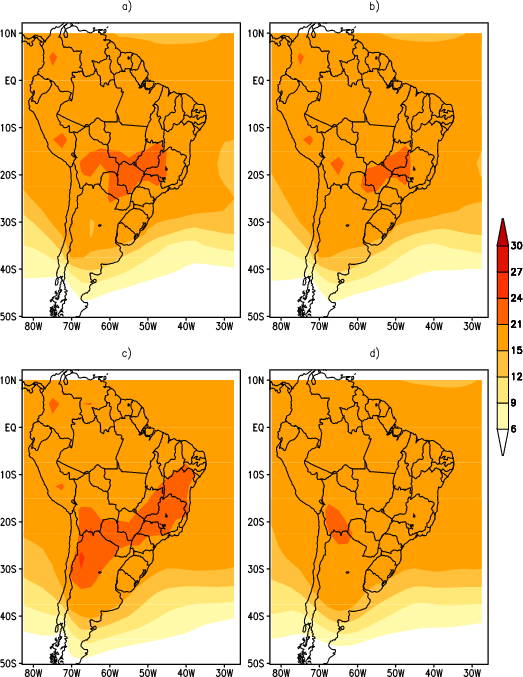
\includegraphics[height=15cm]{./figs/media_temp_anl_850hPa.png}
\caption{Idem \autoref{fig13}, para o nível de 850 $hPa$.}
\label{fig20}
\end{figure}

\begin{figure}[!hbp]
\centering
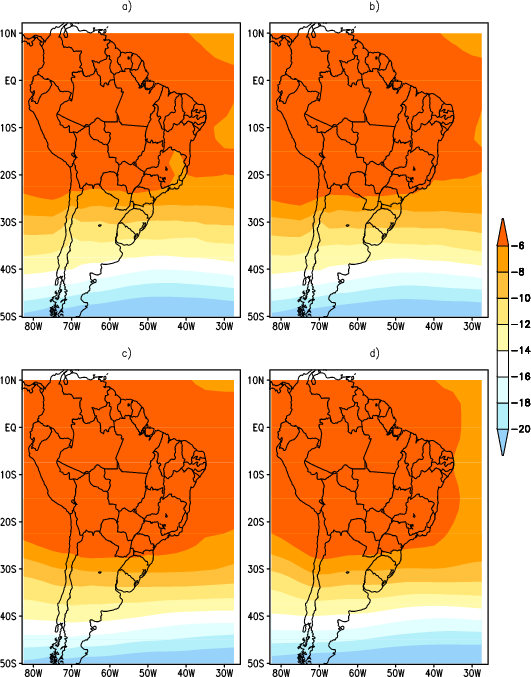
\includegraphics[height=15cm]{./figs/media_temp_anl_500hPa.png}
\caption{Idem \autoref{fig13}, para o nível de 500 $hPa$.}
\label{fig21}
\end{figure}

\subsection{Avaliação Espacial e das Séries Temporais das Análises (Análises RPSAS X Reanálise NCEP)}
\label{ss:avalesanl}

As figuras a seguir (\autoref{fig30a} até \autoref{fig34b}) mostram as séries temporais do Viés e do Erro Quadrático Médio das análises em relação à reanálise do NCEP, para os níveis de 850, 500 e 250 $hPa$ para as seguintes variáveis: Altura Geopotencial, Temperatura do Ar, Ventos Zonal e Meridional e Umidade Relativa, durante 02 e 30 de Janeiro de 2003.

Para a Altura Geopotencial (\autoref{fig30a} e \autoref{fig30b}), observa-se que os maiores valores de Viés e EQM estão no nível de 250 $hPa$ e sobre a região Sul do Brasil e Argentina. Comparativamente, os experimentos SAP e CAP tenderam a subestimar a altura geométrica do Geopotencial ($\sim$30 $mgp$), sendo que o experimento CAP apresentou um distribuição menor do erro do que o experimento SAP. Além disso, neste mesmo nível, o experimento CAP em algumas partes da região de avaliação, removeu o Viés negativo e em outras acabou por superestimar o valor do Viés. Consequentemente, a distribuição espacial do EQM para esta variável também é maior em altos níveis. Em 850 e 500 $hPa$, o valor do EQM para altura Geopotencial foi menor do que em 250 $hPa$, nível em que a distribuição espacial do EQM foi maior e acima de 20 $mgp$.

A temperatura, ao contrário do que foi encontrado para a Altura Geopotencial, apresentou maiores valores de Viés e EQM em superfície do que em médios e altos níveis (\autoref{fig31a} e \autoref{fig31b}). Em 850 $hPa$, a maior parte do Viés concentrou-se na região centro-oeste do Brasil apresentando valores positivos de Viés e em poucos pontos isolados valores negativos, como sobre o a região central da Argentina. Em 500 $hPa$, os valores de Viés foram menores havendo um deslocamento do Viés positivo da temperatura para a região oeste do continente, porém com valores menores. Sobre a região centro-oeste do continente, os valores negativos de Viés também foram minimizados. Já em 250 $hPa$, os erros foram bem menore se comparados aos valores de erro em superfície (850 $hPa$). Neste nível, porém, observa-se que uma pequena tendência de Viés positivo sobre o oceano Atlântico Subtropical. Sobre o Norte da Argentina, e comparativamente ao experimento SAP, o experimento CAP apresentou Viés muito próximo de zero. A distribuição espacial do EQM para a Temperatura Absoluta mostra claramente que os erros mais significativos entre os experimentos foram em baixos níveis.

As componentes Zonal e Meridional do vento (\autoref{fig32a} e \autoref{fig32b}, \autoref{fig33a} e \autoref{fig33a} respectivamente) avaliadas, mostram que maiores valores de Viés foram encontradas em 850 $hPa$ e 500 $hPa$, respectivamente. A distribuição espacial do Viés do vento meridional nestes dois níveis é semelhante entre ambos os experimentos, sendo que o experimento CAP tende a atenuar os valores máximos e mínimos do Viés. Em boa parte do continente, ambos os experimentos tendem a subestimar o valor da componente meridional do vento. Em algumas regiões (regiões central do continente e norte da Argentina), os experimentos apresentaram valores altos de Viés. Em 250 $hPa$, os valores de Viés apresentados pelos experimentos tendem a ser atenuados, embora o EQM apresentado por eles seja um pouco maior do que aqueles observados em 500 e 850 $hPa$. Já os valores de Viés e EQM calculados para os experimentos CAP e SAP para a componente zonal do vento, mostram que há uma tendência maior dos experimentos em superestimar os valores desta componente em altos níveis. Em 500 e 850 $hPa$, os valores de Viés tendem a ser menores ($\sim$5 $ms^{1}$), sendo que sobre o norte da Argentina e sul do Brasil, estes valores são levemente superestimados.

A avaliação do Viés e EQM da umidade relativa para os níveis de 850, 500 e 250 $hPa$ - \autoref{fig34a} e \autoref{fig34b}, mostra que em níveis médios (500 $hPa$)), os experimentos SAP e CAP foram menos tendenciosos em superestimar ou subestimar os valores relativos de umidade. Neste nível, foram encontrados menores valores de EQM. Em relação os níveis de 850 $hPa$ e 500 $hPa$, houve maior tendencia dos experimentos em subestimar a umidade do ar, sendo que novamente o experimento CAP atenuou os valores do Viés e do EQM.

A avaliação das séries temporais das análises do RPSAS em relação às análises do NCEP, mostram que, em geral, os maiores valores de erro (Viés) encontram-se no nível de 250 $hPa$, para o experimento SAP. O experimento CAP apresenta valores de Viés menores (se comparado com o experimento SAP), sugerindo que a assimilação de precipitação tende a retirar mais o Viés em superfície (850 $hPa$) e em médios níveis (500 $hPa$) do que em altos níveis. Esta avaliação é válida para as variáveis: ventos (componentes zonal e meridional), temperatura e umidade. A altura geopotencial, ao contrário do que se segue para as variáveis dinâmicas, apresenta maiores diferenças de Viés e EQM para o nível de 250 $hPa$. Isto pode ser explicado pelo fato de que os valores de Viés e EQM da variável Temperatura do Ar apresentarem maiores diferenças entre os experimentos em baixos e médios níveis, 850 e 250 $hPa$. A avaliação da distribuição espacial do Viés e do EQM reforçam este ponto de vista. 

\break

\begin{figure}[!h]
\centering
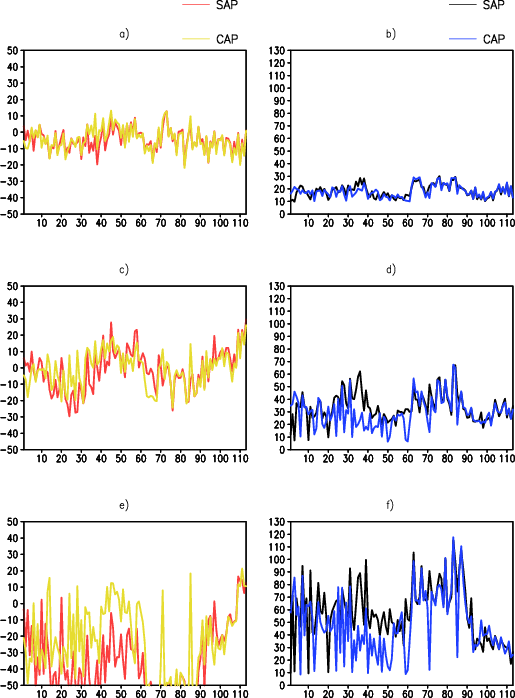
\includegraphics[height=15cm]{./figs/vies_eqm-zgeo.png}
\caption{Viés (coluna da esquerda) e Erro Quadrático Médio (coluna da direita) da Altura Geopotencial [$mgp$] para os níveis de 850 (primeira linha), 500 (segunda linha) e 250 $hPa$ (terceira linha). As linhas vermelha e preta representam o experimento SAP e as linhas amarela e azul, o experimento CAP. As unidades estão em $mgp$.}
\label{fig30a}
\end{figure}

\break

\begin{figure}[!h]
\centering
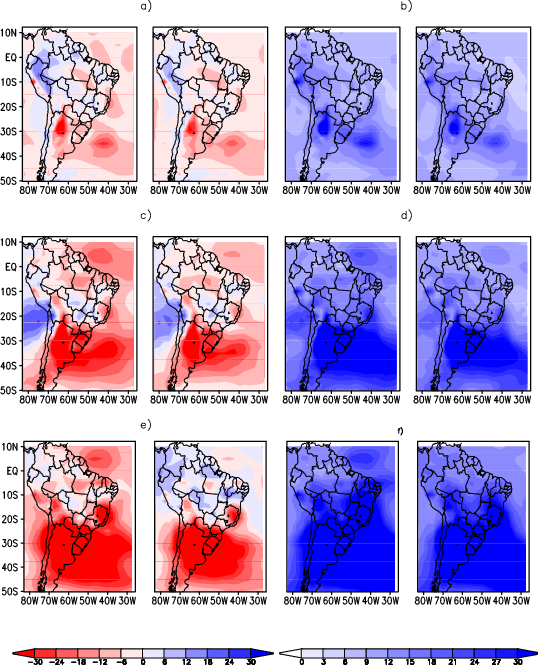
\includegraphics[height=15cm]{./figs/campo_vies_eqm-zgeo.png}
\caption{Viés e EQM espacial da Altura Geopotencial [$mgp$] para os níveis de a,b) 850 $hPa$; c,d) 500 $hPa$ e e,f) 250 $hPa$. As colunas 1 e 3 representam o Viés e o EQM para o experimento SAP, respectivamente. As colunas 2 e 4, representam o Viés e o EQM para o experimento CAP, respectivamente. As unidades estão em $mgp$.}
\label{fig30b}
\end{figure}

\break

\begin{figure}[!h]
\centering
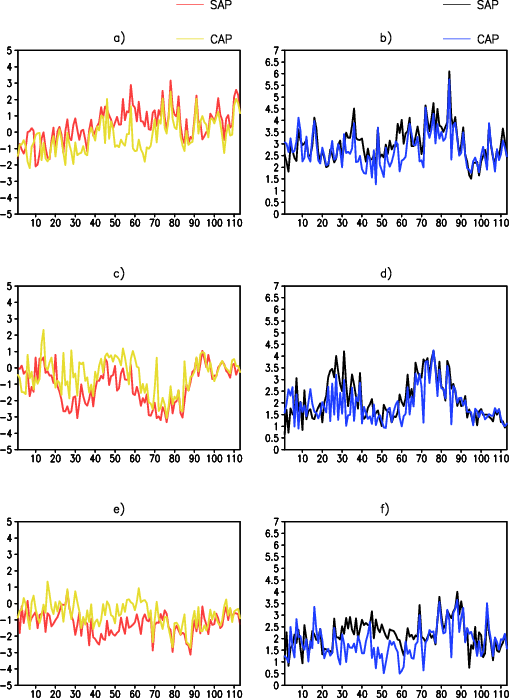
\includegraphics[height=15cm]{./figs/vies_eqm-temp.png}
\caption{Idem \autoref{fig30a}, para a Temperatura do Ar. As unidades estão em $ºC$.}
\label{fig31a}
\end{figure}

\break

\begin{figure}[!h]
\centering
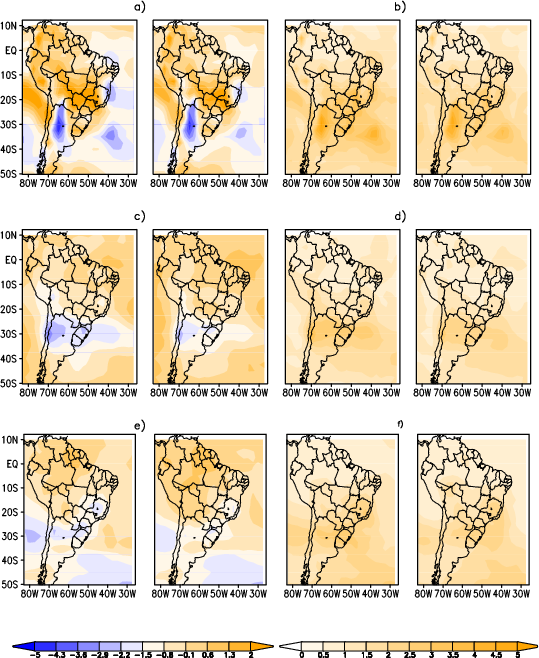
\includegraphics[height=15cm]{./figs/campo_vies_eqm-temp.png}
\caption{Idem \autoref{fig30b}, para a Temperatura do Ar. As unidades estão em $ºC$.}
\label{fig31b}
\end{figure}

\break

\begin{figure}[!h]
\centering
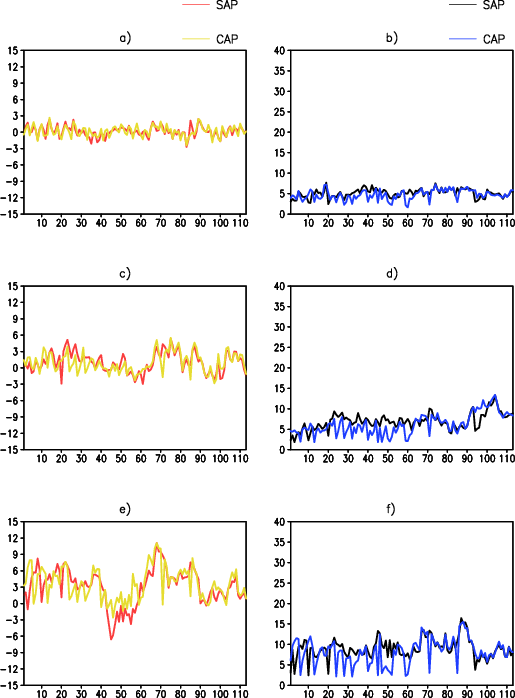
\includegraphics[height=15cm]{./figs/vies_eqm-uvel.png}
\caption{Idem \autoref{fig30a}, para o Vento Zonal. As unidades estão em $ms^{1}$.}
\label{fig32a}
\end{figure}

\break

\begin{figure}[!h]
\centering
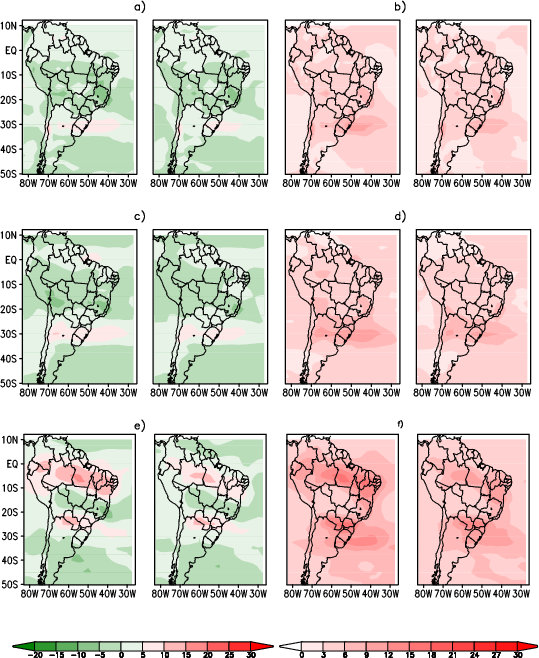
\includegraphics[height=15cm]{./figs/campo_vies_eqm-uvel.png}
\caption{Idem \autoref{fig30b}, para o Vento Zonal. As unidades estão em $ms^{1}$.}
\label{fig32b}
\end{figure}

\break

\begin{figure}[!h]
\centering
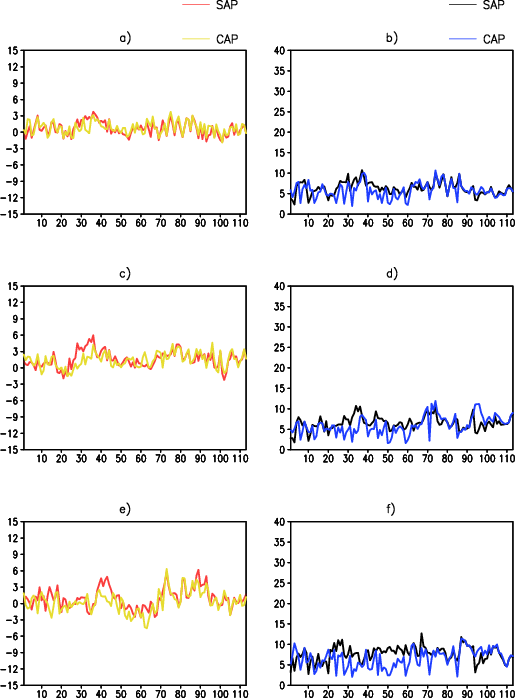
\includegraphics[height=15cm]{./figs/vies_eqm-vvel.png}
\caption{Idem \autoref{fig30a}, para Vento Meridional. As unidades estão em $ms^{1}$.}
\label{fig33a}
\end{figure}

\break

\begin{figure}[!h]
\centering
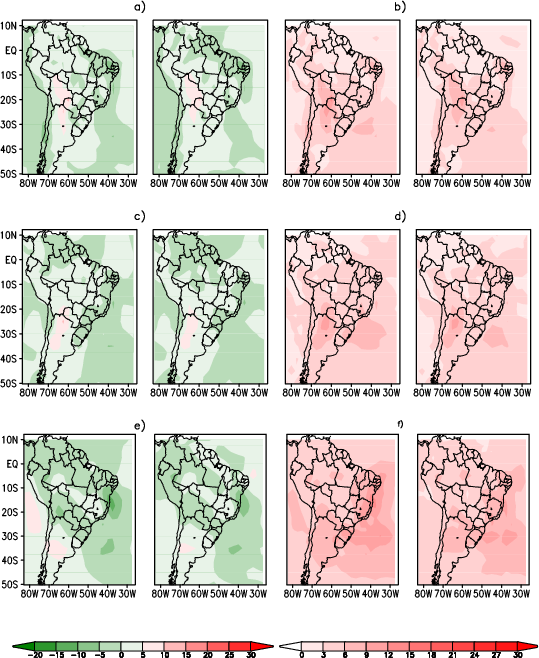
\includegraphics[height=15cm]{./figs/campo_vies_eqm-vvel.png}
\caption{Idem \autoref{fig30b}, para Vento Meridional. As unidades estão em $ms^{1}$.}
\label{fig33b}
\end{figure}

\break

\begin{figure}[!h]
\centering
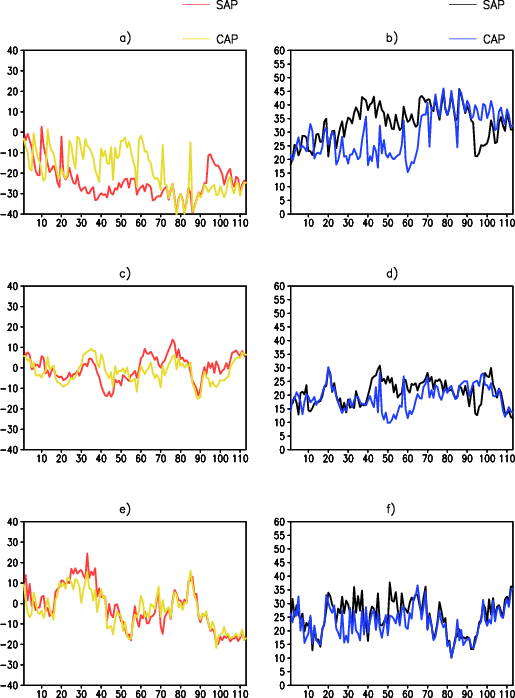
\includegraphics[height=15cm]{./figs/vies_eqm-umrl.png}
\caption{Idem \autoref{fig30a}, para a Umidade Relativa [\%].}
\label{fig34a}
\end{figure}

\break

\begin{figure}[!h]
\centering
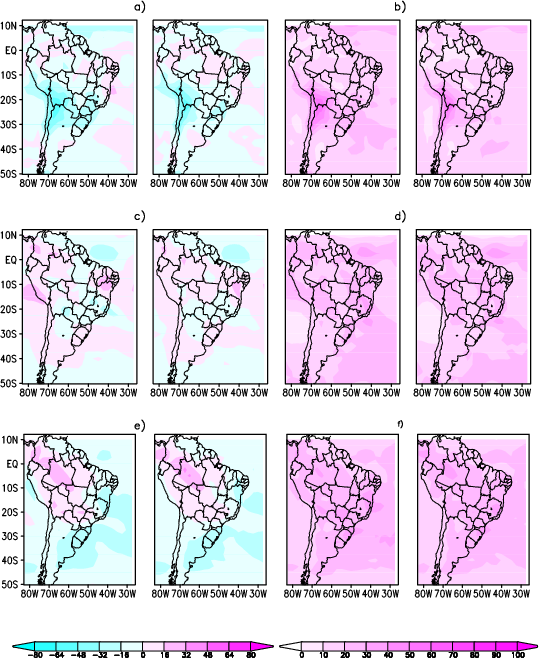
\includegraphics[height=15cm]{./figs/campo_vies_eqm-umrl.png}
\caption{Idem \autoref{fig30b}, para a Umidade Relativa [\%].}
\label{fig34b}
\end{figure}

\break

\section{Avaliação do \textit{Skill} do modelo Eta para as previsões de 6 a 24 horas}
\label{ss:avalskill}

Na \autoref{fig53} apresenta-se o Viés, EQM e CA da altura geopotencial para os horários das 00Z (coluna da esquerda) e 12Z (coluna da direita) para as previsões de 0 a 24 horas, no nível de 850 $hPa$. No geral nota-se que o experimento CAP apresenta resultados um pouco melhores no horário das 00Z durante 0 e 12 horas de previsão (figuras da coluna da esquerda) do que no horário das 12Z. No entanto, às 12Z (figuras da coluna direita) nota-se que em 12 horas de previsão o experimento CAP apresenta resultados um pouco melhores. Isso pode ser devido ao fato de que às 12Z a quantidade de observações sinótica é um pouco mais abundante do que às 00Z. Além disso, este resultado indica que o modelo se ajustou aos dados de precipitação assimilados, se comparado com o viés presente em 6 horas de previsão e em comparação com o experimento de controle SAP, que neste mesmo horário apresenta viés quase igual a zero. Em relação ao desempenho, embora os valores de CA se apresentem aquém em relação ao que se conhece do modelo operacional Eta do CPTEC - mas considerando-se a metodologia apresentada, nota-se que o desempenho do experimento CAP, na média, foi melhor no horário das 12Z do que às 00Z. Novamente, isto pode ser devido ao fato de haver uma maior abundância de dados sinóticos assimilados na análise das 12Z, o que levou o modelo a se ajustar mais rapidamente aos dados de precipitação assimilados pelo Eta.

\break

\begin{figure}[!hbp]
\centering
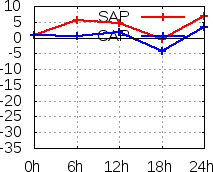
\includegraphics[height=4.7cm]{./figs/VIES850zgeo0Z.png}\vspace{1.0cm}\hspace{1.0cm}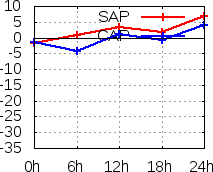
\includegraphics[height=4.7cm]{./figs/VIES850zgeo12Z.png}
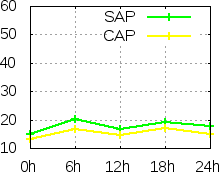
\includegraphics[height=4.7cm]{./figs/EQM850zgeo0Z.png}\vspace{1.0cm}\hspace{1.0cm}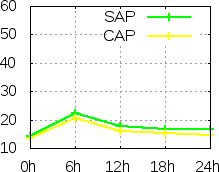
\includegraphics[height=4.7cm]{./figs/EQM850zgeo12Z.png}
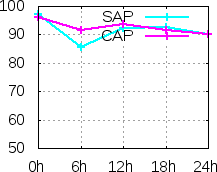
\includegraphics[height=4.7cm]{./figs/CA850zgeo0Z.png}\hspace{1.0cm}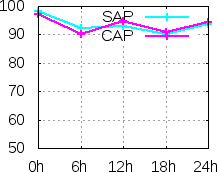
\includegraphics[height=4.7cm]{./figs/CA850zgeo12Z.png}
\caption{Viés, EQM e CA para a variável altura geopotencial em 850 $hPa$. A coluna da esquerda mostra os valores das medidas para o horário das 00Z. A coluna da esquerda mostra os valores das medidas para o horário das 12Z.}
\label{fig53}
\end{figure}

A próxima figura (\autoref{fig54}) mostra os valores dos índices estatísticos para a altura geopotencial no nível de 500 $hPa$.

\begin{figure}[!hbp]
\centering
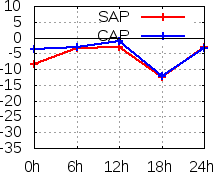
\includegraphics[height=4.7cm]{./figs/VIES500zgeo0Z.png}\vspace{1.0cm}\hspace{1.0cm}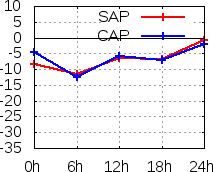
\includegraphics[height=4.7cm]{./figs/VIES500zgeo12Z.png}
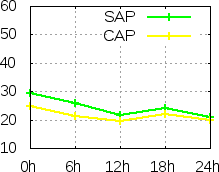
\includegraphics[height=4.7cm]{./figs/EQM500zgeo0Z.png}\vspace{1.0cm}\hspace{1.0cm}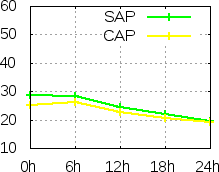
\includegraphics[height=4.7cm]{./figs/EQM500zgeo12Z.png}
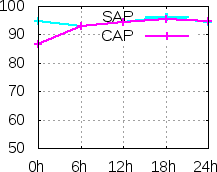
\includegraphics[height=4.7cm]{./figs/CA500zgeo0Z.png}\hspace{1.0cm}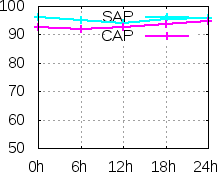
\includegraphics[height=4.7cm]{./figs/CA500zgeo12Z.png}
\caption{Viés, EQM e CA para a variável altura geopotencial em 500 $hPa$. A coluna da esquerda mostra os valores das medidas para o horário das 00Z. A coluna da esquerda mostra os valores das medidas para o horário das 12Z.}
\label{fig54}
\end{figure}

\break

Analisando-se o a altura geopotencial no nível de 500 $hPa$, observa-se que os valores de viés para ambos os experimentos tendem a ser negativos durante todo o período de previsão (de 0 a 24 horas). Isto significa que os experimentos SAP e CAP subestimaram o valor do geopotencial em níveis médios fazendo com que os valores do EQM aumentassem de 10 $mgp$ para valores entre 20 e 30 $mgp$. Observa-se um distanciamento sensível dos valores apresentados pelos experimentos em relação à Reanálise em 18 horas de previsão, no horário das 00Z. Este diferença é refletida nos valores do EQM, mas não afeta o desempenho geral do experimento CAP que, durante as 24 horas de previsão, apresentou pequena diferença em relação ao experimento de controle SAP. No horário das 12Z, o experimento CAP mostra-se melhor durante as 24 horas de previsão. Aparentemente, a quantidade de dados sinóticos assimilados, influencia a composição do campo de geopotencial pelo modelo, sendo (a \textit{priori}) um indicativo da necessidade de mais dados de observação para a melhoria da condição inicial do modelo, tal como foi verificado por \citeonline{andreolietal08}.

Nos dois experimentos avaliados (SAP e CAP), utilizou-se como primeira condição inicial a análise do NCEP. Posteriormente, após o primeiro ciclo de previsões, o próprio sistema Eta+RPSAS gerou a análise utilizada nos ciclos subsequentes. Na avaliação destes resultados utilizou-se também um produto puramente de modelagem que é a Reanálise. Comparar dados de previsão, que embora sejam corrigidos por observações sinóticas, mas que tendem a se distanciar da verdade com o passar do tempo, pode ser tendencioso no sentido de se onerar a qualidade das previsões dos experimentos e dar mais peso à modelagem. Isso pode acontecer porque a Reanálise se utiliza de dados modelados para reproduzir o estado passado da atmosfera, quase que de forma inversa ao que é feito com a previsão de tempo, onde se utiliza dados observados para se representar o estado presente ou futuro da atmosfera. Com isso, o produto que se obtém da Reanálise possui uma qualidade muito grande porque nela está contida a maior quantidade possível de dados observados que, em comparação à realidade dos experimentos, pode não ser verdade.

A seguir (\autoref{fig55}) são apresentados os resultados do Viés, do EQM e da CA para a temperatura do ar.

\break

\begin{figure}[!hbp]
\centering
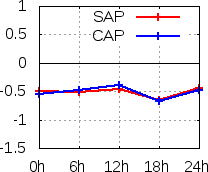
\includegraphics[height=4.7cm]{./figs/VIES850temp0Z.png}\vspace{1.0cm}\hspace{1.0cm}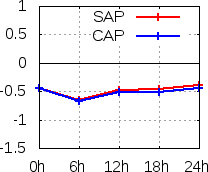
\includegraphics[height=4.7cm]{./figs/VIES850temp12Z.png}
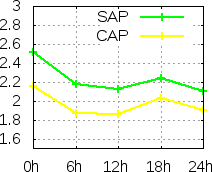
\includegraphics[height=4.7cm]{./figs/EQM850temp0Z.png}\vspace{1.0cm}\hspace{1.0cm}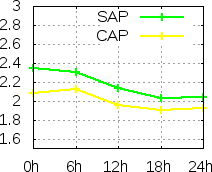
\includegraphics[height=4.7cm]{./figs/EQM850temp12Z.png}
\includegraphics[height=4.7cm]{./figs/CA850temp0Z.png}\hspace{1.0cm}\includegraphics[height=4.7cm]{./figs/CA850temp12Z.png}
\caption{Viés, EQM e CA para a variável temperatura do ar em 850 $hPa$. A coluna da esquerda mostra os valores das medidas para o horário das 00Z. A coluna da esquerda mostra os valores das medidas para o horário das 12Z.}
\label{fig55}
\end{figure}

A avaliação dos índices estatísticos considerados para a variável temperatura em 850 $hPa$, sugere que, em geral, os experimentos CAP e SAP não divergem muito em relação à estimativa dos campos produzidos para esta variável. Os valores de viés apresentados por ambos os experimentos são semelhantes. As diferenças mais significativas, no entanto, surgem nos valores de EQM e CA. Em relação ao erro quadrático médio, o experimento CAP apresentou valores menores de erro em ambos os horários sendo que a maior diferença entre os dois experimentos para este índice, se ocorreu no horário das 00Z. Às 12Z este diferença tende a ser menor (possivelmente devido à maior quantidade de dados disponíveis para assimilação). No entanto, o índice CA mostra que apenas durante as 6 primeiras horas de previsão das 12Z é que o experimento CAP obteve melhor reultado em relação ao experimento SAP. Outro fator que pode ser associado a este resultado é a dependência de que a precipitação tem dos processos de escala de subgrade, seja na liberação de calor latente ou na modulação do perfil vertical de umidade, o qual a temperatura está associada.

A assimilação de precipitação pelo modelo Eta é um processo de \textit{nudging}, onde as variáveis prognósticas do modelo são inicializadas de acordo com as alterações nos perfis verticais de temperatura e umidade. Estes perfis são alterados quando se compara a precipitação produzida pelo modelo em relação à precipitação observada (conforme explicado na \autoref{tab03}). A temperatura é uma das variáveis que são diretamente influenciadas pelas alterações nos perfis de calor e umidade, devido à sua condição de referência no esquema de convecção. 

Os gráficos da \autoref{fig56} e \autoref{fig57}, mostram os valores dos índices de Viés, EQM e CA para a temperatura do ar nos níveis de 500 e 250 $hPa$. Em médios e altos níveis, observa-se que o viés da temperatura tende a apresentar um comportamento semelhante ao apresentado em baixos níveis, reforçando a idéia de que a temperatura é sensível às alteração de calor e umidade. Em geral, observa-se que o experimento CAP subestima menos os valores de temperatura do que o experimento SAP. Neste caso, nota-se que em níveis médios, o experimento CAP consegue reduzir bem o valor do viés (chegando a aproximadamente zero) em 6 horas de previsão, às 00Z. Em altos níveis isto também ocorre no mesmo horário, porém em 12 horas de previsão. Em relação aos valores de CA, observa-se que ambos os experimentos possuem um comportamento semelhante: em 850 $hPa$, os valores tendem a ser menores do que em 500 $Pa$ e menores também do que em 250 $hPa$. Observa-se também que, em 500 e 250 $hPa$, o experimento SAP tendeu a ser um pouco melhor do que o experimento CAP, apresentando valores de CA um pouco mais elevados.

\begin{figure}[!hbp]
\centering
\includegraphics[height=4.7cm]{./figs/VIES500temp0Z.png}\vspace{1.0cm}\hspace{1.0cm}\includegraphics[height=4.7cm]{./figs/VIES500temp12Z.png}
\includegraphics[height=4.7cm]{./figs/EQM500temp0Z.png}\vspace{1.0cm}\hspace{1.0cm}\includegraphics[height=4.7cm]{./figs/EQM500temp12Z.png}
\includegraphics[height=4.7cm]{./figs/CA500temp0Z.png}\hspace{1.0cm}\includegraphics[height=4.7cm]{./figs/CA500temp12Z.png}
\caption{Viés, EQM e CA para a variável temperatura do ar em 500 $hPa$. A coluna da esquerda mostra os valores das medidas para o horário das 00Z. A coluna da esquerda mostra os valores das medidas para o horário das 12Z.}
\label{fig56}
\end{figure}

\begin{figure}[!hbp]
\centering
\includegraphics[height=4.7cm]{./figs/VIES250temp0Z.png}\vspace{1.0cm}\hspace{1.0cm}\includegraphics[height=4.7cm]{./figs/VIES250temp12Z.png}
\includegraphics[height=4.7cm]{./figs/EQM250temp0Z.png}\vspace{1.0cm}\hspace{1.0cm}\includegraphics[height=4.7cm]{./figs/EQM250temp12Z.png}
\includegraphics[height=4.7cm]{./figs/CA250temp0Z.png}\hspace{1.0cm}\includegraphics[height=4.7cm]{./figs/CA250temp12Z.png}
\caption{Viés, EQM e CA para a variável temperatura do ar em 250 $hPa$. A coluna da esquerda mostra os valores das medidas para o horário das 00Z. A coluna da esquerda mostra os valores das medidas para o horário das 12Z.}
\label{fig57}
\end{figure}

%% CAPITULO 4
\hypertarget{estilo:capitulo}{}
\chapter{ESTUDO DE CASO DE COMPLEXO CONVECTIVO DE MESOESCALA}
\label{ss:cap4}

Durante o período do projeto SALLJEX, foram identificados em torno de 100 SCMs entre as bacias Amazônica e do Prata, no Altiplano Sul-americano. No mês de Janeiro de 2003, ocorreram dois casos de CCMs, o primeiro no dia 18 de Janeiro e o segundo no dia 23 de Janeiro. Autores como \citeonline{zipseretal04} estudaram estes eventos e outros estudos numéricos foram realizados com o objetivo de se verificar se os modelos de PNT eram capazes de simular as principais características dos CCMs. \citeonline{paegleetal04} comparam vários modelos regionais, dentre eles versões diferentes dos modelos RAMS, MM5 e Eta (incluindo o modelo regional operacional, na época, do CPTEC - Eta 40 $km$). Os autores mostram que existe uma grande variação entre as previsões dos diferentes modelos e apontam as possíveis causas como sendo condições iniciais e de contorno não muito realistas, dados de baixa qualidade, dinâmica e parametrizações físicas inadequadas para a simulação desse tipo de fenômenos meteorológicos em regiões específicas do globo. Neste mesmo caso, os autores mostram também, como exemplo, o caso do CCM ocorrido no dia 18 de Janeiro em que os modelos regionais não foram capazes de simular as principais características do CCM. Em altas resoluções (e.g., 20 $km$), os modelos regionais são capazes de prever grandes acumulados de precipitação, mas, no entanto, não refletem bem as características associada aos SCMs. \citeonline{paegleetal04} ainda apontam para o fato de que a inicialização e a validação dos modelos podem beneficiar a análises geradas pelos modelos de previsão.

Para este estudo de caso, foi escolhido o CCM ocorrido no dia 23 de janeiro de 2003. Em \citeonline{rozantecavalcanti06} são feitas simulações sobre o CCM do dia 18 de Janeiro de 2003 e outros experimentos numéricos com o modelo Eta durante o período da campanha do SALLJEX. 

Na \autoref{fig61} são mostradas as imagens do canal 4 (infravermelho) do satélite \textit{Geostationary Satellite Server} (GOES) 8. Nestas imagens, pode-se observar um CCM que começou a se formar no dia 22 de janeiro de 2003 às 18Z, tendo seu ciclo de vida com duração total de um dia, culminando ao dia 23 de janeiro de 2003 às 12Z. Na \autoref{fig62}, é mostrada a precipitação diária observada do SALLJEX, acumulada às 12Z.

\begin{figure}
\centering
a)\includegraphics[height=4.3cm]{./figs/sat01.png}\hspace{0.2cm}b)\includegraphics[height=4.3cm]{./figs/sat02.png}\hspace{0.2cm}
c)\includegraphics[height=4.3cm]{./figs/sat03.png}\hspace{0.2cm}d)\includegraphics[height=4.3cm]{./figs/sat04.png}
\\[0.15cm]
e)\includegraphics[height=4.3cm]{./figs/sat05.png}\hspace{0.2cm}f)\includegraphics[height=4.3cm]{./figs/sat06.png}\hspace{0.2cm}
g)\includegraphics[height=4.3cm]{./figs/sat07.png}\hspace{0.2cm}h)\includegraphics[height=4.3cm]{./figs/sat08.png}
\caption{Imagens do Satélite GOES 8 no canal 4 (infravermelho). Evolução de um Complexo Convectivo de Mesoescala. Nas figuras: a) 20030122$\_$18Z; b) 20030122$\_$21Z; c) 20030123$\_$00Z; d) 20030123$\_$03Z; e) 20030123$\_$06Z; f) 20030123$\_$09Z; g) 20030123$\_$12Z; h) 20030123$\_$15Z.}
\label{fig61}
\end{figure}

\begin{figure}
\centering
\includegraphics[height=15cm]{./figs/prec_salljex1.png}
\caption{Precipitação observada diária SALLJEX, acumulados das 12Z. Nas figuras: a) 20030122$\_$12Z; b) 20030123$\_$12Z; c) 20030124$\_$12Z.}
\label{fig62}
\end{figure}

\break

Com as simulações dos experimentos SAP e CAP, buscou-se observar se o modelo de previsão Eta e o sistema de assimilação de dados RPSAS foram capazes de simular esse complexo convectivo, através da simulação dos seguintes parâmetros: ciclo de vida (duração), intensidade, posicionamento e precipitação associada.

Diante das configurações ajustadas para o modelo de previsão Eta (com e sem a assimilação de precipitação, com filtro digital e no modo hidrostático), e comparando-se o resultado dos experimentos com os dados do SALLJEX e do TRMM, pode-se notar que sem a assimilação de precipitação (experimento SAP), o modelo não foi capaz de reproduzir o evento de precipitação ocasionado pelo CCM. Apenas com a assimilação de precipitação (experimento CAP), o modelo foi capaz de reproduzir a precipitação ocasionada pelo CCM.

Para efeito de comparação, vale lembrar que durante o experimento de campo do SALLJEX, foram instalados vários pluviógrafos adicionais na região de estudo o que favoreceu uma descrição muito mais minuciosa dos acumulados de precipitação. A precipitação do TRMM3B42, embora possua uma resolução temporal mais refinada (3 horas), mostra que em seus acumulados uma distribuição de precipitação mais discreta do que a do SALLJEX, principalmente às 06Z do dia 23 de Janeiro de 2003, quando o CCM atinge seu estágio maduro. O campo de precipitação produzido pelo modelo Eta, com o experimento CAP, apresenta também taxas de precipitação inferiores àquelas observadas no SALLJEX, embora sua distribuição espacial seja concordante com o que foi encontrado na observação.

Observando-se as imagens do canal infravermelho do GOES 8, nota-se que o CCM começou a se formar às 18Z do dia 22 de Janeiro e atinge o seu estágio maduro (o máximo de precipitação) às 06Z do dia 23, quando observa-se os critérios de forma tamanho e tempo de duração definidos por \citeauthoronline{maddox80} para a caracterização do CCM.

As imagens da \autoref{fig63} mostram a precipitação estimada do TRMM correspondentes às imagens de satélite do GOES 8.

\begin{figure}[!hpb]
\centering
\includegraphics[height=15cm]{./figs/prec_trmm3b42.png}
\caption{Precipitação Estimada TRMM3B42. Evolução de um CCM. Nas figuras: a) 20030123$\_$00Z; b) 20030123$\_$03Z; c) 20030123$\_$06Z; d) 20030123$\_$09Z; e) 20030123$\_$12Z; f) 20030123$\_$15Z; g) 20030123$\_$18Z; h) 20030123$\_$21Z.}
\label{fig63}
\end{figure}

\break

Os campos de precipitação produzidos pelo modelo Eta com os experimentos SAP e CAP, mostram diferenças significativas durante as previsões de 6, 12, 18 e 24 horas. A assimilação dos dados de precipitação fez com que o modelo Eta reproduzisse de forma relativamente satisfatória o campo de precipitação apresentado na imagem ``c'' da \autoref{fig63}. No entanto, levando-se em consideração os esquemas físicos do modelo,  a melhor discretização dos tipos de solo do modelo de superfície NOAH e o esquema de convecção BMJ, nota-se também que as simulações do experimento CAP tendem a superestimar e a espalhar um pouco mais a precipitação nos horários subsequentes à 06Z do dia 23 de Janeiro (\autoref{fig64}).

\begin{figure}[!hpb]
\centering
\includegraphics[height=15cm]{./figs/prec_eta1.png}
\caption{Precipitação Prevista pelo sistema Eta+RPSAS a partir do dia 23/01/2003. Nas figuras: (primeira coluna) previsões de a) 6h; b) 12h; c) 18h e d) 24h para o experimento SAP, (segunda coluna) previsões e) 6h; f) 12h; g) 18h e h) 24h para o experimento CAP.}
\label{fig64}
\end{figure}

\break


Para efeito de se verificar a quantidade de umidade transportada pelo JBN a disponível para a atividade convectiva, a \autoref{fig66} mostra a seção vertical do fluxo de umidade para a latitude de 22$ºS$. Nesta figura são mostrados os resultados encontrados para os experimentos SAP (primeira linha) e CAP (segunda linha). Nesta figura nota-se que o fluxo de umidade apresentado pelo experimento CAP às 06Z do dia 23 apresenta valores elevados (da ordem de 100 $g/kg$ $m/s$).

\begin{figure}[!h]
\centering
\includegraphics[height=10.5cm]{./figs/sec_vert_flux_umi.png}
\caption{Seção vertical do fluxo de umidade ($qv$) ao longo da latitude de 22$ºS$, às 18Z do dia 22 (coluna da esquerda - letras ``a'' e ``d''), às 00Z do dia 23 (coluna do meio - ``b'' e ``e'') e às 06Z do dia 23 de Janeiro (coluna da direita - letras ``c'' e ``f''). Os contornos estão em $g/kg$ $m/s$.}
\label{fig66}
\end{figure}

A \autoref{fig67} mostra os campos de velocidade vertical (Omega) em 700 $hPa$ para os experimentos SAP e CAP e a precipitação do SALLJEX. Comparando-se os dois experimentos, nota-se que o experimento CAP foi capaz de detalhar melhor o desenvolvimento vertical das nuvens convectivas associadas ao CCM. Os sombreados em ciano representam valores de -0.2 $Pa/s$. Em \citeonline{herdiesetal07} estes valores são de -0.5 $Pa/s$.
 
\begin{figure}[!ht]
\centering
\includegraphics[height=8.5cm]{./figs/omega.png}
\caption{Velocidade vertical em 700 $hPa$ para os experimentos a) SAP e b) CAP. Em ambos os casos são mostradas as previsões de 6 horas. Em c) precipitação observada do SALLJEX. Os sombreados em ciano apresentam valores iguais a -0.2 $Pa/s$.}
\label{fig67}
\end{figure}

%% CAPITULO 5
\hypertarget{estilo:capitulo}{}
\chapter{CONCLUSÕES E SUGESTÕES}
\label{ss:cap5}

A inclusão da precipitação no ciclo do sistema Eta+RPSAS, tem como principal objetivo reduzir o tempo de \textit{spin up} do modelo Eta e melhorar as condições iniciais de temperatura e umidade do solo, e consequentemente aprimorar a representação dos sistemas convectivos, especialmente aqueles relacionados à convecção profunda, tais como os SCMs. Nesta dissertação de mestrado foi investigado o impacto causado pela inclusão dos dados estimados de precipitação do TRMM no ciclo de análises e previsões do sistema Eta+RPSAS, através da avaliação estatística do \textit{skill} do modelo Eta e de um estudo de caso de CCM.

Em relação às análises produzidas pelo sistema RPSAS, em comparação com as reanálises do NCEP e do CPTEC, o Viés e o Erro Quadrático Médio, em geral, apresentaram valores menores para o experimento CAP (com assimilação de precipitação) e valores maiores para o experimento SAP (sem assimilação de precipitação). Nesta avaliação, os melhores resultados foram encontrados para
a Altura Geopotencial em 500 hPa e em 250 hPa, a Temperatura do Ar e Ventos Zonal e Meridional em 250 hPa e Umidade Relativa em 850 hPa.

A partir da avaliação do \textit{skill} do modelo (cálculo do Viés, Erro Quadrático Médio e Correlação de Anomalia - calculados em relação às reanálises do NCEP), pôde-se notar que com a assimilação de precipitação houve uma pequena redução do Viés e do Erro Quadrático Médio, significando uma redução sensível do erro sistemático do modelo Eta no prognóstico das variáveis verificadas (Altura Geopotencial, Ventos Zonal e Meridional e Temperatura). No entanto, não foram encontradas grandes melhorias em relação à acurácia (Correlação de Anomalia) da previsão do modelo Eta para a previsão de 24 horas. Parte deste resultado pode ser devido à metodologia (dados e método de avaliação) adotada para o trabalho. Possivelmente, a utilização das taxas instantâneas de precipitação do TRMM 3B41 sejam mais apropriadas para inclusão no ciclo do sistema Eta+RPSAS, devido à sua amostragem espaço-temporal. Sistemas de mesoescala tendem a deslocar-se e intensificar-se rapidamente em um curto período tempo (tipicamente 1 hora). Portanto, em 3 horas um sistema desse gênero pode evoluir rapidamente em seu ciclo de vida. A idéia principal da inclusão de precipitação é corrigir instantaneamente as condições iniciais de solo (e consequentemente atmosféricas) e que modulam o desenvolvimento convectivo desses sistemas melhorando o diagnóstico da precipitação pelo sistema de análise/previsão.

Durante os meses de Novembro de 2002 a Fevereiro de 2003, foi realizado um dos maiores experimentos de campo - SALLJEX, cujo principal objetivo foi estudar os JBN e sua influência na dinâmica dos processos convectivos de mesoescala. Durante o mês de Janeiro de 2003, foi verificada a ocorrência de mais de 100 SCMs, dos quais 2 foram classificados como CCM \cite{zipseretal04}. Dentre estes dois evento de precipitação severa foi escolhido o ocorrido no dia 23 de Janeiro de 2003 para a realização de um estudo de caso. Nas simulações com (CAP) e sem (SAP) assimilação de precipitação do TRMM, pôde-se concluir que o modelo regional de previsão de tempo Eta foi capaz de simular algumas das características do CCM. Vale ressaltar, que uma característica dos modelos regionais de mesoescala como o Eta, na previsão de sistemas convectivos, é atrasar a posição e subestimar a quantidade de precipitação associada e esse tipo de evento precipitante, principalmente quando se utiliza a aproximação hidrostática. Este fato pôde ser verificado com a simulação SAP do estudo de caso, em que o modelo não previu a precipitação associada ao CCM sobre o norte da Argentina. O experimento CAP, que assimilou a precipitação do TRMM, foi capaz de detectar a presença da precipitação associada ao CCM e de posicionar e simular uma quantidade de precipitação compatível com a observada, mas não muito significativa. Os dados de alta resolução do SALLJEX, no entanto, apresentam acumulados muito superiores (em torno de 160 mm contra 36 mm que foram diagnosticados pelo modelo Eta no experimento CAP para o dia 23 Janeiro de 2003) àquela apresentada pelo modelo de previsão e também pelos acumulados do TRMM.

Em suma, pode-se dizer que a Assimilação de Precipitação no sistema de assimilação de dados Eta+RPSAS apresentou resultados satisfatórios, principalmente para a previsão de curtíssimo prazo (6 horas), tendo sido observado algum ganho de desempenho do modelo durante a geração do \textit{first guess} (uma vez que com a assimilação de precipitação, os campos de \textit{first guess} já estão balanceados quando a análise é gerada, o que também implica na redução do \textit{spin up} - que não foi quantificado - do modelo). Os resultados mais sensíveis podem ser observados em baixos e em médios níveis do que em altos níveis.

A inclusão de precipitação o ciclo de assimilação de dados do sistema Eta+RPSAS apresenta-se como um produto com potencial que vem de encontro com os objetivos do CPTEC devido aos resultados encontrados. No entanto, há alguns fatores que devem ser considerados para uma possível operacionalização desse sistema:

\begin{itemize}
\item Dados de precipitação do TRMM não estão disponíveis em tempo real para assimilação;
\item Mesmo havendo disponibilidade destes dados de precipitação, há que se considerar um conjunto mais denso de dados de precipitação, como por exemplo, TRMM+Hidroestimador+Observações para garantir um mínimo de informações de precipitação para inicializar o modelo. Em comparação com o EDAS do NCEP, o sistema de observações utilizado para a assimilação de precipitação é muito denso;
\item Utilização das estimativas/observações de precipitação com resolução temporal compatível com o esquema de assimilação proposto.
\end{itemize}

Estes fatores devem ser considerados, pois como foi mostrado em alguns resultados, a assimilação de precipitação exerce uma influência sensível nas condições iniciais do solo (principalmente umidade), que são fundamentais para o desenvolvimento dos processos convectivos. Em condições mais adequadas (considerando-se o emprego adequado da metodologia um conjunto de dados de precipitação mais denso), este resultados tenderão a ser melhores.

De outro ponto de vista, a simplicidade de todo o processo de inclusão de precipitação, não causa nenhum ônus ao desempenho geral do sistema Eta+RPSAS. Além disso, no fututo, outros modelos (com diferentes aproximações físicas e dinâmicas) e sistemas mais sofisticados de AD (e. g., filtro de Kalman) também poderão utilziar este mesmo esquema de assimilação de precipitação.

Portanto, para estudos futuros que venham a utilizar este mesmo sistema de análises/previsões (Eta+RPSAS), sugere-se o seguinte:

\begin{enumerate}
\item Comparar da acurácia do modelo Eta com a parametrização convectiva de Kain-Fritsch \textit{versus} Betts-Miller-Janjić considerando-se a assimilação de precipitação com análise gerada com e sem o RPSAS;
\item Verificar o esquema de inclusão de precipitação com dados horários do TRMM, Hidroestimador e outros dados de precipitação disponíveis;
\item Realizar experimentos com previsões livres mais longas (e.g. 72h) e avaliar o \textit{skill} do modelo Eta em outros períodos;
\item Realizar experimentos com as mesmas configurações adotadas para os experimentos desta dissertação (SAP e CAP) com uma resolução maior e no modo não-hidrostático buscando explorar se o sistema é capaz de simular maiores detalhes dos processos convectivos. Neste caso sugere-se utilizar as configurações determinadas por \citeonline{rozantecavalcanti07}, mas com a inclusão de precipitação e também com e sem a análise gerada pelo sistema RPSAS.
\end{enumerate}


%% FINAL DO DOCUMENTO
\bibliography{./bib/publicacao-03}
\hypertarget{references}{}
%\include{./docs/glossario}
\inicioApendice
%% APÊNDICES
\hypertarget{estilo:apendice1}{}

\chapter{APÊNDICE 1 - TABELA COM AS CLASSES DE SOLO E VEGETAÇÃO DO MODELO DE SUPERFÍCIE NOAH}
\label{apendice1}

\begin{table}[htbp]
\caption{Classes de Vegetação do modelo de superfície NOAH (USGS \textit{Landuse}).}
\label{tab05}
\centering
\begin{tabular}{r|l|l|l|l|l}
\hline
\multicolumn{1}{l|}{Categoria} & \multicolumn{ 5}{c}{Descrição} \\ \hline
1  & \multicolumn{ 5}{l}{Área Urbana e Construída} \\
2  & \multicolumn{ 5}{l}{Pastagem, Plantação e Área Seca} \\
3  & \multicolumn{ 5}{l}{Plantação e Pastagem Irrigados} \\
4  & \multicolumn{ 5}{l}{Área de Plantação Seca/Irrigada e Pastagem} \\
5  & \multicolumn{ 5}{l}{Mosaico Plantação/Gramínea} \\
6  & \multicolumn{ 5}{l}{Mosaico Plantação/Floresta Primária} \\
7  & \multicolumn{ 5}{l}{Gramínea} \\
8  & \multicolumn{ 5}{l}{Área de Arbustos} \\
9  & \multicolumn{ 5}{l}{Misto Arbustos/Gramínea} \\
10 & \multicolumn{ 5}{l}{Savana} \\
11 & \multicolumn{ 5}{l}{Floresta Decídua Latifoliada} \\
12 & \multicolumn{ 5}{l}{Floresta Decídua Acicufoliada} \\
13 & \multicolumn{ 5}{l}{Folhagem Latifoliada Sempre-Viva} \\ 
14 & \multicolumn{ 5}{l}{Folhagem Acicufoliada Sempre-Viva ou Conífera} \\
15 & \multicolumn{ 5}{l}{Floresta Mista} \\
16 & \multicolumn{ 5}{l}{Corpos D'Água} \\
17 & \multicolumn{ 5}{l}{Área Úmida de Herbáceas} \\
18 & \multicolumn{ 5}{l}{Área Úmida de Árvores} \\
19 & \multicolumn{ 5}{l}{Vegetação Esparsa ou Área Árida} \\
20 & \multicolumn{ 5}{l}{Tundra Herbácea} \\
21 & \multicolumn{ 5}{l}{Tundra de Árvores} \\
22 & \multicolumn{ 5}{l}{Tundra Mista} \\
23 & \multicolumn{ 5}{l}{Tundra de Solo Descoberto} \\
24 & \multicolumn{ 5}{l}{Neve ou Gelo} \\ \hline
\end{tabular}
\label{Tabela das Classes de Vegetação}
\end{table}

\begin{table}[htbp]
\caption{Classes de Solo do modelo de superfície NOAH.}
\label{tab06}
\centering
\begin{tabular}{r|l|l|l|l|l}
\hline
\multicolumn{1}{l|}{Categoria} & \multicolumn{ 5}{c}{Descrição} \\ \hline
1  & \multicolumn{ 5}{l}{Areia} \\
2  & \multicolumn{ 5}{l}{Areia Argilosa} \\
3  & \multicolumn{ 5}{l}{Solo Arenoso} \\
4  & \multicolumn{ 5}{l}{Argila Siltosa} \\
5  & \multicolumn{ 5}{l}{Silte} \\
6  & \multicolumn{ 5}{l}{Solo Argiloso} \\
7  & \multicolumn{ 5}{l}{Solo Franco-Argiloso Arenoso} \\
8  & \multicolumn{ 5}{l}{Solo Franco-Argiloso Siltoso} \\
9  & \multicolumn{ 5}{l}{Solo Franco-Argiloso} \\
10 & \multicolumn{ 5}{l}{Argila Arenosa} \\
11 & \multicolumn{ 5}{l}{Argila Siltosa} \\
12 & \multicolumn{ 5}{l}{Argila} \\
13 & \multicolumn{ 5}{l}{Material Orgânico} \\ 
14 & \multicolumn{ 5}{l}{Água} \\
15 & \multicolumn{ 5}{l}{Solo Rochoso} \\
16 & \multicolumn{ 5}{l}{Outro (Terra/Gelo)} \\ \hline
\end{tabular}
\label{Tabela das Classes de Solo}
\end{table}


%% APÊNDICES
\hypertarget{estilo:apendice2}{}

\chapter{APÊNDICE 2 - CICLO DE ASSIMILAÇÃO DE DADOS (CAD)}
\label{apendice2}

Convencionalmente, no Ciclo de AD (CAD) as informações são extraídas das observações - comumente esparsas, para reconstruir e/ou ajustar a estrutura das variáveis que representam os sistemas atmosféricos. Esta técnica combina o estado da atmosfera anteriormente predita por uma previsão de curto prazo (\textit{first guess}), normalmente de 6 horas, com dados observacionais recentes para produzir um estado atmosférico estimado e atualizado (a análise) e que é utilizada como condição inicial nos modelos de PNT, a partir do qual se gera uma nova previsão, \cite{kalnay03}. A este processo dá-se o nome de Ciclo de Assimilação de Dados (CAD) (esquematizado na \autoref{fig90}).

\begin{figure}[!hbp]
\centering
\includegraphics[height=4.5cm]{./figs/ciclo_ad.png}
\caption{Diagrama esquemático do Ciclo de Assimilação Contínuo.}
\label{fig90}
\end{figure}

Em etapas, o CAD pode ser dividido em quatro partes:

\begin{enumerate}
\item \textbf{Controle de Qualidade:} no início do CAD, são verificados os dados observados em termos da consistência da distribuição espaço-temporal. Os dados são comparados com os seus vizinhos e são verificados erros de codificação dos dados e de localização dos instrumentos de medição. Nesta etapa os dados podem ser rejeitados ou não;
\item \textbf{Análise Objetiva:} nesta etapa os dados observados são interpolados na grade do modelo e são feitas pequenas correções nos campos previstos do \textit{first guess}. Nesta etapa o \textit{first guess} é preparado para geração da análise, que pode ser feita através de métodos diversos: Interpolação Ótima (IO em 3 ou 4 dimensões), Variacional ou filtro de Kalman (3DVar ou 4DVar). No CPTEC, por exemplo, é utilizado o \textit{Physical-space Statistical Analysis System} (PSAS) que é um esquema híbrido com características de IO e 3DVar \cite{courtieretal98};
\item \textbf{Inicialização:} a partir da análise, as condições iniciais de integração devem ser livres de oscilações ou ondas espúrias (e.g. ondas de gravidade inercial). Há vários métodos de inicialização: Modos Normais Linear e Não Linear (MNL e MNNL), Filtro Digital (FD), Euler-\textit{Backward} (esquema de Matsuno) e outros. Normalmente estes esquemas são realizados pelo modelo de previsão. Também, observa-se que quando a análise é produzida por métodos variacionais não é necessária a utilização de inicialização. No sistema Eta+RPSAS, esta fase é realizada utilizando um FD, o qual é responsável pelo processo de inicialização dos dados inseridos no modelo após a geração da análise;
\item \textbf{Previsão (de curto prazo e livre):} nesta etapa é gerado o \textit{first guess} do próximo ciclo de análise/previsão, que normalmente é uma previsão de 3 ou 6 horas (nos modelos regional e/ou global, respectivamente). Nesta etapa utiliza-se o modelo de PNT, o qual inclui as parametrizações físicas necessárias para assegurar que se não for atualizado com novas observações, o estado (previsão) por ele gerado será próximo do verdadeiro. Isto garante também que na falta de dados o \textit{first guess} produzido pelo sistema de assimilação/previsão permaneça plausível. A partir do \textit{first guess}, é gerada a análise que é utilizada como condição inicial do modelo PNT que é utilizado para previsões livres de até 3 ou 4 dias para modelos regionais e de até 7 dias para modelos globais.
\end{enumerate}

%% APÊNDICES
\hypertarget{estilo:apendice3}{}

\chapter{APÊNDICE 3 - DESEMPENHO COMPUTACIONAL E \textit{SCRIPTS}}
\label{apendice3}

O sistema Eta+RPSAS utilizado neste trabalho de dissertação foi executado em um \textit{cluster} (de \textit{hostname} UNA) do pólo computacional do CPTEC. Esta máquina possui um total de 1100 processadores, dos quais 100 são reservados à operação e os outros 1000 restantes à pesquisa, com 250 nós à disposição (4 processadores por nó).

Os \textit{jobs} do sistema Eta+RPSAS (\textit{scripts} de execução submetidos à máquina) são otimizados para processamento paralelo e aguardam em fila para o encaminhamento em cada nó, quando são necessários 4 ou mais processadores. Quando o \textit{job} requer menos do que 4 processadores, ele é submetido diretamente ao \textit{cluster} evitando a espera em fila.

Embora a paralelização possibilite o uso massivo de processamento e otimize o tempo de execução dos modelos, grande parte do custo computacional demandado pelo sistema Eta+RPSAS, é devido ao sistema de assimilação RPSAS, visto que o modelo Eta é extremamente rápido em suas operações. Muito embora o sistema RPSAS seja otimizado (do ponto de vista estatístico) se comparado com o sistema 3DVAR, o tempo de processamento reservado ao sistema se deve ao fato de que as operações do RPSAS são realizadas em cada ponto de grade. Além disso, a concorrência pelo uso do \textit{cluster} no CPTEC é intensa o que acaba por aumentar o tempo de espera em fila em determinadas situações.

Em termos de armazenamento, foram utilizados em torno de 1 TB para o armazenamento das condições iniciais do NCEP, condições de contorno do modelo global do CPTEC, dados de TSM, dados assimilados pelo RPSAS (no formato ODS), dados de precipitação do TRMM (no formato binário e em E-GRD), as análises geradas pelo RPSAS e o \textit{first guess} e as previsões do modelo Eta para as simulações de Janeiro de 2003. A \autoref{tab07}, resume a quantidade de espaço em disco utilizado para o armazenamento de 1 experimento.

\break

\begin{longtable}{c>{\centering}m{2.3cm}|>{\centering}m{1.5cm}|>{\centering}m{1.5cm}|>{\centering}m{2.2cm}|>{\centering}m{1.5cm}|>{\centering}m{2cm}}
\caption{Custo Computacional para 1 experimento.}
\label{tab07}
\endfirsthead
\cline{2-7} 
 & Job & Procs/

Nós & Tempo & Resultado & Espaço & Forçantes\tabularnewline
\cline{2-7} 
 & run1\_repsas & 8 procs/

2 nós & 30 min & Análises/

Obs em HDF/ODS & 22 GB & C. C. 100 GB\tabularnewline
\cline{2-7} 
 & run2\_gespre & 1 proc & 35 seg & --- & --- & C. I. 100 GB\tabularnewline
\cline{2-7} 
 & run3\_grdeta & 4 procs/

1 nó & 4 seg & --- & --- & TSM 20 MB\tabularnewline
\cline{2-7} 
 & run4\_mkbond & 1 proc & 1 seg & --- & --- & ODS 40 MB\tabularnewline
\cline{2-7} 
 & run5\_bctend & 1 proc & 40 seg & --- & --- & TRMM 200 MB\tabularnewline
\cline{2-7} 
 & run6\_fceta & 16 procs/

4 nós & 15 min & Previsões em GRB & 7,3 GB & ---\tabularnewline
\cline{2-7} 
 & run7\_poseta & 1 proc & 1 min & --- & --- & ---\tabularnewline
\cline{2-7} 
 & run8\_fgeta & 1 proc & 1 min & First Guess em HDF/BIN & 9,3 GB & ---\tabularnewline
\hline 
\multicolumn{1}{c|}{Total} & 8 jobs & --- & 48'09'' & --- & \multicolumn{2}{>{\centering}m{2cm}}{264,0 GB}\tabularnewline
\hline
\end{longtable}

Os valores mostrados na \autoref{tab07} são referentes a um experimento com duração de 1 mês (no caso Janeiro de 2003, considerando-se de 02 a 15 de Janeiro como período de \textit{spin up}), com previsões de 24 horas e saídas a cada 06 horas, sendo que nos horários das 00Z e 12Z são calculadas as previsões livres (24 horas) e às 06Z e 18Z as previsões de curto prazo (06 horas). Para uma estimativa destes valores para vários experimentos (para 1 mês), é necessário considerar-se que as forçantes serão mantidas constantes, i. e., seu tamanho será sempre o mesmo entre os experimentos.

\break

\textbf{SEQUENCIA DE EXECUÇÃO DOS PROCESSOS DO CAD (\textit{SCRIPTS})}

No sistema Eta+RPSAS, como esquematizado na \autoref{fig08}, adaptado de \citeonline{rogersetal96} e \citeonline{peters96}, são executadas as seguintes etapas:

\begin{enumerate}[1.]
\item \textbf{GESPRE:} nesta etapa as previsões do modelo global do CPTEC (condição de contorno do modelo Eta) são transformados de coeficientes espectrais (espaço espectral) para ponto de grade (espaço físico) e a coordenada vertical sigma do modelo global é interpolada na coordenada vertical do modelo Eta;
\item \textbf{GRDETA:} interpola o \textit{first guess} (LATLON) na grade do modelo Eta (E-GRID) usada como condição inicial. Interpola os campos de superfície (temperatura da superfície do mar, cobertura de neve e gelo) na grade do modelo Eta;
\item \textbf{MKBOND:} lê as previsões do modelo global em coeficientes espectrais em coordenadas sigma e as transforma em uma grade intermediária LAT/LON (latitude/longitude) em coordenadas eta, finalmente extrai valores laterais de contorno para a previsão do modelo Eta;
\item \textbf{BCTEND:} calcula as tendências laterais de contorno para previsão do modelo Eta;
\item \textbf{FCTETA:} executa o modelo Eta propriamente dito para calcular as previsões utilizando o FD (previsão livre de 24, 48 ou 72 h). Durante a geração do \textit{first guess} (previsão de 6 h) é feita a assimilação de precipitação pelo modelo Eta;
\item \textbf{POSETA:} realiza o pós-processamento do modelo Eta (transforma as previsões para o formato GRB e E-GRID);
\item \textbf{FGETA:}  submete os dados pós-processados E-GRID para o RPSAS;
\item \textbf{REPSAS:} executa o sistema RPSAS para gerar uma nova análise que servirá de condição inicial para o modelo Eta gerar uma nova previsão.
\end{enumerate}

As etapas de 1 a 4 são conhecidas por etapa de Pré-Processamento (em que são preparadas as condições iniciais e de contorno para a integração do modelo). A etapa 5 é conhecida como execução das previsões (a integração do modelo propriamente dita). A etapa 6 é a etapa de Pós-Processamento (em que as saídas das integrações são preparadas no formato final para manipulação e visualização). Na etapa 7, os dados do modelo Eta são transformados para o formato do RPSAS (normalmente em \textit{Hierarchical Data Format} - HDF). Finalmente, a etapa 8 realiza a combinação dos resultados da integração do modelo (\textit{first guess}) e observações (convencionais e não convencionais disponíveis naquele momento) que são utilizadas para gerar a análise. Operacionalmente no CPTEC, nas etapas de 1 a 6 são utilizados scripts semelhantes para as previsões regionais tanto de tempo como de clima \cite{fernandez10}.

O sistema Eta+RPSAS é executado de forma cíclica e contínua durante um intervalo de tempo determinado indicado ao sistema pelo usuário. O ciclo de assimilação/previsão do sistema Eta+RPSAS é mostrado com mais detalhes no diagrama a seguir. Este diagrama organiza os 8 principais processos desse ciclo que são disparados no cluster. Os nomes dos processos estão destacados em negrito. O número de processadores e o tempo médio de execução de cada etapa são mostrados entre parênteses além de uma breve explicação da função de cada processo.

\break

\begin{sideways}
\setlength{\unitlength}{1mm}
\begin{picture}(0,0)
\put(-120,-5){\textbf{Eta+RPSAS 20 CC T126L28}}
\put(-120,-15){Gera a análise para o Eta fazer}
\put(-115,-20){a previsão do próximo horário}
\put(-105,-28){\textbf{run1$\_$repsas.ksh}}
\put(-110,-33){(8 processadores, $\sim$ 15')}
\put(-91,-41){\textbf{1}}
\put(-90,-40){\circle{8}}

\put(-60,-37){Interpola a condição de contorno}
\put(-58,-42){nas grades horizontal e vertical.}
\put(-57,-50){\textbf{run2$\_$gespre.ksh}}
\put(-60,-55){(1 processador, $\sim$ 35")}
\put(-66.3,-51){\textbf{2}}
\put(-65,-50){\circle{8}}

\put(-108,-123){Calcula as tendências}
\put(-108,-128){laterais e de contorno}
\put(-105,-110){\textbf{run5$\_$bctend.ksh}}
\put(-109,-115){(1 processador, $\sim$ 40")}
\put(-91,-101){\textbf{5}}
\put(-90,-100){\circle{8}}

\put(-161,-79.5){Pós-processamento}
\put(-160,-66.5){\textbf{run7$\_$poseta.ksh}}
\put(-163,-71.5){(1 processador, $\sim$ 1')}
\put(-121,-71){\textbf{7}}
\put(-120,-70){\circle{8}}

\put(-52.3,-75){Interpola os campos de sup.}
\put(-52.3,-80){superfície na grade do modelo}
\put(-52.3,-63.5){\textbf{run3$\_$grdeta.ksh}}
\put(-55.3,-68.5){(4 processadores, $\sim$ 4")}
\put(-61,-71){\textbf{3}}
\put(-60,-70){\circle{8}}

\put(-56,-103.5){Extrai valores laterais}
\put(-48,-108.5){de contorno}
\put(-57.2,-90.5){\textbf{run4$\_$mkbond.ksh}}
\put(-57.9,-95.5){(1 processador, $\sim$ 1')}
\put(-66.5,-91){\textbf{4}} 
\put(-65,-90){\circle{8}}

\put(-157,-37){Prepara o FG para o}
\put(-162,-42){RPSAS gerar a análise}
\put(-153,-50){\textbf{run8$\_$fgeta.ksh}}
\put(-158,-55){(1 processador, $\sim$ 1')}
\put(-116.2,-51.4){\textbf{8}}
\put(-115,-50){\circle{8}}

\put(-154,-103.5){Calcula a previsão}
\put(-184,-108.5){Executa o Eta, com FD e faz a}
\put(-171,-113.5){Assimilação de Precipitação}
\put(-152,-90.5){\textbf{run6$\_$fceta.ksh}}
\put(-165,-95.5){(16 processadores, $\sim$ 15')}
\put(-116,-91.3){\textbf{6}}
\put(-115,-90){\circle{8}}
\end{picture}
\end{sideways}

%% APÊNDICES
\hypertarget{estilo:apendice4}{}

\chapter{APÊNDICE 4 - ÍNDICES ESTATÍSTICOS}
\label{apendice4}

Para o cálculo o Viés (\autoref{form10}), calculou-se as diferenças entre os campos de cada experimento considerado em relação à Reanálise 2 do NCEP/DOE. A seguir foi calculada a média do campo para o domínio de 50.2$ºS$ 10$ºN$ e 83$ºW$ 25.8$ºW$, respeitando-se cada saída do modelo 0, 6, 12, 18 e 24h. 0h Indica o valor da análise e 6h o valor do \textit{first guess}. O cálculo do EQM (\autoref{form11}) foi feito com base nos valores calculados do Viés. Para isso, tomou-se o quadrado as diferenças entre as previsões dos experimentos e a Reanálise. Para o cálculo da CA (\autoref{form12}), foram calculadas as anomalias dos experimentos (SAP e CAP) e a anomalia da Reanálise.

\begin{equation}
Vies=E_{i}-R_{i}
\label{form10}
\end{equation}

\begin{equation}
EQM=(E_{i}-R_{i})^{2}
\label{form11}
\end{equation}

\begin{equation}
CA=\frac{\sum_{i=1}^{5}\{[(E_{i}-C)-\overline{(E_{i}-C)}]*[(R_{i}-C)-\overline{(R_{i}-C)}]\}}{\sqrt{\sum_{i=1}^{5}[(E_{i}-C)-\overline{(E_{i}-C)}]^{2}*\sum_{i=1}^{5}[(R_{i}-C)-\overline{(R_{i}-C)}]^{2}}}*100
\label{form12}
\end{equation}

Onde:

\begin{itemize}
\item $E$: representa um dos experimentos (SAP ou CAP);
\item $R$: representa a Reanálise 2 do NCEP/DOE;
\item $C$: representa a Climatologia;
\item $E-C$: representa a anomalia dos experimentos (SAP ou CAP);
\item $\overline{E-C}$: representa a média da anomalia dos experimentos (calculada com base no número de dias de avaliação);
\item $R-C$: representa a anomalia da Reanálise;
\item $\overline{R-C}$: representa a média da anomalia da Reanálise (calculada com base no número de dias de avaliação).
\end{itemize}

O índice $i$, varia de 1 a 5 e indica o tempo de previsão 0, 6, 12, 18 e 24h horas. No caso da reanálise, este índice indica a análise correspondente à hora de previsão do experimento. Para a climatologia, este índice não varia, visto que se utiliza um valor fixo para a hora sinótica avaliada (00Z e 12Z).

%\inicioAnexo
%%% ANEXOS
\hypertarget{estilo:anexo}{}

\chapter{ANEXO A - TABELA COM AS CLASSES DE SOLO E VEGETAÇÃO DO MODELO DE SUPERFÍCIE NOAH}
\label{anexoA}

\begin{table}[htbp]
\caption{Classes de Vegetação do modelo de superfície NOAH (USGS \textit{Landuse}).}
\label{tab05}
\centering
\begin{tabular}{r|l|l|l|l|l}
\hline
\multicolumn{1}{l|}{Categoria} & \multicolumn{ 5}{c}{Descrição} \\ \hline
1  & \multicolumn{ 5}{l}{Área Urbana e Construída} \\
2  & \multicolumn{ 5}{l}{Pastagem, Plantação e Área Seca} \\
3  & \multicolumn{ 5}{l}{Plantação e Pastagem Irrigados} \\
4  & \multicolumn{ 5}{l}{Área de Plantação Seca/Irrigada e Pastagem} \\
5  & \multicolumn{ 5}{l}{Mosaico Plantação/Gramínea} \\
6  & \multicolumn{ 5}{l}{Mosaico Plantação/Floresta Primária} \\
7  & \multicolumn{ 5}{l}{Gramínea} \\
8  & \multicolumn{ 5}{l}{Área de Arbustos} \\
9  & \multicolumn{ 5}{l}{Misto Arbustos/Gramínea} \\
10 & \multicolumn{ 5}{l}{Savana} \\
11 & \multicolumn{ 5}{l}{Floresta Decídua Latifoliada} \\
12 & \multicolumn{ 5}{l}{Floresta Decídua Acicufoliada} \\
13 & \multicolumn{ 5}{l}{Folhagem Latifoliada Sempre-Viva} \\ 
14 & \multicolumn{ 5}{l}{Folhagem Acicufoliada Sempre-Viva ou Conífera} \\
15 & \multicolumn{ 5}{l}{Floresta Mista} \\
16 & \multicolumn{ 5}{l}{Corpos D'Água} \\
17 & \multicolumn{ 5}{l}{Área Úmida de Herbáceas} \\
18 & \multicolumn{ 5}{l}{Área Úmida de Árvores} \\
19 & \multicolumn{ 5}{l}{Vegetação Esparsa ou Área Árida} \\
20 & \multicolumn{ 5}{l}{Tundra Herbácea} \\
21 & \multicolumn{ 5}{l}{Tundra de Árvores} \\
22 & \multicolumn{ 5}{l}{Tundra Mista} \\
23 & \multicolumn{ 5}{l}{Tundra de Solo Descoberto} \\
24 & \multicolumn{ 5}{l}{Neve ou Gelo} \\ \hline
\end{tabular}
\label{Tabela das Classes de Vegetação}
\end{table}

\begin{table}[htbp]
\caption{Classes de Solo do modelo de superfície NOAH.}
\label{tab06}
\centering
\begin{tabular}{r|l|l|l|l|l}
\hline
\multicolumn{1}{l|}{Categoria} & \multicolumn{ 5}{c}{Descrição} \\ \hline
1  & \multicolumn{ 5}{l}{Areia} \\
2  & \multicolumn{ 5}{l}{Areia Argilosa} \\
3  & \multicolumn{ 5}{l}{Solo Arenoso} \\
4  & \multicolumn{ 5}{l}{Argila Siltosa} \\
5  & \multicolumn{ 5}{l}{Silte} \\
6  & \multicolumn{ 5}{l}{Solo Argiloso} \\
7  & \multicolumn{ 5}{l}{Solo Franco-Argiloso Arenoso} \\
8  & \multicolumn{ 5}{l}{Solo Franco-Argiloso Siltoso} \\
9  & \multicolumn{ 5}{l}{Solo Franco-Argiloso} \\
10 & \multicolumn{ 5}{l}{Argila Arenosa} \\
11 & \multicolumn{ 5}{l}{Argila Siltosa} \\
12 & \multicolumn{ 5}{l}{Argila} \\
13 & \multicolumn{ 5}{l}{Material Orgânico} \\ 
14 & \multicolumn{ 5}{l}{Água} \\
15 & \multicolumn{ 5}{l}{Solo Rochoso} \\
16 & \multicolumn{ 5}{l}{Outro (Terra/Gelo)} \\ \hline
\end{tabular}
\label{Tabela das Classes de Solo}
\end{table}


%%% ANEXOS
\hypertarget{estilo:anexo}{}

\chapter{ANEXO B - CICLO DE ASSIMILAÇÃO DE DADOS (CAD)}
\label{anexoB}

Convencionalmente, no Ciclo de AD (CAD) as informações são extraídas das observações - comumente esparsas, para reconstruir e/ou ajustar a estrutura das variáveis que representam os sistemas atmosféricos. Esta técnica combina o estado da atmosfera anteriormente predita por uma previsão de curto prazo (\textit{first guess}), normalmente de 6 horas, com dados observacionais recentes para produzir um estado atmosférico estimado e atualizado (a análise) e que é utilizada como condição inicial nos modelos de PNT, a partir do qual se gera uma nova previsão, \cite{kalnay03}. A este processo dá-se o nome de Ciclo de Assimilação de Dados (CAD) (esquematizado na \autoref{fig90}).

\begin{figure}[!hbp]
\centering
\includegraphics[height=4.5cm]{./figs/ciclo_ad.png}
\caption{Diagrama esquemático do Ciclo de Assimilação Contínuo.}
\label{fig90}
\end{figure}

Em etapas, o CAD pode ser dividido em quatro partes:

\begin{enumerate}
\item \textbf{Controle de Qualidade:} no início do CAD, são verificados os dados observados em termos da consistência da distribuição espaço-temporal. Os dados são comparados com os seus vizinhos e são verificados erros de codificação dos dados e de localização dos instrumentos de medição. Nesta etapa os dados podem ser rejeitados ou não;
\item \textbf{Análise Objetiva:} nesta etapa os dados observados são interpolados na grade do modelo e são feitas pequenas correções nos campos previstos do \textit{first guess}. Nesta etapa o \textit{first guess} é preparado para geração da análise, que pode ser feita através de métodos diversos: Interpolação Ótima (IO em 3 ou 4 dimensões), Variacional ou filtro de Kalman (3DVar ou 4DVar). No CPTEC, por exemplo, é utilizado o \textit{Physical-space Statistical Analysis System} (PSAS) que é um esquema híbrido com características de IO e 3DVar \cite{courtieretal98};
\item \textbf{Inicialização:} a partir da análise, as condições iniciais de integração devem ser livres de oscilações ou ondas espúrias (e.g. ondas de gravidade inercial). Há vários métodos de inicialização: Modos Normais Linear e Não Linear (MNL e MNNL), Filtro Digital (FD), Euler-\textit{Backward} (esquema de Matsuno) e outros. Normalmente estes esquemas são realizados pelo modelo de previsão. Também, observa-se que quando a análise é produzida por métodos variacionais não é necessária a utilização de inicialização. No sistema Eta+RPSAS, esta fase é realizada utilizando um FD, o qual é responsável pelo processo de inicialização dos dados inseridos no modelo após a geração da análise;
\item \textbf{Previsão (de curto prazo e livre):} nesta etapa é gerado o \textit{first guess} do próximo ciclo de análise/previsão, que normalmente é uma previsão de 3 ou 6 horas (nos modelos regional e/ou global, respectivamente). Nesta etapa utiliza-se o modelo de PNT, o qual inclui as parametrizações físicas necessárias para assegurar que se não for atualizado com novas observações, o estado (previsão) por ele gerado será próximo do verdadeiro. Isto garante também que na falta de dados o \textit{first guess} produzido pelo sistema de assimilação/previsão permaneça plausível. A partir do \textit{first guess}, é gerada a análise que é utilizada como condição inicial do modelo PNT que é utilizado para previsões livres de até 3 ou 4 dias para modelos regionais e de até 7 dias para modelos globais.
\end{enumerate}
%%% ANEXOS
\hypertarget{estilo:anexo}{}

\chapter{ANEXO C - DESEMPENHO COMPUTACIONAL E \textit{SCRIPTS}}
\label{anexoC}

O sistema Eta+RPSAS utilizado neste trabalho de dissertação foi executado em um \textit{cluster} (de \textit{hostname} UNA) do pólo computacional do CPTEC. Esta máquina possui um total de 1100 processadores, dos quais 100 são reservados à operação e os outros 1000 restantes à pesquisa, com 250 nós à disposição (4 processadores por nó).

Os \textit{jobs} do sistema Eta+RPSAS (\textit{scripts} de execução submetidos à máquina) são otimizados para processamento paralelo e aguardam em fila para o encaminhamento em cada nó, quando são necessários 4 ou mais processadores. Quando o \textit{job} requer menos do que 4 processadores, ele é submetido diretamente ao \textit{cluster} evitando a espera em fila.

Embora a paralelização possibilite o uso massivo de processamento e otimize o tempo de execução dos modelos, grande parte do custo computacional demandado pelo sistema Eta+RPSAS, é devido ao sistema de assimilação RPSAS, visto que o modelo Eta é extremamente rápido em suas operações. Muito embora o sistema RPSAS seja otimizado (do ponto de vista estatístico) se comparado com o sistema 3DVAR, o tempo de processamento reservado ao sistema se deve ao fato de que as operações do RPSAS são realizadas em cada ponto de grade. Além disso, a concorrência pelo uso do \textit{cluster} no CPTEC é intensa o que acaba por aumentar o tempo de espera em fila em determinadas situações.

Em termos de armazenamento, foram utilizados em torno de 1 TB para o armazenamento das condições iniciais do NCEP, condições de contorno do modelo global do CPTEC, dados de TSM, dados assimilados pelo RPSAS (no formato ODS), dados de precipitação do TRMM (no formato binário e em E-GRD), as análises geradas pelo RPSAS e o \textit{first guess} e as previsões do modelo Eta para as simulações de Janeiro de 2003. A \autoref{tab07}, resume a quantidade de espaço em disco utilizado para o armazenamento de 1 experimento.

\break

\begin{longtable}{c>{\centering}m{2.3cm}|>{\centering}m{1.5cm}|>{\centering}m{1.5cm}|>{\centering}m{2.2cm}|>{\centering}m{1.5cm}|>{\centering}m{2cm}}
\caption{Custo Computacional para 1 experimento.}
\label{tab07}
\endfirsthead
\cline{2-7} 
 & Job & Procs/

Nós & Tempo & Resultado & Espaço & Forçantes\tabularnewline
\cline{2-7} 
 & run1\_repsas & 8 procs/

2 nós & 30 min & Análises/

Obs em HDF/ODS & 22 GB & C. C. 100 GB\tabularnewline
\cline{2-7} 
 & run2\_gespre & 1 proc & 35 seg & --- & --- & C. I. 100 GB\tabularnewline
\cline{2-7} 
 & run3\_grdeta & 4 procs/

1 nó & 4 seg & --- & --- & TSM 20 MB\tabularnewline
\cline{2-7} 
 & run4\_mkbond & 1 proc & 1 seg & --- & --- & ODS 40 MB\tabularnewline
\cline{2-7} 
 & run5\_bctend & 1 proc & 40 seg & --- & --- & TRMM 200 MB\tabularnewline
\cline{2-7} 
 & run6\_fceta & 16 procs/

4 nós & 15 min & Previsões em GRB & 7,3 GB & ---\tabularnewline
\cline{2-7} 
 & run7\_poseta & 1 proc & 1 min & --- & --- & ---\tabularnewline
\cline{2-7} 
 & run8\_fgeta & 1 proc & 1 min & First Guess em HDF/BIN & 9,3 GB & ---\tabularnewline
\hline 
\multicolumn{1}{c|}{Total} & 8 jobs & --- & 48'09'' & --- & \multicolumn{2}{>{\centering}m{2cm}}{264,0 GB}\tabularnewline
\hline
\end{longtable}

Os valores mostrados na \autoref{tab07} são referentes a um experimento com duração de 1 mês (no caso Janeiro de 2003, considerando-se de 02 a 15 de Janeiro como período de \textit{spin up}), com previsões de 24 horas e saídas a cada 06 horas, sendo que nos horários das 00Z e 12Z são calculadas as previsões livres (24 horas) e às 06Z e 18Z as previsões de curto prazo (06 horas). Para uma estimativa destes valores para vários experimentos (para 1 mês), é necessário considerar-se que as forçantes serão mantidas constantes, i. e., seu tamanho será sempre o mesmo entre os experimentos.

\break

\textbf{SEQUENCIA DE EXECUÇÃO DOS PROCESSOS DO CAD (\textit{SCRIPTS})}

No sistema Eta+RPSAS, como esquematizado na \autoref{fig08}, adaptado de \citeonline{rogersetal96} e \citeonline{peters96}, são executadas as seguintes etapas:

\begin{enumerate}[1.]
\item \textbf{GESPRE:} nesta etapa as previsões do modelo global do CPTEC (condição de contorno do modelo Eta) são transformados de coeficientes espectrais (espaço espectral) para ponto de grade (espaço físico) e a coordenada vertical sigma do modelo global é interpolada na coordenada vertical do modelo Eta;
\item \textbf{GRDETA:} interpola o \textit{first guess} (LATLON) na grade do modelo Eta (E-GRID) usada como condição inicial. Interpola os campos de superfície (temperatura da superfície do mar, cobertura de neve e gelo) na grade do modelo Eta;
\item \textbf{MKBOND:} lê as previsões do modelo global em coeficientes espectrais em coordenadas sigma e as transforma em uma grade intermediária LAT/LON (latitude/longitude) em coordenadas eta, finalmente extrai valores laterais de contorno para a previsão do modelo Eta;
\item \textbf{BCTEND:} calcula as tendências laterais de contorno para previsão do modelo Eta;
\item \textbf{FCTETA:} executa o modelo Eta propriamente dito para calcular as previsões utilizando o FD (previsão livre de 24, 48 ou 72 h). Durante a geração do \textit{first guess} (previsão de 6 h) é feita a assimilação de precipitação pelo modelo Eta;
\item \textbf{POSETA:} realiza o pós-processamento do modelo Eta (transforma as previsões para o formato GRB e E-GRID);
\item \textbf{FGETA:}  submete os dados pós-processados E-GRID para o RPSAS;
\item \textbf{REPSAS:} executa o sistema RPSAS para gerar uma nova análise que servirá de condição inicial para o modelo Eta gerar uma nova previsão.
\end{enumerate}

As etapas de 1 a 4 são conhecidas por etapa de Pré-Processamento (em que são preparadas as condições iniciais e de contorno para a integração do modelo). A etapa 5 é conhecida como execução das previsões (a integração do modelo propriamente dita). A etapa 6 é a etapa de Pós-Processamento (em que as saídas das integrações são preparadas no formato final para manipulação e visualização). Na etapa 7, os dados do modelo Eta são transformados para o formato do RPSAS (normalmente em \textit{Hierarchical Data Format} - HDF). Finalmente, a etapa 8 realiza a combinação dos resultados da integração do modelo (\textit{first guess}) e observações (convencionais e não convencionais disponíveis naquele momento) que são utilizadas para gerar a análise. Operacionalmente no CPTEC, nas etapas de 1 a 6 são utilizados scripts semelhantes para as previsões regionais tanto de tempo como de clima \cite{fernandez10}.

O sistema Eta+RPSAS é executado de forma cíclica e contínua durante um intervalo de tempo determinado indicado ao sistema pelo usuário. O ciclo de assimilação/previsão do sistema Eta+RPSAS é mostrado com mais detalhes no diagrama a seguir. Este diagrama organiza os 8 principais processos desse ciclo que são disparados no cluster. Os nomes dos processos estão destacados em negrito. O número de processadores e o tempo médio de execução de cada etapa são mostrados entre parênteses além de uma breve explicação da função de cada processo.

\break

\begin{sideways}
\setlength{\unitlength}{1mm}
\begin{picture}(0,0)
\put(-120,-5){\textbf{Eta+RPSAS 20 CC T126L28}}
\put(-120,-15){Gera a análise para o Eta fazer}
\put(-115,-20){a previsão do próximo horário}
\put(-105,-28){\textbf{run1$\_$repsas.ksh}}
\put(-110,-33){(8 processadores, $\sim$ 15')}
\put(-91,-41){\textbf{1}}
\put(-90,-40){\circle{8}}

\put(-60,-37){Interpola a condição de contorno}
\put(-58,-42){nas grades horizontal e vertical.}
\put(-57,-50){\textbf{run2$\_$gespre.ksh}}
\put(-60,-55){(1 processador, $\sim$ 35")}
\put(-66.3,-51){\textbf{2}}
\put(-65,-50){\circle{8}}

\put(-108,-123){Calcula as tendências}
\put(-108,-128){laterais e de contorno}
\put(-105,-110){\textbf{run5$\_$bctend.ksh}}
\put(-109,-115){(1 processador, $\sim$ 40")}
\put(-91,-101){\textbf{5}}
\put(-90,-100){\circle{8}}

\put(-161,-79.5){Pós-processamento}
\put(-160,-66.5){\textbf{run7$\_$poseta.ksh}}
\put(-163,-71.5){(1 processador, $\sim$ 1')}
\put(-121,-71){\textbf{7}}
\put(-120,-70){\circle{8}}

\put(-52.3,-75){Interpola os campos de sup.}
\put(-52.3,-80){superfície na grade do modelo}
\put(-52.3,-63.5){\textbf{run3$\_$grdeta.ksh}}
\put(-55.3,-68.5){(4 processadores, $\sim$ 4")}
\put(-61,-71){\textbf{3}}
\put(-60,-70){\circle{8}}

\put(-56,-103.5){Extrai valores laterais}
\put(-48,-108.5){de contorno}
\put(-57.2,-90.5){\textbf{run4$\_$mkbond.ksh}}
\put(-57.9,-95.5){(1 processador, $\sim$ 1')}
\put(-66.5,-91){\textbf{4}} 
\put(-65,-90){\circle{8}}

\put(-157,-37){Prepara o FG para o}
\put(-162,-42){RPSAS gerar a análise}
\put(-153,-50){\textbf{run8$\_$fgeta.ksh}}
\put(-158,-55){(1 processador, $\sim$ 1')}
\put(-116.2,-51.4){\textbf{8}}
\put(-115,-50){\circle{8}}

\put(-154,-103.5){Calcula a previsão}
\put(-184,-108.5){Executa o Eta, com FD e faz a}
\put(-171,-113.5){Assimilação de Precipitação}
\put(-152,-90.5){\textbf{run6$\_$fceta.ksh}}
\put(-165,-95.5){(16 processadores, $\sim$ 15')}
\put(-116,-91.3){\textbf{6}}
\put(-115,-90){\circle{8}}
\end{picture}
\end{sideways}

%%% ANEXOS
\hypertarget{estilo:anexo}{}

\chapter{ANEXO D - ÍNDICES ESTATÍSTICOS}
\label{anexoD}

Para o cálculo o Viés (\autoref{form10}), calculou-se as diferenças entre os campos de cada experimento considerado em relação à Reanálise 2 do NCEP/DOE. A seguir foi calculada a média do campo para o domínio de 50.2$ºS$ 10$ºN$ e 83$ºW$ 25.8$ºW$, respeitando-se cada saída do modelo 0, 6, 12, 18 e 24h. 0h Indica o valor da análise e 6h o valor do \textit{first guess}. O cálculo do EQM (\autoref{form11}) foi feito com base nos valores calculados do Viés. Para isso, tomou-se o quadrado as diferenças entre as previsões dos experimentos e a Reanálise. Para o cálculo da CA (\autoref{form12}), foram calculadas as anomalias dos experimentos (SAP e CAP) e a anomalia da Reanálise.

\begin{equation}
Vies=E_{i}-R_{i}
\label{form10}
\end{equation}

\begin{equation}
EQM=(E_{i}-R_{i})^{2}
\label{form11}
\end{equation}

\begin{equation}
CA=\frac{\sum_{i=1}^{5}\{[(E_{i}-C)-\overline{(E_{i}-C)}]*[(R_{i}-C)-\overline{(R_{i}-C)}]\}}{\sqrt{\sum_{i=1}^{5}[(E_{i}-C)-\overline{(E_{i}-C)}]^{2}*\sum_{i=1}^{5}[(R_{i}-C)-\overline{(R_{i}-C)}]^{2}}}*100
\label{form12}
\end{equation}

Onde:

\begin{itemize}
\item $E$: representa um dos experimentos (SAP ou CAP);
\item $R$: representa a Reanálise 2 do NCEP/DOE;
\item $C$: representa a Climatologia;
\item $E-C$: representa a anomalia dos experimentos (SAP ou CAP);
\item $\overline{E-C}$: representa a média da anomalia dos experimentos (calculada com base no número de dias de avaliação);
\item $R-C$: representa a anomalia da Reanálise;
\item $\overline{R-C}$: representa a média da anomalia da Reanálise (calculada com base no número de dias de avaliação).
\end{itemize}

O índice $i$, varia de 1 a 5 e indica o tempo de previsão 0, 6, 12, 18 e 24h horas. No caso da reanálise, este índice indica a análise correspondente à hora de previsão do experimento. Para a climatologia, este índice não varia, visto que se utiliza um valor fixo para a hora sinótica avaliada (00Z e 12Z).

%\inicioIndice
%% CONTRACAPA
\thispagestyle{empty}
\begin{table}
\begin{center}
\begin{tabularx}{\textwidth}{X}
\textbf{PUBLICAÇÕES TÉCNICO-CIENTÍFICAS EDITADAS PELO INPE}
\end{tabularx} 
\end{center}
\end{table}
  
\begin{table}
\begin{center}
\begin{tabularx}{\textwidth}{X X}   
\textbf{Teses e Dissertações (TDI)} & \textbf{Manuais Técnicos (MAN)}\\
\\
Teses e Dissertações apresentadas nos Cursos de Pós-Graduação do INPE. & São publicações de caráter técnico que incluem normas, procedimentos, instruções e orientações.\\
\\
\textbf{Notas Técnico-Científicas (NTC)} & \textbf{Relatórios de Pesquisa (RPQ)}\\
\\
Incluem resultados preliminares de pesquisa, descrição de equipamentos, descrição e ou documentação de programas de computador, descrição de sistemas e experimentos, apresentação de testes, dados, atlas, e documentação de projetos de engenharia. & Reportam resultados ou progressos de pesquisas tanto de natureza técnica quanto científica, cujo nível seja compatível com o de uma publicação em periódico nacional ou internacional.\\
\\
\textbf{Propostas e Relatórios de Projetos (PRP)} & \textbf{Publicações Didáticas (PUD)} 
\\
\\
São propostas de projetos técnico-científicos e relatórios de acompanhamento de projetos, atividades e convênios. & Incluem apostilas, notas de aula e manuais didáticos.\\
\\         
\textbf{Publicações Seriadas} & \textbf{Programas de Computador (PDC)}\\
\\
São os seriados técnico-científicos: boletins, periódicos, anuários e anais de eventos (simpósios e congressos). Constam destas publicações o Internacional Standard Serial Number (ISSN), que é um código único e definitivo para identificação de títulos de seriados. & São a seqüência de instruções ou códigos, expressos em uma linguagem de programação compilada ou interpretada, a ser executada por um computador para alcançar um determinado objetivo. Aceitam-se tanto programas fonte quanto os executáveis.\\
\\
\textbf{Pré-publicações (PRE)}\\
\\
Todos os artigos publicados em  periódicos, anais e como capítulos de livros.\\            
\end{tabularx}
\end{center}
\end{table}
\end{document}
